% =======================================================================================================
% Relatório técnico: redes MLP aplicadas ao conjunto de dados Iris
% Figuras e tabelas geradas por ../mlp_iris.py (pastas figuras/ e tabelas/).
% Compilar com pdflatex (duas vezes, para sumário e referências cruzadas).
% =======================================================================================================
\documentclass[12pt,a4paper]{article}

% ---------- Codificação, fonte e idioma ----------
\usepackage[utf8]{inputenc}
\usepackage[T1]{fontenc}
\usepackage{lmodern}
\usepackage[brazilian]{babel}

% ---------- Matemática ----------
\usepackage{amsmath,amssymb,amsthm,mathtools}
\usepackage{bm}

% ---------- Layout ----------
\usepackage[a4paper,margin=2.5cm]{geometry}
\usepackage{microtype}
\usepackage{setspace}
\onehalfspacing
\setlength{\parindent}{1.25cm}
\setlength{\emergencystretch}{3em}

% ---------- Figuras e tabelas ----------
\usepackage{graphicx}
\graphicspath{{figuras/}}
\usepackage{booktabs}
\usepackage{array}
\usepackage{multirow}
\usepackage{longtable}
\usepackage{caption}
\usepackage{subcaption}
\captionsetup{font=small,labelfont=bf}
\newcolumntype{L}[1]{>{\raggedright\arraybackslash}p{#1}}
\newcolumntype{R}[1]{>{\raggedleft\arraybackslash}p{#1}}

% ---------- Cores, listas e código ----------
\usepackage{xcolor}
\usepackage{enumitem}
\setlist[itemize]{topsep=2pt,itemsep=2pt,parsep=0pt}
\setlist[enumerate]{topsep=2pt,itemsep=2pt,parsep=0pt}
\usepackage{listings}
\lstdefinestyle{py}{
	language=Python,
	basicstyle=\ttfamily\footnotesize,
	keywordstyle=\color[rgb]{0.10,0.20,0.65}\bfseries,
	commentstyle=\color[rgb]{0.35,0.45,0.35}\itshape,
	stringstyle=\color[rgb]{0.55,0.20,0.10},
	numbers=left, numberstyle=\tiny\color{gray}, numbersep=6pt,
	frame=single, framerule=0.4pt, rulecolor=\color{gray!60},
	backgroundcolor=\color{gray!4},
	breaklines=true, columns=fullflexible, keepspaces=true,
	showstringspaces=false, tabsize=4, upquote=true,
	extendedchars=true, inputencoding=utf8,
	literate=%
	{á}{{\'a}}1 {â}{{\^a}}1 {ã}{{\~a}}1 {à}{{\`a}}1
	{Á}{{\'A}}1 {Â}{{\^A}}1 {Ã}{{\~A}}1
	{é}{{\'e}}1 {ê}{{\^e}}1 {É}{{\'E}}1
	{í}{{\'i}}1 {ó}{{\'o}}1 {ô}{{\^o}}1 {õ}{{\~o}}1 {Ó}{{\'O}}1
	{ú}{{\'u}}1 {ç}{{\c{c}}}1 {Ç}{{\c{C}}}1
}
\lstset{style=py}

% ---------- Desenhos ----------
\usepackage{tikz}
\usetikzlibrary{arrows.meta,positioning,shapes.geometric,calc,fit,backgrounds}
\usepackage{pgfplots}
\pgfplotsset{compat=1.18}

% ---------- Teoremas ----------
\theoremstyle{definition}
\newtheorem{definicao}{Definição}[section]
\newtheorem{exemplo}{Exemplo}[section]
\theoremstyle{plain}
\newtheorem{teorema}{Teorema}[section]
\newtheorem{proposicao}{Proposição}[section]
\theoremstyle{remark}
\newtheorem*{observacao}{Observação}

% ---------- Referências e links ----------
\usepackage[colorlinks=true,linkcolor=blue!50!black,citecolor=blue!50!black,
            urlcolor=blue!60!black,bookmarksnumbered]{hyperref}
\usepackage{url}

% ---------- Comandos auxiliares ----------
\newcommand{\completar}[1]{\textcolor{red}{[#1]}}
\newcommand{\R}{\mathbb{R}}
\newcommand{\dd}{\,\mathrm{d}}
\newcommand{\Loss}{\mathcal{L}}
\newcommand{\bW}{\bm{W}}
\newcommand{\bX}{\bm{X}}
\newcommand{\bY}{\bm{Y}}
\newcommand{\bZ}{\bm{Z}}
\newcommand{\bA}{\bm{A}}
\newcommand{\bP}{\bm{P}}
\newcommand{\bg}{\bm{g}}
\newcommand{\bb}{\bm{b}}
\newcommand{\bz}{\bm{z}}
\newcommand{\ba}{\bm{a}}
\newcommand{\bx}{\bm{x}}
\newcommand{\by}{\bm{y}}
\newcommand{\bp}{\bm{p}}
\newcommand{\bdelta}{\bm{\delta}}
\newcommand{\T}{^{\!\top}}
\newcommand{\softmax}{\operatorname{softmax}}
\newcommand{\relu}{\operatorname{ReLU}}
\newcommand{\E}{\mathbb{E}}
\newcommand{\Var}{\mathbb{V}\mathrm{ar}}
\newcommand{\indic}{\mathbb{I}}
\newcommand{\argmax}{\operatorname*{arg\,max}}
\newcommand{\argmin}{\operatorname*{arg\,min}}
\newcommand{\secao}[1]{Seção~\ref{#1}}
\newcommand{\figura}[1]{Figura~\ref{#1}}
\newcommand{\tabela}[1]{Tabela~\ref{#1}}
\newcommand{\equacao}[1]{Equação~\eqref{#1}}

% Números produzidos pela execução de mlp_iris.py
\newcommand{\accMLP}{0{,}968}
\newcommand{\accRF}{0{,}957}
\newcommand{\accGB}{0{,}956}
\newcommand{\accLR}{0{,}975}
\newcommand{\sdMLP}{0{,}031}
\newcommand{\sdLR}{0{,}029}
\newcommand{\accTeste}{0{,}933}
\newcommand{\fmacroTeste}{0{,}933}
\newcommand{\llteste}{0{,}119}
\newcommand{\icLo}{0{,}821}
\newcommand{\icHi}{0{,}977}
\newcommand{\nTreino}{105}
\newcommand{\nTeste}{45}
\newcommand{\melhorArq}{(4)}
\newcommand{\melhorArqAcc}{0{,}967}
\newcommand{\melhorParam}{35}
\newcommand{\melhorAtiv}{tanh}
\newcommand{\melhorAtivAcc}{0{,}962}
\newcommand{\alphaOtimo}{1{,}000}
\newcommand{\nIter}{151}
\newcommand{\perdaFinal}{0{,}362}
\newcommand{\accNumpy}{0{,}933}
\newcommand{\accSklearn}{0{,}933}
\newcommand{\accComEscala}{0{,}956}
\newcommand{\accSemEscala}{0{,}978}
\newcommand{\parametrosMLP}{131}
\newcommand{\pLR}{0{,}025}
\newcommand{\pRF}{0{,}033}
\newcommand{\pGB}{0{,}013}
\newcommand{\erroGrad}{$1{,}2\times10^{-5}$}


% =======================================================================================================
\title{\textbf{Redes neurais perceptron multicamadas aplicadas ao conjunto de dados Iris}\\[2mm]
	\large Um estudo didático com derivações matemáticas, experimentos controlados e validação estatística}
\author{\completar{Nome do autor} \\ \completar{Instituição} \\ \texttt{\completar{email}}}
\date{\today}

% =======================================================================================================
\begin{document}
\maketitle

\begin{abstract}
\noindent
Este relatório apresenta, de forma detalhada e didática, o funcionamento de uma rede neural
\emph{perceptron multicamadas} (MLP) aplicada ao conjunto de dados Iris, de Fisher. O texto parte
da formulação do neurônio artificial e chega ao treinamento completo por retropropagação, cobrindo
a função de custo, as funções de ativação, os otimizadores, a regularização e o protocolo de
avaliação. Cada etapa é acompanhada de derivação matemática e de um experimento numérico
reproduzível.

Os experimentos usam as 150 amostras, quatro atributos contínuos e três espécies do Iris, com
divisão estratificada de 70\,\% para treino (\nTreino{} amostras) e 30\,\% para teste
(\nTeste{} amostras) e validação cruzada estratificada repetida (5 dobras $\times$ 5 repetições,
25 ajustes). A rede adotada tem uma camada oculta com 16 neurônios e ativação tangente hiperbólica,
totalizando \parametrosMLP{} parâmetros treináveis. Ela alcança acurácia média de \accMLP{} na
validação cruzada e de \accTeste{} no conjunto de teste, com $F_1$ macro de \fmacroTeste{} e entropia
cruzada de \llteste{}. Uma verificação numérica do gradiente confirma a implementação da
retropropagação com erro relativo máximo de \erroGrad{}, e uma implementação manual em NumPy
reproduz exatamente a acurácia do scikit-learn (\accNumpy{} contra \accSklearn{}).

O relatório também discute o que esse resultado significa. O Iris é quase linearmente separável e
tem apenas quatro dimensões: uma regressão logística atinge \accLR{}, portanto a MLP não é
superior a um modelo linear neste problema (diferença de $-0{,}67$ ponto percentual,
$p=\pLR$ no teste de Wilcoxon). Essa constatação, longe de invalidar a rede, delimita com precisão
o que um MLP agrega e o que não agrega --- e é justamente o tipo de conclusão que só uma avaliação
honesta produz. O material inclui ainda estudo de arquiteturas, funções de ativação, regularização
$L_2$, curvas de aprendizado, fronteiras de decisão, importância de atributos e análise dos pesos
aprendidos.

\vspace{2mm}
\noindent\textbf{Palavras-chave:} redes neurais; perceptron multicamadas; retropropagação; Iris;
validação cruzada; aprendizado de máquina; didático.
\end{abstract}

\newpage
\tableofcontents
\newpage
\listoffigures
\listoftables
\newpage

% =======================================================================================================
% =======================================================================================================
\section{Introdução}
\label{sec:intro}

Uma rede neural artificial é, antes de tudo, uma composição de funções afins e funções não lineares
aplicadas em sequência. Essa descrição simples esconde o essencial: ao empilhar camadas, a rede
deixa de ser um modelo linear e passa a representar fronteiras de decisão curvas, interações entre
atributos e representações internas que não foram programadas por ninguém. O preço dessa
flexibilidade é um conjunto maior de parâmetros a estimar e a necessidade de um protocolo de
avaliação rigoroso, porque um modelo flexível demais decora o conjunto de treino com facilidade.

Este relatório estuda a rede \emph{perceptron multicamadas} (\emph{multilayer perceptron}, MLP) no
conjunto de dados Iris, um dos mais antigos e mais citados da estatística e do aprendizado de
máquina. O Iris é pequeno --- 150 amostras, quatro atributos, três classes --- e isso é uma
vantagem didática: permite ver o modelo inteiro, do gradiente ao peso individual, sem esconder
nada atrás de poder computacional. Também permite um luxo raro em aprendizado de máquina:
comparar a rede com alternativas simples e verificar, com honestidade, se ela realmente agrega.

\subsection{Motivação}

O perceptron foi proposto por Rosenblatt \cite{rosenblatt1958} como um modelo de neurônio capaz de
aprender a partir de exemplos, e sua limitação foi demonstrada por Minsky e Papert
\cite{minsky1969}: sem camadas ocultas, ele só separa classes linearmente separáveis. A solução
veio com o algoritmo de retropropagação, popularizado por Rumelhart, Hinton e Williams
\cite{rumelhart1986}, que mostrou como calcular o gradiente do erro em relação a \emph{todos} os
pesos de uma rede com camadas ocultas. A partir daí, a MLP se tornou o modelo padrão para dados
tabulares de dimensão moderada e a base conceitual das redes profundas atuais
\cite{bishop2006,goodfellow2016}.

Duas propriedades fazem da MLP um objeto de estudo especialmente instrutivo:

\begin{itemize}
	\item \textbf{aproximação universal}: uma única camada oculta, com neurônios suficientes, aproxima
	      qualquer função contínua em um domínio compacto \cite{cybenko1989,hornik1989}. A arquitetura,
	      portanto, não é o limite prático; o limite é a quantidade de dados e a qualidade da
	      generalização;
	\item \textbf{treinamento por gradiente}: todos os parâmetros são ajustados por um procedimento
	      iterativo e diferenciável, o que torna o custo, o otimizador e a inicialização partes do
	      modelo --- e não detalhes de implementação.
\end{itemize}

\subsection{Por que o Iris}

O conjunto Iris foi coletado por Edgar Anderson e popularizado por Ronald Fisher em 1936
\cite{anderson1935,fisher1936}. Ele descreve 150 flores de três espécies do gênero \emph{Iris}
(\emph{I. setosa}, \emph{I. versicolor} e \emph{I. virginica}), com quatro medidas em centímetros:
comprimento e largura da sépala e comprimento e largura da pétala. A variável resposta é a espécie,
portanto um problema de classificação com três classes.

O conjunto tem uma propriedade que o torna ideal para este relatório: duas das quatro variáveis
(dimensões da pétala) já separam quase perfeitamente as classes, enquanto as outras duas
(dimensões da sépala) são bem menos informativas. Isso permite observar o efeito da arquitetura,
da regularização e da poda de atributos sem que o problema fique artificialmente difícil.

\subsection{Objetivos}

O objetivo geral é construir, avaliar e interpretar uma MLP para o Iris, com ênfase no
entendimento e não apenas no resultado. Os objetivos específicos são:

\begin{enumerate}
	\item apresentar a formulação matemática da rede: propagação direta, função de custo,
	      retropropagação, otimização e regularização;
	\item descrever o conjunto Iris e verificar, por análise exploratória, o que torna o problema
	      fácil ou difícil;
	\item definir um protocolo de avaliação que não vaze informação entre treino e teste;
	\item medir o efeito de arquitetura, ativação, regularização e taxa de aprendizado;
	\item comparar a MLP com alternativas (regressão logística, floresta aleatória e
	      \emph{gradient boosting}) sob as mesmas condições;
	\item verificar a implementação por meio de checagem numérica do gradiente e de uma
	      implementação independente em NumPy;
	\item discutir o que o resultado significa --- inclusive quando ele não favorece a rede neural.
\end{enumerate}

\subsection{Organização e reprodutibilidade}

O \secao{sec:dados} descreve os dados; o \secao{sec:mlp} apresenta os fundamentos matemáticos; o
\secao{sec:metodo} define o protocolo experimental; o \secao{sec:impl} discute a implementação; o
\secao{sec:resultados} apresenta os resultados; o \secao{sec:discussao} discute limites e
interpretações; o \secao{sec:conclusao} conclui. Os apêndices trazem a derivação completa da
retropropagação, trechos de código e tabelas auxiliares.

Todos os números, figuras e tabelas deste relatório são produzidos pelo script
\texttt{mlp\_iris.py}, que acompanha este documento. A semente aleatória é fixa ($42$) e a execução
completa leva cerca de quatro minutos em um computador comum. As tabelas marcadas como
``geradas automaticamente'' são incorporadas diretamente dos arquivos produzidos pelo script, de
modo que texto e resultado não podem divergir sem que a reexecução falhe.

\begin{observacao}
Este é um relatório sobre um método, não sobre um campeonato. A pergunta não é apenas ``qual modelo
acerta mais'', mas ``o que a rede aprendeu, com que confiança e a que custo''. Por isso há tanto
espaço dedicado a validação, intervalos de confiança e testes estatísticos.
\end{observacao}

% =======================================================================================================
\section{O conjunto de dados Iris}
\label{sec:dados}

\subsection{Origem e estrutura}

O conjunto Iris reúne 150 observações, 50 por espécie. Cada observação tem quatro atributos
contínuos, medidos em centímetros, e um rótulo com a espécie. A base é distribuída com a biblioteca
scikit-learn \cite{pedregosa2011} por meio da função \texttt{load\_iris}, que retorna uma matriz
$X \in \R^{150 \times 4}$ e um vetor de rótulos $y \in \{0,1,2\}^{150}$, além dos nomes das
classes. A mesma base pode ser visualizada no exemplo oficial da documentação
\cite{sklearn-iris}.

\begin{table}[htbp]
	\centering
	\caption{Estatísticas descritivas dos quatro atributos, em centímetros ($n=150$).}
	\label{tab:estatisticas}
	% gerado automaticamente por mlp_iris.py - nao editar

\begin{tabular}{lrrrrr}
\toprule
\textbf{atributo} & \textbf{média} & \textbf{desvio} & \textbf{mínimo} & \textbf{mediana} & \textbf{máximo} \\
\midrule
comp. sépala & 5{,}84 & 0{,}83 & 4{,}30 & 5{,}80 & 7{,}90 \\
larg. sépala & 3{,}06 & 0{,}44 & 2{,}00 & 3{,}00 & 4{,}40 \\
comp. pétala & 3{,}76 & 1{,}77 & 1{,}00 & 4{,}35 & 6{,}90 \\
larg. pétala & 1{,}20 & 0{,}76 & 0{,}10 & 1{,}30 & 2{,}50 \\
\bottomrule
\end{tabular}

\end{table}

\begin{table}[htbp]
	\centering
	\caption{Média $\pm$ desvio-padrão de cada atributo por espécie (cm).}
	\label{tab:estatisticas-classe}
	% gerado automaticamente por mlp_iris.py - nao editar

\begin{tabular}{lccc}
\toprule
\textbf{atributo} & \textbf{setosa} & \textbf{versicolor} & \textbf{virginica} \\
\midrule
comp. sépala & 5{,}01 $\pm$ 0{,}35 & 5{,}94 $\pm$ 0{,}52 & 6{,}59 $\pm$ 0{,}64 \\
larg. sépala & 3{,}43 $\pm$ 0{,}38 & 2{,}77 $\pm$ 0{,}31 & 2{,}97 $\pm$ 0{,}32 \\
comp. pétala & 1{,}46 $\pm$ 0{,}17 & 4{,}26 $\pm$ 0{,}47 & 5{,}55 $\pm$ 0{,}55 \\
larg. pétala & 0{,}25 $\pm$ 0{,}11 & 1{,}33 $\pm$ 0{,}20 & 2{,}03 $\pm$ 0{,}27 \\
\bottomrule
\end{tabular}

\end{table}

A \tabela{tab:estatisticas} mostra que os atributos têm escalas parecidas: o comprimento da sépala
varia de 4,3 a 7,9\,cm, enquanto a largura da pétala varia de 0,1 a 2,5\,cm. A
\tabela{tab:estatisticas-classe} revela o padrão central do problema. As dimensões da pétala
crescem de forma monótona com a espécie: a largura média da pétala é $0{,}25$\,cm na
\emph{setosa}, $1{,}33$\,cm na \emph{versicolor} e $2{,}03$\,cm na \emph{virginica}. Já a largura
da sépala \emph{não} cresce: a \emph{setosa} tem a maior média ($3{,}43$\,cm) e a
\emph{versicolor} a menor ($2{,}77$\,cm).

\subsection{Análise exploratória}

A \figura{fig:dispersao} apresenta a matriz de dispersão completa. Três aspectos merecem atenção.

\begin{figure}[ht]
	\centering
	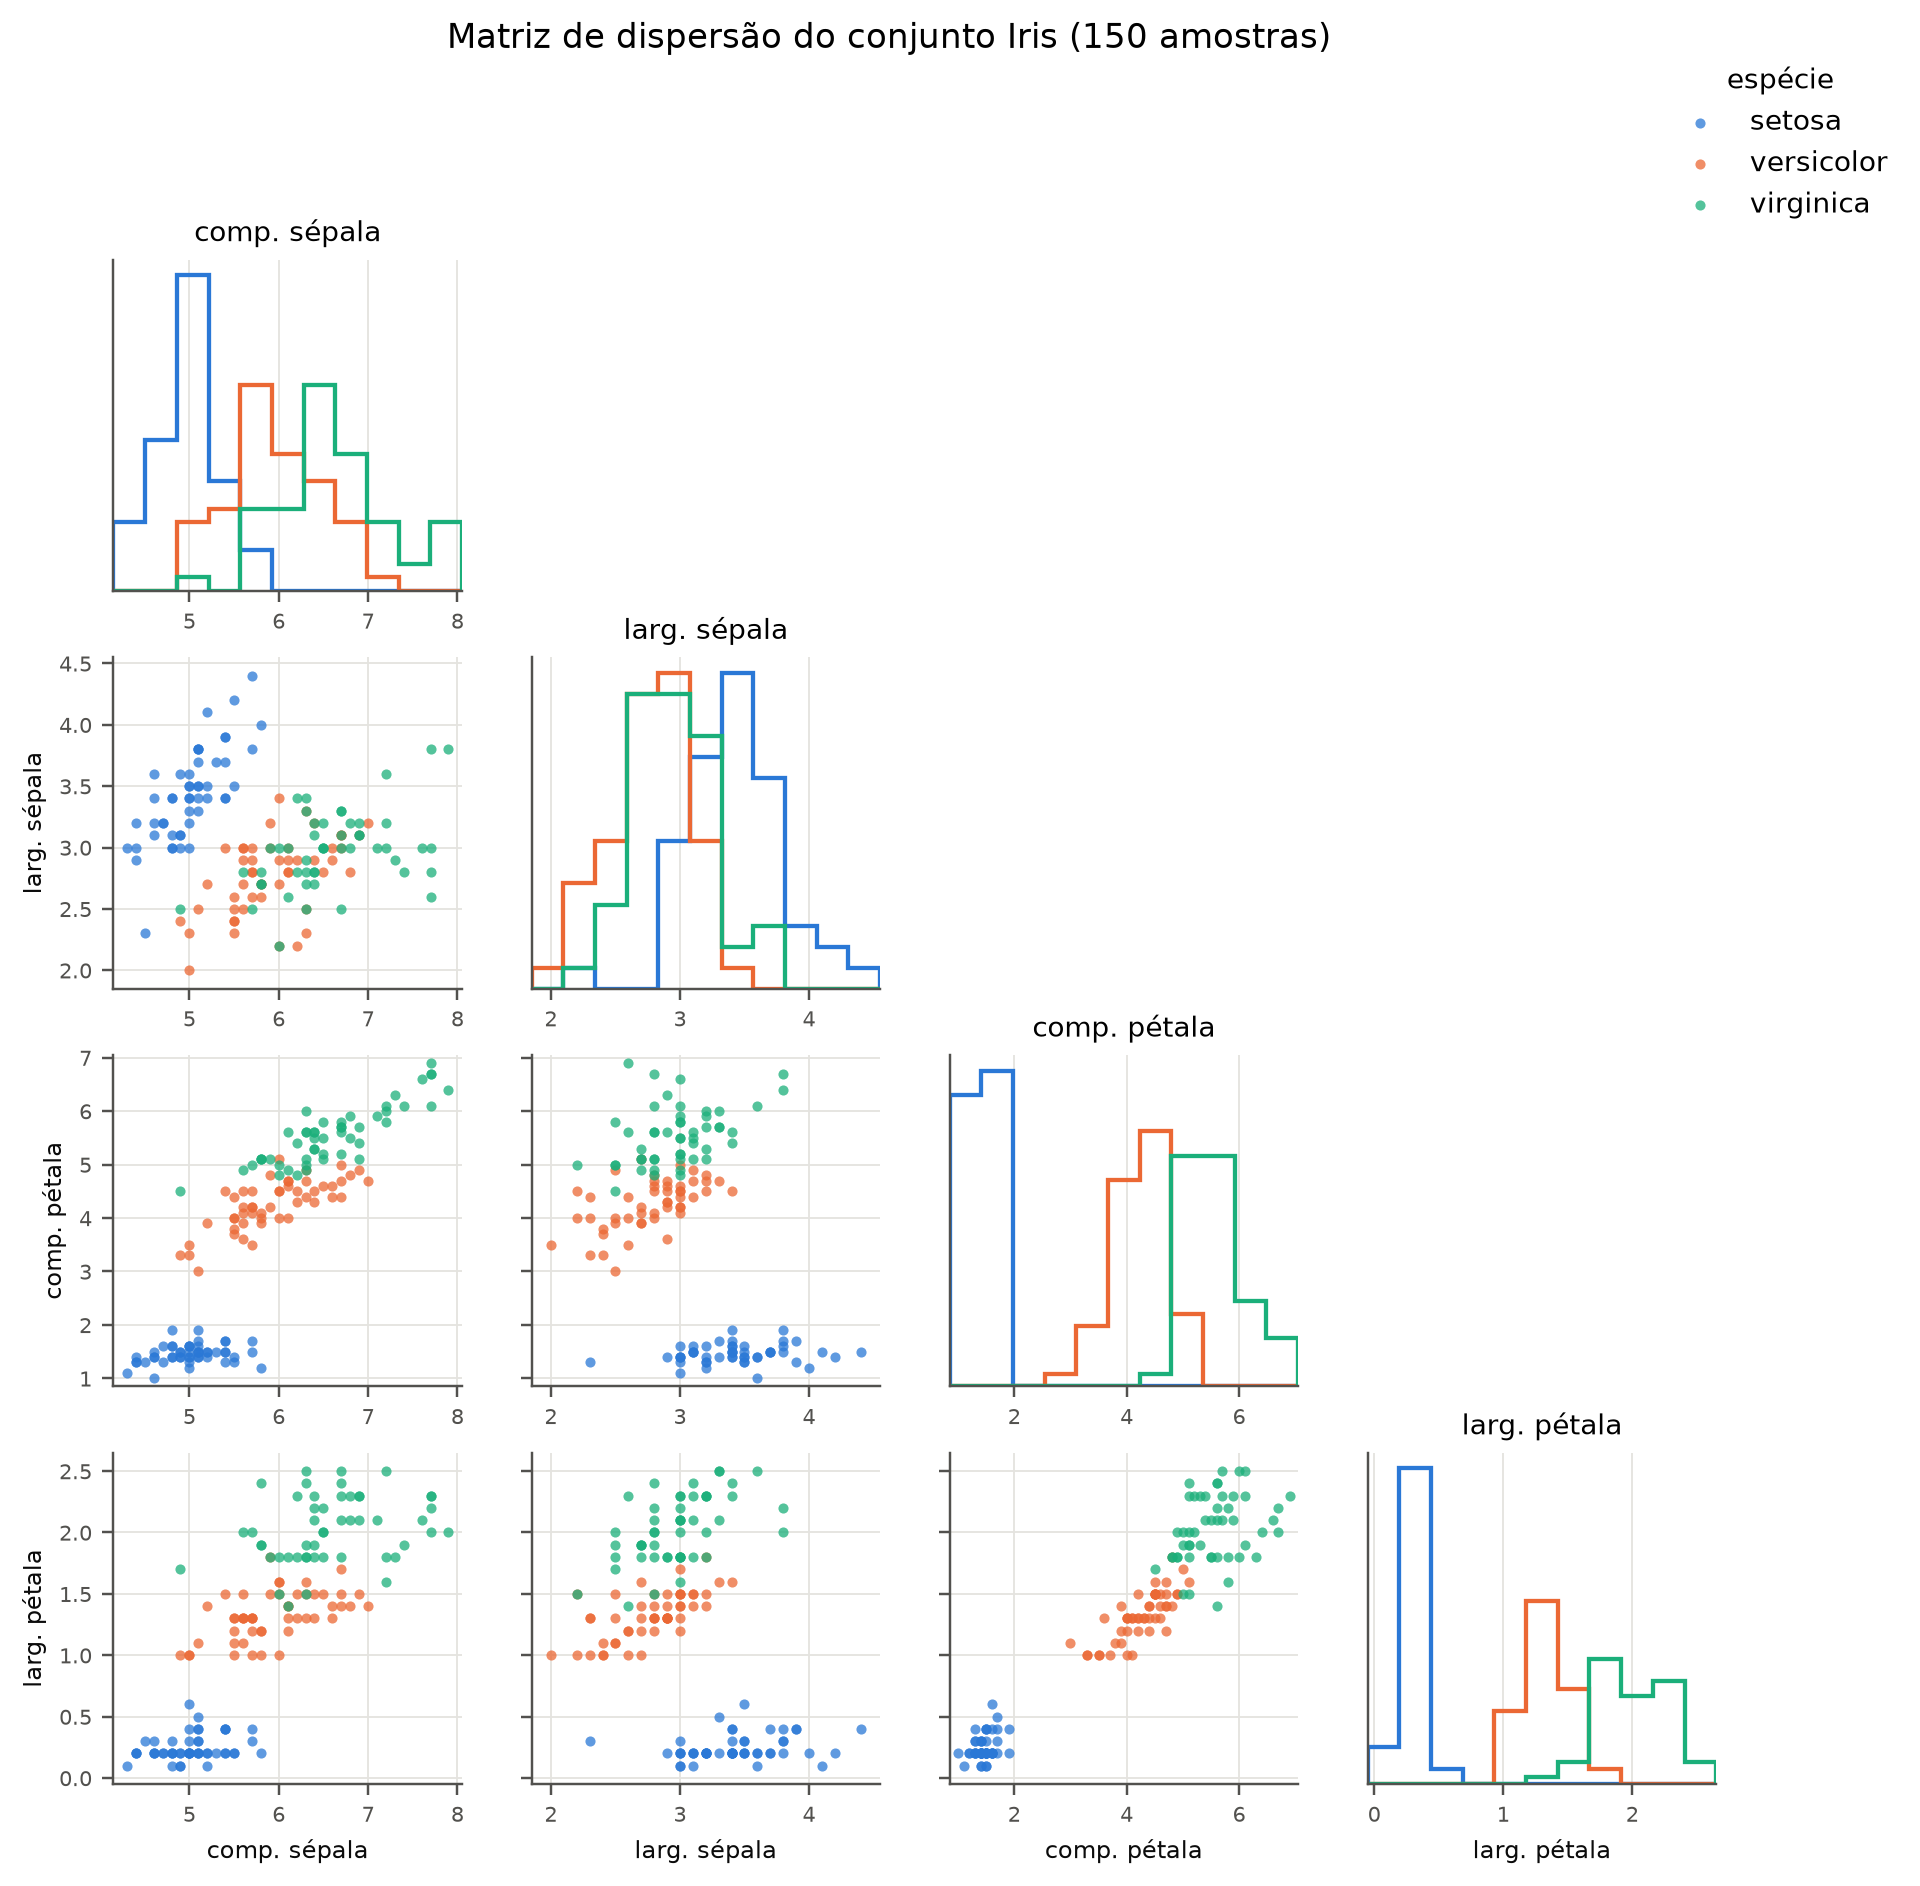
\includegraphics[width=0.72\textwidth]{fig_iris_dispersao.png}
	\caption{Matriz de dispersão dos quatro atributos. Abaixo da diagonal, dispersões dois a dois;
	na diagonal, histogramas por espécie. A \emph{setosa} (azul) forma um grupo isolado em todas as
	projeções que envolvem a pétala.}
	\label{fig:dispersao}
\end{figure}

\paragraph{A \emph{setosa} é separável.} Em qualquer gráfico que use comprimento ou largura da
pétala, os pontos azuis ocupam uma região própria, sem sobreposição com as demais espécies. Isso
significa que a classe é linearmente separável das outras duas: existe um hiperplano que a isola.

\paragraph{\emph{Versicolor} e \emph{virginica} se sobrepõem.} A fronteira entre as duas é difusa.
Há flores de \emph{versicolor} com pétalas tão grandes quanto as de \emph{virginica} e vice-versa.
Praticamente todo o erro de qualquer classificador razoável no Iris vem dessa região.

\paragraph{A sépala ajuda pouco.} A \figura{fig:boxplots} mostra que as distribuições de largura
da sépala das três espécies se sobrepõem quase completamente. O comprimento da sépala separa bem a
\emph{setosa}, mas confunde as outras duas. Em outras palavras: o problema tem duas variáveis
informativas e duas quase redundantes.

\begin{figure}[htbp]
	\centering
	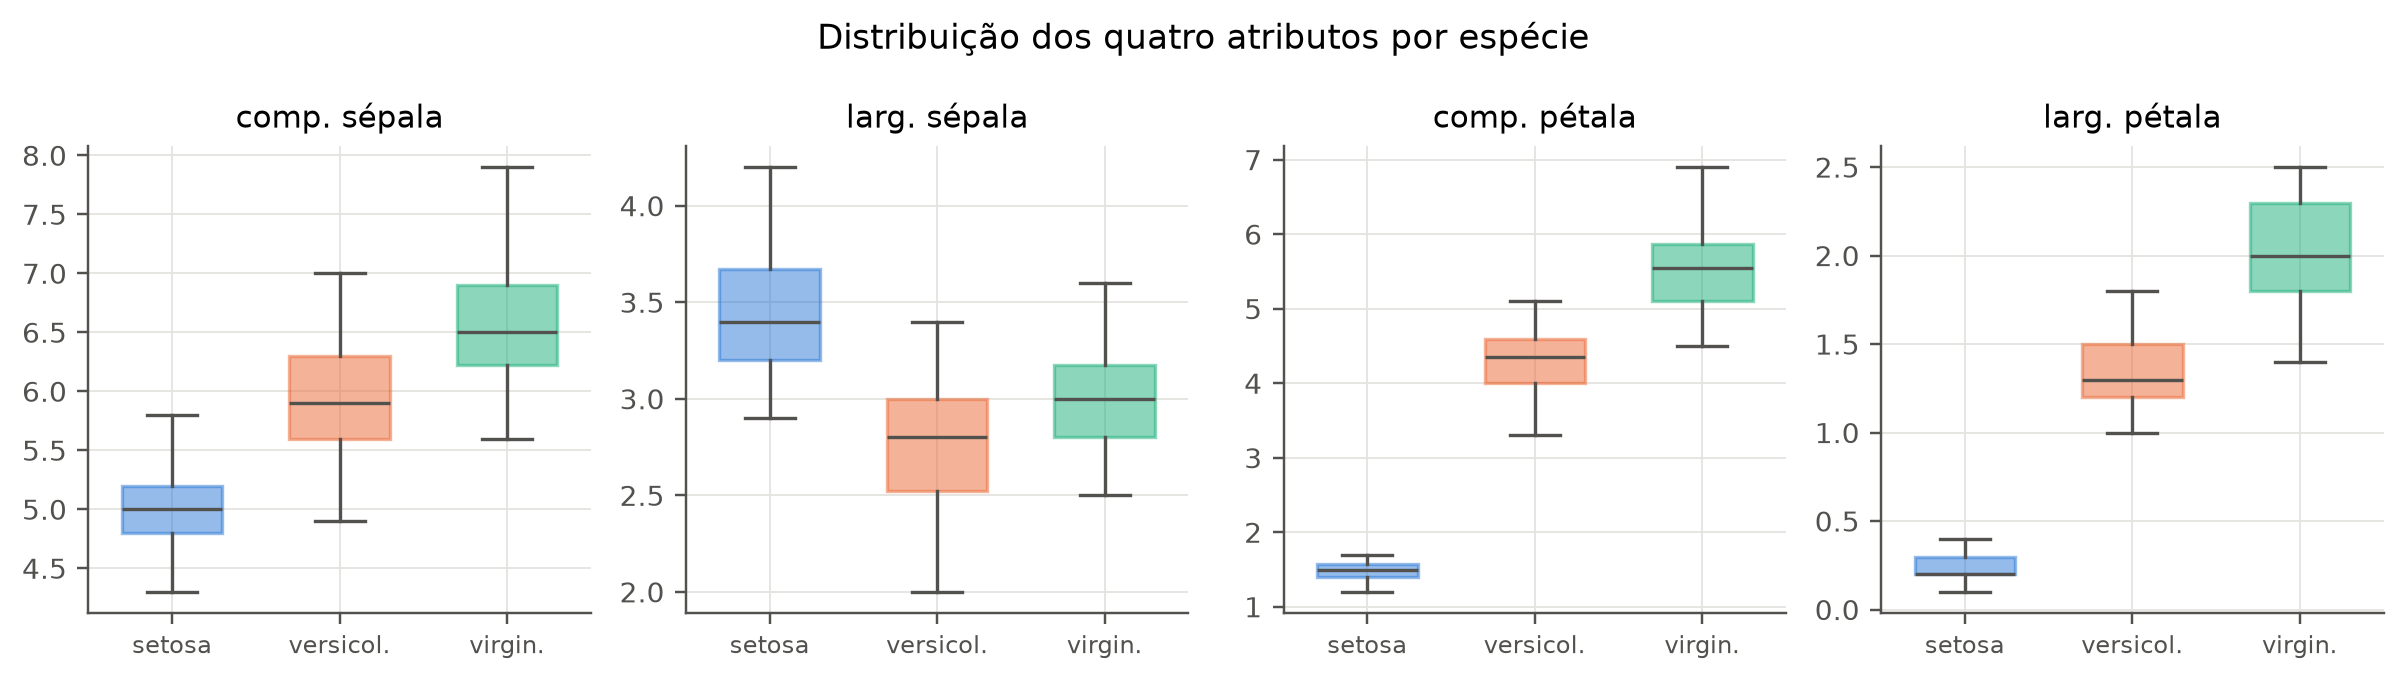
\includegraphics[width=\textwidth]{fig_iris_boxplots.png}
	\caption{Distribuições dos quatro atributos por espécie. As caixas vão do primeiro ao terceiro
	quartil, a linha central é a mediana e os bigodes se estendem até 1,5 vez o intervalo
	interquartil.}
	\label{fig:boxplots}
\end{figure}

A matriz de correlação (\figura{fig:correlacao}) confirma a leitura. Comprimento e largura da
pétala têm correlação de $0{,}96$; comprimento da sépala correlaciona $0{,}87$ com o comprimento da
pétala e $0{,}82$ com a largura da pétala. A largura da sépala é a variável mais independente:
$-0{,}43$ com o comprimento da pétala e $-0{,}37$ com a largura. Há, portanto, redundância
considerável: quatro medidas resumem essencialmente duas direções de variação.

\begin{figure}[htbp]
	\centering
	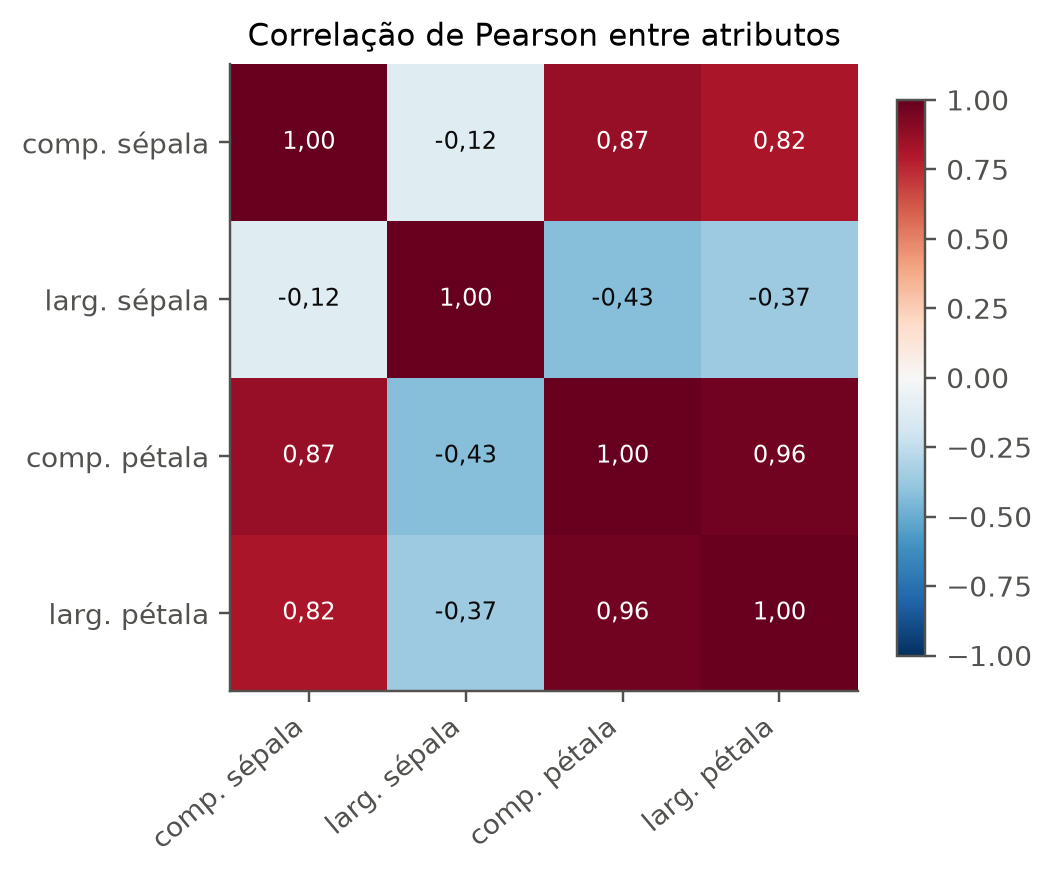
\includegraphics[width=0.62\textwidth]{fig_iris_correlacao.png}
	\caption{Correlação de Pearson entre os quatro atributos. Azul indica correlação positiva,
	vermelho, negativa.}
	\label{fig:correlacao}
\end{figure}

A análise de componentes principais torna essa redundância explícita. Depois de padronizar os
atributos, a primeira componente explica $73{,}0\,\%$ da variância e a segunda, $22{,}9\,\%$
(\figura{fig:pca}). Juntas, elas resumem $95{,}9\,\%$ da informação --- e, no plano formado por
elas, as três espécies aparecem em uma sequência ordenada, com a \emph{setosa} isolada à esquerda e
as outras duas ocupando uma faixa contínua à direita.

\begin{figure}[htbp]
	\centering
	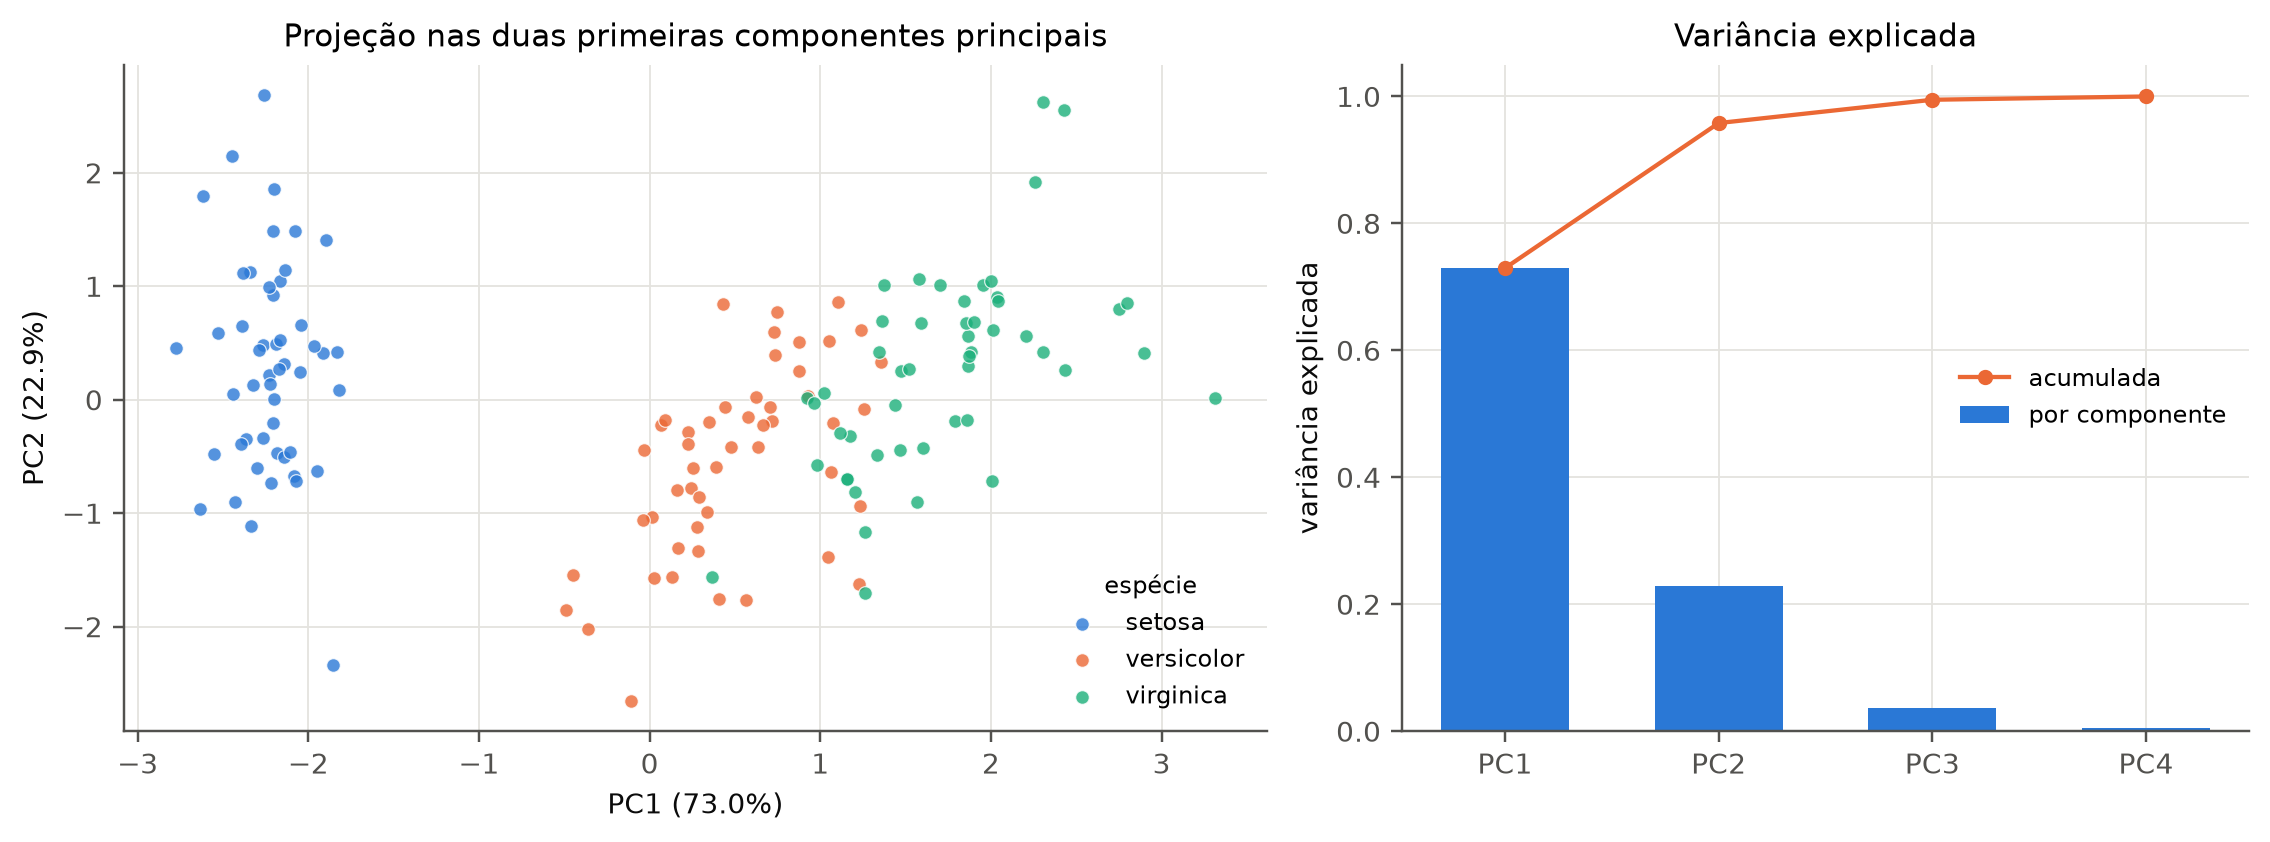
\includegraphics[width=\textwidth]{fig_iris_pca.png}
	\caption{Projeção nas duas primeiras componentes principais (atributos padronizados) e
	variância explicada por componente. A separação entre as espécies é quase inteiramente
	unidimensional.}
	\label{fig:pca}
\end{figure}

\subsection{O que esperar de um classificador}

A análise exploratória permite prever o desempenho antes de treinar qualquer modelo. Como a
\emph{setosa} é separável, espera-se acerto próximo de $100\,\%$ nessa classe. O erro deve se
concentrar na fronteira entre \emph{versicolor} e \emph{virginica}, onde alguns pontos são
ambiguos até para um especialista. Uma acurácia global entre $95\,\%$ e $98\,\%$ é o intervalo
plausível; muito acima disso sugere vazamento de informação ou sorte na divisão; muito abaixo
sugere erro de implementação.

Essa previsão é importante porque fornece um critério externo de sanidade. Quando um modelo
reporta $99{,}9\,\%$ em um conjunto com sobreposição visível, a primeira hipótese não é genialidade
do modelo, e sim algum problema no protocolo de avaliação --- por exemplo, padronizar os dados
antes de dividir treino e teste, ou ajustar hiperparâmetros no conjunto de teste.

\subsection{Limitações do conjunto}

O Iris é excelente para aprender, mas ruim para generalizar conclusões. Três limitações devem ser
registradas desde já.

\begin{itemize}
	\item \textbf{tamanho}: 150 amostras implicam intervalos de confiança largos. Um acerto a mais
	      ou a menos no conjunto de teste muda a acurácia em $2{,}2$ pontos percentuais;
	\item \textbf{dimensionalidade}: com quatro atributos e três classes, qualquer modelo tem
	      capacidade de sobra. O problema não testa a habilidade da rede de aprender representações
	      complexas;
	\item \textbf{quase separabilidade}: como as classes são quase linearmente separáveis, modelos
	      lineares competem de igual para igual com redes neurais, o que limita o que se pode
	      concluir sobre a vantagem de arquiteturas profundas.
\end{itemize}

Essas limitações não impedem o estudo da MLP; elas definem o que o estudo pode afirmar. O
\secao{sec:discussao} retoma o ponto com os resultados em mãos.

% =======================================================================================================
\section{Fundamentos da rede perceptron multicamadas}
\label{sec:mlp}

Esta seção constrói a MLP do zero. A ideia é que cada fórmula tenha uma interpretação e que o
leitor possa, ao final, implementar a rede em qualquer linguagem. A derivação completa da
retropropagação, com todas as passagens, está no Apêndice~\ref{ap:backprop}.

\subsection{Do neurônio artificial ao perceptron}

O modelo de McCulloch e Pitts \cite{mcculloch1943} descreve um neurônio como uma unidade que soma
entradas ponderadas e aplica um limiar. Em notação vetorial, com entradas
$\bx = (x_1,\dots,x_d)\T$, pesos $\bm{w} = (w_1,\dots,w_d)\T$ e viés $b$:

\begin{equation}
	z = \bm{w}\T \bx + b = \sum_{j=1}^{d} w_j x_j + b,
	\qquad
	a = f(z),
	\label{eq:neuronio}
\end{equation}

em que $f$ é a função de ativação. A \figura{fig:neuronio} representa essa unidade. O viés $b$
desempenha o papel de um peso associado a uma entrada constante igual a $1$; ele desloca a
fronteira de decisão e permite que ela não passe pela origem.

\begin{figure}[htbp]
	\centering
	\begin{tikzpicture}[>=Stealth,font=\small,node distance=8mm]
		\node (x1) at (0,1.9) {$x_1$};
		\node (x2) at (0,1.1) {$x_2$};
		\node (x3) at (0,0.3) {$\vdots$};
		\node (x4) at (0,-0.5) {$x_d$};
		\node[circle,draw,thick,minimum size=13mm,fill=blue!8] (soma) at (3.6,0.7) {$\Sigma$};
		\node[draw,thick,rounded corners=2pt,minimum width=13mm,minimum height=11mm,
		fill=orange!15] (ativ) at (5.6,0.7) {$f$};
		\node (saida) at (7.9,0.7) {$a = f(\bm{w}\T\bx+b)$};
		\node[circle,draw,minimum size=6mm,fill=gray!12] (bias) at (3.6,2.4) {$1$};
		\draw[->] (x1) -- node[above,font=\scriptsize,pos=0.45] {$w_1$} (soma);
		\draw[->] (x2) -- node[above,font=\scriptsize,pos=0.45] {$w_2$} (soma);
		\draw[->] (x3) -- node[above,font=\scriptsize,pos=0.5] {$\vdots$} (soma);
		\draw[->] (x4) -- node[below,font=\scriptsize,pos=0.45] {$w_d$} (soma);
		\draw[->] (bias) -- node[right,font=\scriptsize] {$b$} (soma);
		\draw[->,thick] (soma) -- node[above,font=\scriptsize] {$z$} (ativ);
		\draw[->,thick] (ativ) -- (saida);
		\node[font=\scriptsize,gray] at (0,-1.1) {entradas};
		\node[font=\scriptsize,gray] at (3.6,3.1) {viés};
	\end{tikzpicture}
	\caption{Unidade de um neurônio artificial: combinação linear das entradas seguida de uma
	ativação não linear. O viés $b$ é uma entrada constante que desloca o limiar de ativação.}
	\label{fig:neuronio}
\end{figure}

Um único neurônio com ativação degrau é o perceptron de Rosenblatt \cite{rosenblatt1958}. Sua
capacidade é limitada: ele só resolve problemas linearmente separáveis, e o contraexemplo clássico
é a função lógica XOR \cite{minsky1969}. A saída para essa limitação não é um neurônio mais
complexo, mas uma \emph{composição} de neurônios: a rede.

\subsection{Arquitetura e propagação direta}

Uma MLP organiza os neurônios em camadas. A camada $0$ é a entrada (os atributos), a camada $L$ é a
saída e as camadas $1,\dots,L-1$ são ocultas. Sejam $n_l$ o número de neurônios da camada $l$,
$\bW^{(l)} \in \R^{n_{l-1}\times n_l}$ a matriz de pesos que liga a camada $l-1$ à camada $l$ e
$\bb^{(l)} \in \R^{n_l}$ o vetor de vieses.

Com $m$ amostras organizadas em uma matriz $\bX \in \R^{m\times d}$ (uma amostra por linha), a
propagação direta é

\begin{align}
	\bA^{(0)} &= \bX, \label{eq:forward-a0}\\
	\bZ^{(l)} &= \bA^{(l-1)} \bW^{(l)} + \mathbf{1}_m \bb^{(l)\top},
	\qquad l = 1,\dots,L, \label{eq:forward-z}\\
	\bA^{(l)} &= f_l\!\left(\bZ^{(l)}\right),
	\qquad l = 1,\dots,L-1, \label{eq:forward-a}
\end{align}

em que $\mathbf{1}_m$ é o vetor de $m$ uns (o mesmo viés para todas as amostras) e $f_l$ é aplicada
elemento a elemento. Na saída, para classificação multiclasse, usa-se a função \emph{softmax}:

\begin{equation}
	p_{ik} = \frac{\exp\!\left(z_{ik}^{(L)}\right)}{\displaystyle\sum_{j=1}^{C}\exp\!\left(z_{ij}^{(L)}\right)},
	\qquad k = 1,\dots,C,
	\label{eq:softmax}
\end{equation}

com $C$ classes. A saída $\bp_i = (p_{i1},\dots,p_{iC})$ é uma distribuição de probabilidade sobre
as classes, e a previsão é $\hat{y}_i = \argmax_k p_{ik}$.

A \figura{fig:arquitetura} mostra a arquitetura usada como referência neste relatório, com quatro
entradas, duas camadas ocultas e três saídas. Cada ligação é um parâmetro a estimar.

\begin{figure}[htbp]
	\centering
	\begin{tikzpicture}[>=Stealth,font=\scriptsize,scale=0.95,transform shape]
		\def\dy{0.85}
		% entrada
		\foreach \i/\n in {1/x_1,2/x_2,3/x_3,4/x_4}{
			\node[circle,draw,thick,minimum size=0.62cm,fill=blue!10] (I\i) at (0,{(4.5-\i)*\dy}) {$\n$};
		}
		% oculta 1 (5 neurônios)
		\foreach \j in {1,...,5}{
			\node[circle,draw,thick,minimum size=0.62cm,fill=orange!15] (H1\j) at (2.9,{(5.5-\j)*\dy}) {};
		}
		% oculta 2 (4 neurônios)
		\foreach \k in {1,...,4}{
			\node[circle,draw,thick,minimum size=0.62cm,fill=orange!15] (H2\k) at (5.8,{(5-\k)*\dy}) {};
		}
		% saída
		\foreach \o/\n in {1/y_1,2/y_2,3/y_3}{
			\node[circle,draw,thick,minimum size=0.62cm,fill=green!12] (O\o) at (8.7,{(4-\o)*\dy}) {$\n$};
		}
		% vieses
		\node[circle,draw,minimum size=0.45cm,fill=gray!20] (B1) at (2.9,4.9) {$1$};
		\node[circle,draw,minimum size=0.45cm,fill=gray!20] (B2) at (5.8,4.4) {$1$};
		% conexões
		\foreach \i in {1,...,4} \foreach \j in {1,...,5} \draw[gray!55,line width=0.25pt] (I\i) -- (H1\j);
		\foreach \j in {1,...,5} \foreach \k in {1,...,4} \draw[gray!55,line width=0.25pt] (H1\j) -- (H2\k);
		\foreach \k in {1,...,4} \foreach \o in {1,...,3} \draw[gray!55,line width=0.25pt] (H2\k) -- (O\o);
		\foreach \j in {1,...,5} \draw[gray!80,dashed] (B1) -- (H1\j);
		\foreach \k in {1,...,4} \draw[gray!80,dashed] (B2) -- (H2\k);
		% rótulos
		\node[font=\scriptsize,above] at (0,3.1) {entrada};
		\node[font=\scriptsize,above] at (2.9,4.2) {oculta 1};
		\node[font=\scriptsize,above] at (5.8,3.65) {oculta 2};
		\node[font=\scriptsize,above] at (8.7,2.9) {saída};
		\node[font=\scriptsize,below] at (1.45,0.55) {$\bW^{(1)}$};
		\node[font=\scriptsize,below] at (4.35,0.55) {$\bW^{(2)}$};
		\node[font=\scriptsize,below] at (7.25,0.55) {$\bW^{(3)}$};
		\node[font=\scriptsize,above,gray] at (0,-0.55) {$d=4$};
		\node[font=\scriptsize,above,gray] at (2.9,-0.55) {$n_1=5$};
		\node[font=\scriptsize,above,gray] at (5.8,-0.9) {$n_2=4$};
		\node[font=\scriptsize,above,gray] at (8.7,-1.3) {$C=3$};
	\end{tikzpicture}
	\caption{Arquitetura de uma MLP com duas camadas ocultas. As linhas tracejadas representam os
	vieses, que funcionam como neurônios de entrada fixos em $1$.}
	\label{fig:arquitetura}
\end{figure}

\paragraph{Contagem de parâmetros.} Cada camada $l$ contribui com $n_{l-1}n_l$ pesos e $n_l$
vieses. Para a arquitetura $4$--$16$--$3$ adotada neste relatório:
\begin{equation}
	\underbrace{4 \times 16 + 16}_{\text{camada oculta}} \;+\;
	\underbrace{16 \times 3 + 3}_{\text{camada de saída}} = 64 + 16 + 48 + 3 = 131
	\label{eq:parametros}
\end{equation}
parâmetros, valor confirmado em execução (\parametrosMLP{}). A rede $4$--$5$--$4$--$3$ da
\figura{fig:arquitetura} teria $4\cdot5+5 + 5\cdot4+4 + 4\cdot3+3 = 20+5+20+4+12+3 = 64$
parâmetros. Comparar o número de parâmetros com o número de amostras é o primeiro teste de
viabilidade: com 150 amostras, uma rede com dezenas de milhares de parâmetros não tem como ser
estimada de forma confiável.

\subsection{Funções de ativação}

A não linearidade é o que distingue a MLP de uma regressão logística. Sem ela, a composição de
camadas colapsa em uma única transformação afim: $\bW^{(2)}f(\bW^{(1)}\bx) = \bW'\bx$ se $f$ é
linear. As funções mais usadas estão na \tabela{tab:ativacoes-math} e na
\figura{fig:ativacoes-curvas}.

\begin{table}[htbp]
	\centering
	\caption{Funções de ativação usuais, derivadas e faixa de saída.}
	\label{tab:ativacoes-math}
	\small
	\begin{tabular}{L{2.6cm} L{4.2cm} L{4.3cm} L{2.4cm}}
		\toprule
		\textbf{Nome} & \textbf{Função $f(z)$} & \textbf{Derivada $f'(z)$} & \textbf{Faixa} \\
		\midrule
		Identidade & $z$ & $1$ & $(-\infty,\infty)$ \\
		Logística (sigmoide) & $\dfrac{1}{1+e^{-z}}$ & $f(z)\left(1-f(z)\right)$ & $(0,1)$ \\
		Tangente hiperbólica & $\tanh(z) = \dfrac{e^{z}-e^{-z}}{e^{z}+e^{-z}}$ & $1-\tanh^2(z)$ & $(-1,1)$ \\
		ReLU & $\max(0,z)$ & $\indic[z>0]$ & $[0,\infty)$ \\
		Leaky ReLU & $\max(\alpha z, z)$ & $1$ se $z>0$; $\alpha$ caso contrário & $(-\infty,\infty)$ \\
		Softmax (saída) & $\dfrac{e^{z_k}}{\sum_j e^{z_j}}$ & ver \equacao{eq:softmax-jacobiano} & $(0,1)$ \\
		\bottomrule
	\end{tabular}
\end{table}

\begin{figure}[htbp]
	\centering
	\begin{tikzpicture}
		\begin{axis}[
			width=0.47\textwidth, height=5.2cm,
			xlabel={$z$}, ylabel={$f(z)$},
			domain=-4:4, samples=120, grid=both, grid style={gray!18},
			legend pos=north west, legend style={font=\scriptsize,draw=none,fill=white,fill opacity=0.8,text opacity=1},
			tick label style={font=\scriptsize}, label style={font=\small},
			title={Funções de ativação},
		]
			\addplot[blue,thick] {1/(1+exp(-x))}; \addlegendentry{logística}
			\addplot[orange,thick] {tanh(x)}; \addlegendentry{tanh}
			\addplot[green!55!black,thick] {max(0,x)}; \addlegendentry{ReLU}
			\addplot[gray,dashed,thick] {x}; \addlegendentry{identidade}
		\end{axis}
	\end{tikzpicture}\hfill
	\begin{tikzpicture}
		\begin{axis}[
			width=0.47\textwidth, height=5.2cm,
			xlabel={$z$}, ylabel={$f'(z)$},
			domain=-4:4, samples=200, grid=both, grid style={gray!18},
			legend pos=north east, legend style={font=\scriptsize,draw=none,fill=white,fill opacity=0.8,text opacity=1},
			tick label style={font=\scriptsize}, label style={font=\small},
			title={Derivadas},
			ymin=-0.1, ymax=1.15,
		]
			\addplot[blue,thick] {exp(-x)/(1+exp(-x))^2}; \addlegendentry{logística}
			\addplot[orange,thick] {1-tanh(x)^2}; \addlegendentry{tanh}
			\addplot[green!55!black,thick] {x>0 ? 1 : 0}; \addlegendentry{ReLU}
		\end{axis}
	\end{tikzpicture}
	\caption{Funções de ativação e suas derivadas. A derivada da logística e a da tangente
	hiperbólica se aproximam de zero nas caudas --- a origem do problema de gradiente que
	desaparece. A ReLU tem derivada constante igual a $1$ para $z>0$, o que preserva o sinal do
	gradiente em redes profundas.}
	\label{fig:ativacoes-curvas}
\end{figure}

\paragraph{Escolha da ativação.} A ReLU é o padrão em redes profundas por ser barata e por não
saturar no lado positivo \cite{he2015}. A \emph{tanh} é simétrica em relação à origem e costuma
convergir bem em redes pequenas com dados padronizados --- é a escolha do modelo deste relatório.
A logística é historicamente importante, mas satura nos dois lados e, por isso, treina mais
devagar. A identidade não é uma não linearidade: usá-la na camada oculta equivale a um modelo
linear, o que, no Iris, é quase tão bom quanto a rede (ver \secao{sec:resultados}).

\paragraph{Por que não usar degrau.} A função degrau tem derivada nula em quase toda parte e
indefinida em zero. Sem gradiente, não há retropropagação. Foi exatamente essa dificuldade que
manteve as redes neurais adormecidas entre as décadas de 1970 e 1980.

\subsection{Camada de saída e função de custo}
\label{sec:custo}

Para classificação multiclasse, a saída natural é a softmax \equacao{eq:softmax} combinada com a
entropia cruzada categórica. Com os rótulos codificados em \emph{one-hot}
$\by_i \in \{0,1\}^{C}$ ($y_{ik}=1$ se a amostra $i$ pertence à classe $k$), a perda média é

\begin{equation}
	\Loss(\bW,\bb) = -\frac{1}{m}\sum_{i=1}^{m}\sum_{k=1}^{C} y_{ik}\,\log p_{ik}
	\;+\; \frac{\lambda}{2}\sum_{l=1}^{L}\left\|\bW^{(l)}\right\|_F^2,
	\label{eq:cross-entropy}
\end{equation}

em que $\|\cdot\|_F$ é a norma de Frobenius e $\lambda \ge 0$ controla a regularização $L_2$.
No scikit-learn, o hiperparâmetro \texttt{alpha} corresponde a $\lambda$ (a penalidade é somada
como $\alpha\|\bW\|^2/2$). O primeiro termo é a entropia cruzada: ele é mínimo quando a
probabilidade atribuída à classe correta é $1$, e cresce sem limite quando ela se aproxima de $0$.

\paragraph{A derivada que faz tudo funcionar.} A combinação softmax com entropia cruzada tem uma
propriedade notável. Para uma amostra isolada,

\begin{equation}
	\frac{\partial \Loss}{\partial z_k^{(L)}} = p_k - y_k, \qquad k = 1,\dots,C.
	\label{eq:softmax-grad}
\end{equation}

Ou seja: o gradiente em relação aos \emph{scores} de saída é simplesmente o erro de probabilidade.
A demonstração está no Apêndice~\ref{ap:backprop}, mas a intuição é direta. A softmax tem
jacobiano
\begin{equation}
	\frac{\partial p_k}{\partial z_j} = p_k\left(\delta_{kj} - p_j\right),
	\label{eq:softmax-jacobiano}
\end{equation}
e a regra da cadeia aplicada a $-\sum_k y_k \log p_k$ produz vários termos que se cancelam, porque
$\sum_k y_k = 1$ e $\sum_k p_k = 1$. O resultado \equacao{eq:softmax-grad} é a razão pela qual
essa combinação é onipresente.

\paragraph{Por que não erro quadrático.} Poderia parecer natural minimizar
$\frac{1}{2}\sum_k (p_k-y_k)^2$. Com a softmax, o gradiente resultante seria proporcional a
$p_k(1-p_k)$ e, quando a rede erra com confiança ($p_k \approx 0$ para a classe correta), esse fator
leva o gradiente a zero: o modelo erra muito e aprende pouco. Com a entropia cruzada, o gradiente
$p_k - y_k$ é máximo justamente quando o erro é maior. Além disso, a entropia cruzada é convexa
em relação aos \emph{scores} de saída (embora não em relação aos pesos da rede).

\paragraph{Regularização $L_2$.} O termo $\frac{\lambda}{2}\|\bW\|_F^2$ pune pesos grandes,
suavizando a função aprendida. Sua contribuição ao gradiente é $\lambda\bW$, o que dá origem ao
nome \emph{weight decay}: a cada passo, os pesos são encolhidos na direção da origem antes de
receberem o empurrão do erro. No scikit-learn, \texttt{alpha} é o $\lambda$ dessa formulação.

\subsection{Retropropagação}
\label{sec:backprop}

O objetivo do treinamento é encontrar $\bW,\bb$ que minimizem \equacao{eq:cross-entropy}. Como a
perda depende dos pesos de forma composicional, o gradiente é obtido pela regra da cadeia,
aplicada da saída para a entrada --- daí o nome \emph{retropropagação}
\cite{rumelhart1986}.

Defina o \emph{erro} da camada $l$ como a derivada da perda em relação à pré-ativação:
\begin{equation}
	\bm{\Delta}^{(l)} = \frac{\partial \Loss}{\partial \bZ^{(l)}} \in \R^{m\times n_l}.
	\label{eq:delta}
\end{equation}
Na saída, por \equacao{eq:softmax-grad},
\begin{equation}
	\bm{\Delta}^{(L)} = \frac{1}{m}\left(\bP - \bY\right).
	\label{eq:delta-L}
\end{equation}
Para as camadas ocultas, aplica-se a regra da cadeia duas vezes (uma para atravessar a ativação,
outra para atravessar a matriz de pesos):
\begin{equation}
	\bm{\Delta}^{(l)} = \left(\bm{\Delta}^{(l+1)}\bW^{(l+1)\top}\right) \odot f_l'\!\left(\bZ^{(l)}\right),
	\qquad l = L-1,\dots,1,
	\label{eq:delta-rec}
\end{equation}
em que $\odot$ é o produto de Hadamard (elemento a elemento). Com os erros de cada camada, os
gradientes dos parâmetros são

\begin{align}
	\frac{\partial \Loss}{\partial \bW^{(l)}} &= \bA^{(l-1)\top}\bm{\Delta}^{(l)} + \lambda\bW^{(l)},
	\label{eq:grad-W}\\
	\frac{\partial \Loss}{\partial \bb^{(l)}} &= \sum_{i=1}^{m}\bm{\Delta}^{(l)}_{i,:}
	= \mathbf{1}_m^{\top} \bm{\Delta}^{(l)}.
	\label{eq:grad-b}
\end{align}

A \figura{fig:fluxo-gradiente} resume o ciclo: a informação sobe pela rede (propagação direta), a
perda é calculada, e o erro desce pela rede (retropropagação) carregando, em cada camada, a
informação de quanto cada peso contribuiu para o erro final.

\begin{figure}[htbp]
	\centering
	\begin{tikzpicture}[>=Stealth,font=\small,node distance=10mm,
		caixa/.style={draw,thick,rounded corners=3pt,minimum height=9mm,align=center,fill=blue!6},
		seta/.style={->,thick}]
		\node[caixa] (x) {entrada\\$\bX$};
		\node[caixa,right=of x] (f) {propagação\\direta};
		\node[caixa,right=of f] (l) {perda\\$\Loss$};
		\node[caixa,below=of l] (g) {gradiente\\$\partial\Loss/\partial\bm{\theta}$};
		\node[caixa,left=of g] (b) {retro-\\propagação};
		\node[caixa,left=of b] (u) {atualização\\$\bm{\theta}\leftarrow\bm{\theta}-\eta\,\bm{g}$};
		\draw[seta] (x) -- (f);
		\draw[seta] (f) -- (l);
		\draw[seta] (l) -- (g);
		\draw[seta] (g) -- (b);
		\draw[seta] (b) -- (u);
		\draw[seta] (u) |- (f);
		\node[font=\scriptsize,gray,above] at (2.35,0.55) {pesos $\bm{\theta}$};
	\end{tikzpicture}
	\caption{Ciclo de treinamento. A propagação direta e a retropropagação têm o mesmo custo
	assintótico: $O\!\left(m\sum_l n_{l-1}n_l\right)$, isto é, proporcional ao número de
	parâmetros.}
	\label{fig:fluxo-gradiente}
\end{figure}

\paragraph{Custo computacional.} Uma passagem direta custa $O(m\sum_l n_{l-1}n_l)$ operações. A
retropropagação custa o mesmo, com uma constante pequena. Isso é decisivo: calcular o gradiente
por diferenças finitas custaria $O(P)$ passagens diretas, com $P$ o número de parâmetros, o que
seria inviável para redes reais. A retropropagação é o que torna o treinamento possível.

\paragraph{Verificação numérica.} Como a retropropagação é fácil de implementar errado, todo
código sério é validado por diferenças centrais:
\begin{equation}
	\frac{\partial \Loss}{\partial \theta_i} \approx
	\frac{\Loss(\theta_i+\varepsilon) - \Loss(\theta_i-\varepsilon)}{2\varepsilon},
	\qquad \varepsilon \approx 10^{-6},
	\label{eq:gradcheck}
\end{equation}
e compara-se com o gradiente analítico pelo erro relativo
$\left|g_{\text{ana}} - g_{\text{num}}\right| / \left(\left|g_{\text{ana}}\right| + \left|g_{\text{num}}\right|\right)$.
Valores abaixo de $10^{-4}$ indicam implementação correta. A
\figura{fig:gradiente} mostra o resultado obtido: erro máximo de \erroGrad{}, o que confirma a
derivação e o código.

\subsection{Otimização}
\label{sec:otimizacao}

Com o gradiente em mãos, o treinamento é um problema de otimização iterativa. A atualização mais
simples é o gradiente descendente:
\begin{equation}
	\bm{\theta}_{t+1} = \bm{\theta}_t - \eta\,\nabla_{\bm{\theta}}\Loss(\bm{\theta}_t),
	\label{eq:gd}
\end{equation}
com taxa de aprendizado $\eta > 0$. Calcular o gradiente com todas as $m$ amostras a cada passo é
caro e redundante; o \emph{gradiente descendente estocástico} (SGD) usa uma amostra ou um
\emph{minilote} $\mathcal{B}$ de tamanho $B$:
\begin{equation}
	\bm{\theta}_{t+1} = \bm{\theta}_t - \eta\,\widehat{\nabla}\Loss(\bm{\theta}_t),
	\qquad
	\widehat{\nabla}\Loss = \frac{1}{B}\sum_{i\in\mathcal{B}}\nabla \ell_i.
	\label{eq:sgd}
\end{equation}
O estimador é não viesado, mas ruidoso. Esse ruído, que à primeira vista parece um defeito, ajuda
a escapar de pontos de sela e de mínimos ruins.

\paragraph{Momento.} Para suavizar a trajetória, acumula-se uma velocidade:
\begin{align}
	\bm{v}_{t} &= \mu\,\bm{v}_{t-1} - \eta\,\bm{g}_t, \label{eq:momentum}\\
	\bm{\theta}_{t} &= \bm{\theta}_{t-1} + \bm{v}_{t}, \label{eq:momentum-upd}
\end{align}
com $\mu \in [0,1)$ (tipicamente $0{,}9$). A variante de Nesterov avalia o gradiente na posição
``adiantada'' $\bm{\theta} + \mu\bm{v}$, o que antecipa a correção.

\paragraph{Adam.} O otimizador Adam \cite{kingma2015} mantém médias móveis do gradiente e do
gradiente ao quadrado, com correção de viés:
\begin{align}
	\bm{m}_t &= \beta_1\bm{m}_{t-1} + (1-\beta_1)\bm{g}_t, \label{eq:adam-m}\\
	\bm{v}_t &= \beta_2\bm{v}_{t-1} + (1-\beta_2)\bm{g}_t^{\,2}, \label{eq:adam-v}\\
	\widehat{\bm{m}}_t &= \frac{\bm{m}_t}{1-\beta_1^{t}}, \qquad
	\widehat{\bm{v}}_t = \frac{\bm{v}_t}{1-\beta_2^{t}}, \label{eq:adam-bias}\\
	\bm{\theta}_t &= \bm{\theta}_{t-1} - \eta\,
	\frac{\widehat{\bm{m}}_t}{\sqrt{\widehat{\bm{v}}_t}+\epsilon},
	\label{eq:adam-upd}
\end{align}
com $\beta_1 = 0{,}9$, $\beta_2 = 0{,}999$ e $\epsilon = 10^{-8}$ como padrões. A divisão por
$\sqrt{\widehat{\bm{v}}}$ normaliza o passo por parâmetro: coordenadas com gradiente
sistematicamente grande recebem passos menores. É por isso que o Adam é bastante insensível à
escala dos atributos --- propriedade explorada no \secao{sec:resultados}.

\paragraph{Taxa de aprendizado.} É o hiperparâmetro mais importante. Taxa pequena faz o
treinamento lento e pode parar em região ruim; taxa grande faz a perda oscilar ou divergir. No
scikit-learn, o padrão de \texttt{MLPClassifier} é $\eta = 10^{-3}$ com Adam, e a taxa é reduzida
por $\eta_t = \eta_0 / t^{\,p}$ quando \texttt{learning\_rate='invscaling'}.

\subsection{Regularização e controle de capacidade}
\label{sec:regularizacao}

Um modelo com parâmetros demais ajusta o ruído do treino e generaliza mal. As técnicas de
regularização limitam essa capacidade de formas complementares.

\begin{itemize}
	\item \textbf{$L_2$ (weight decay)}: penaliza a norma dos pesos
	      \equacao{eq:cross-entropy}, mantendo-os pequenos e a função mais suave;
	\item \textbf{parada antecipada} (\emph{early stopping}): acompanha a perda em um conjunto de
	      validação e interrompe o treino quando ela para de melhorar, devolvendo os melhores pesos
	      \cite{prechelt1998}. No scikit-learn, isso é controlado por \texttt{early\_stopping},
	      \texttt{validation\_fraction} e \texttt{n\_iter\_no\_change};
	\item \textbf{\emph{dropout}}: durante o treino, desliga neurônios ao acaso com probabilidade
	      $q$, forçando representações redundantes \cite{srivastava2014}. Não é usado aqui, porque
	      com 150 amostras o efeito é mais ruído do que regularização;
	\item \textbf{aumento de dados}: não se aplica diretamente a medidas de flores, mas é a
	      regularização mais eficaz em imagens e áudio;
	\item \textbf{redução da arquitetura}: menos neurônios, menos parâmetros, menos variância.
\end{itemize}

\subsection{Inicialização}

Se todos os pesos começam iguais, todos os neurônios de uma camada recebem o mesmo gradiente e
permanecem idênticos --- a chamada quebra de simetria nunca ocorre. Por isso a inicialização é
aleatória, mas com variância calibrada para preservar a escala dos sinais entre camadas.

A inicialização de Xavier/Glorot \cite{glorot2010} escolhe
\begin{equation}
	\Var\!\left(W_{ij}^{(l)}\right) = \frac{2}{n_{l-1}+n_l},
	\label{eq:xavier}
\end{equation}
adequada para ativações simétricas como a \emph{tanh}. Para a ReLU, a inicialização de He
\cite{he2015} usa
\begin{equation}
	\Var\!\left(W_{ij}^{(l)}\right) = \frac{2}{n_{l-1}},
	\label{eq:he}
\end{equation}
porque a ReLU descarta metade dos sinais. O scikit-learn usa uma inicialização uniforme do tipo
Xavier para todas as ativações, o que é adequado para redes pequenas como as deste estudo.

\subsection{Capacidade, aproximação universal e generalização}
\label{sec:universal}

O teorema da aproximação universal \cite{cybenko1989,hornik1989} garante que, para qualquer função
contínua $g$ em um compacto e qualquer $\epsilon>0$, existe uma rede com uma camada oculta
suficientemente larga tal que $|F(\bx)-g(\bx)|<\epsilon$ para todo $\bx$ no domínio. Isso é uma
garantia de \emph{existência}, não de aprendizado: ela não diz quantos neurônios são necessários,
nem que o gradiente descendente encontrará os pesos certos, nem que a rede generalizará para
dados não vistos.

A distinção entre \emph{capacidade} e \emph{generalização} é central. A capacidade mede o que a
rede \emph{pode} representar; a generalização mede o que ela \emph{aprende} com os dados
disponíveis. Um modelo com capacidade muito acima do necessário tem variância alta: pequenas
mudanças no treino mudam muito a função aprendida. O equilíbrio é o compromisso
viés--variância, e a validação cruzada é a ferramenta prática para encontrá-lo.

\subsection{Pré-processamento}
\label{sec:preproc}

\paragraph{Padronização.} Redes neurais são sensíveis à escala dos atributos. O procedimento
usual é o \emph{z-score}:
\begin{equation}
	z_{ij} = \frac{x_{ij} - \hat{\mu}_j}{\hat{\sigma}_j},
	\label{eq:zscore}
\end{equation}
com $\hat{\mu}_j$ e $\hat{\sigma}_j$ estimados \textbf{apenas no conjunto de treino} e depois
aplicados ao teste. Estimar a média e o desvio no conjunto completo antes de dividir é uma forma
clássica de vazamento de informação \cite{kaufman2012}: o teste passa a influenciar o
pré-processamento, e a estimativa de desempenho fica otimista.

No Iris, como os quatro atributos já estão em centímetros e em faixas próximas, a padronização
tem efeito pequeno; ela é mantida por boa prática e porque, em problemas com escalas
heterogêneas, é indispensável.

\paragraph{Codificação da saída.} Para $C$ classes, os rótulos são convertidos em vetores
\emph{one-hot} de dimensão $C$. Internamente, o scikit-learn faz essa conversão e usa softmax na
saída quando há mais de duas classes; com duas classes, usa um único neurônio com ativação
logística.

\subsection{O algoritmo completo}

O \figura{fig:pseudocodigo} reúne as peças em pseudocódigo. É útil compará-lo com a implementação
em NumPy do \secao{sec:impl}, que segue exatamente estes passos.

\begin{figure}[htbp]
	\centering
	\fbox{\begin{minipage}{0.92\textwidth}
		\small
		\textbf{Algoritmo 1 --- Treinamento de uma MLP por retropropagação}
		\begin{enumerate}[label=\arabic*.,leftmargin=6mm]
			\item padronizar as entradas usando estatísticas do treino;
			\item inicializar $\bW^{(l)}$ e $\bb^{(l)}$ para $l=1,\dots,L$;
			\item \textbf{para} cada época \textbf{faça}
			\begin{enumerate}[label=\arabic*.\arabic*,leftmargin=8mm]
				\item embaralhar as amostras e dividir em minilotes;
				\item \textbf{para} cada minilote $\mathcal{B}$ \textbf{faça}
				\begin{enumerate}[label=(\alph*),leftmargin=8mm]
					\item propagação direta: $\bZ^{(l)}=\bA^{(l-1)}\bW^{(l)}+\bb^{(l)}$,
					      $\bA^{(l)}=f_l(\bZ^{(l)})$ até $\bP=\softmax(\bZ^{(L)})$;
					\item perda: $\Loss$ por \equacao{eq:cross-entropy};
					\item erro de saída: $\bm{\Delta}^{(L)}=(\bP-\bY)/|\mathcal{B}|$;
					\item \textbf{para} $l=L-1$ até $1$: $\bm{\Delta}^{(l)}=
					      (\bm{\Delta}^{(l+1)}\bW^{(l+1)\top})\odot f_l'(\bZ^{(l)})$;
					\item gradientes por \equacao{eq:grad-W} e \equacao{eq:grad-b};
					\item atualizar $\bm{\theta}$ com Adam, \equacao{eq:adam-upd};
				\end{enumerate}
				\item avaliar a perda de validação; se não melhorar por $p$ épocas, parar;
			\end{enumerate}
			\item devolver os pesos da época com melhor validação.
		\end{enumerate}
	\end{minipage}}
	\caption{Pseudocódigo do treinamento. A ordem dos laços (época, minilote, camada) determina o
	custo: cada época custa uma passagem direta e uma reversa por amostra.}
	\label{fig:pseudocodigo}
\end{figure}

% =======================================================================================================
\section{Metodologia experimental}
\label{sec:metodo}

Um resultado sem protocolo não é um resultado: é uma coincidência documentada. Esta seção descreve
como o modelo foi avaliado, por que cada escolha foi feita e quais são suas limitações. O objetivo
é que qualquer leitor possa repetir a análise e obter os mesmos números.

\subsection{Visão geral}

O protocolo tem cinco etapas:

\begin{enumerate}
	\item \textbf{separação}: divisão estratificada em treino (70\,\%) e teste (30\,\%), com o teste
	      reservado e usado uma única vez;
	\item \textbf{seleção}: comparação de arquiteturas, ativações e regularização por validação
	      cruzada \emph{apenas no treino};
	\item \textbf{treinamento final}: ajuste do modelo escolhido em todo o conjunto de treino;
	\item \textbf{avaliação}: uma única medida no conjunto de teste, com intervalo de confiança;
	\item \textbf{comparação}: repetição do procedimento para modelos alternativos, com as mesmas
	      dobras, e teste estatístico pareado.
\end{enumerate}

A separação entre \emph{seleção} e \emph{avaliação final} é o ponto mais importante. Se o mesmo
conjunto serve para escolher hiperparâmetros e para reportar desempenho, o resultado fica otimista:
o modelo foi escolhido, entre muitas opções, justamente por ter ido bem naquele conjunto. A
validação cruzada dentro do treino resolve a seleção; o teste, intocado, fornece a estimativa
honesta.

\subsection{Divisão treino/teste}

A divisão usa amostragem \emph{estratificada}: a proporção de cada classe é preservada nos dois
subconjuntos. Com 150 amostras e 30\,\% para teste, cada classe contribui com 15 amostras no teste
e 35 no treino, totalizando \nTeste{} e \nTreino{} amostras, respectivamente. A semente é fixa
(\texttt{random\_state=42}), de modo que a divisão é sempre a mesma.

\begin{figure}[htbp]
	\centering
	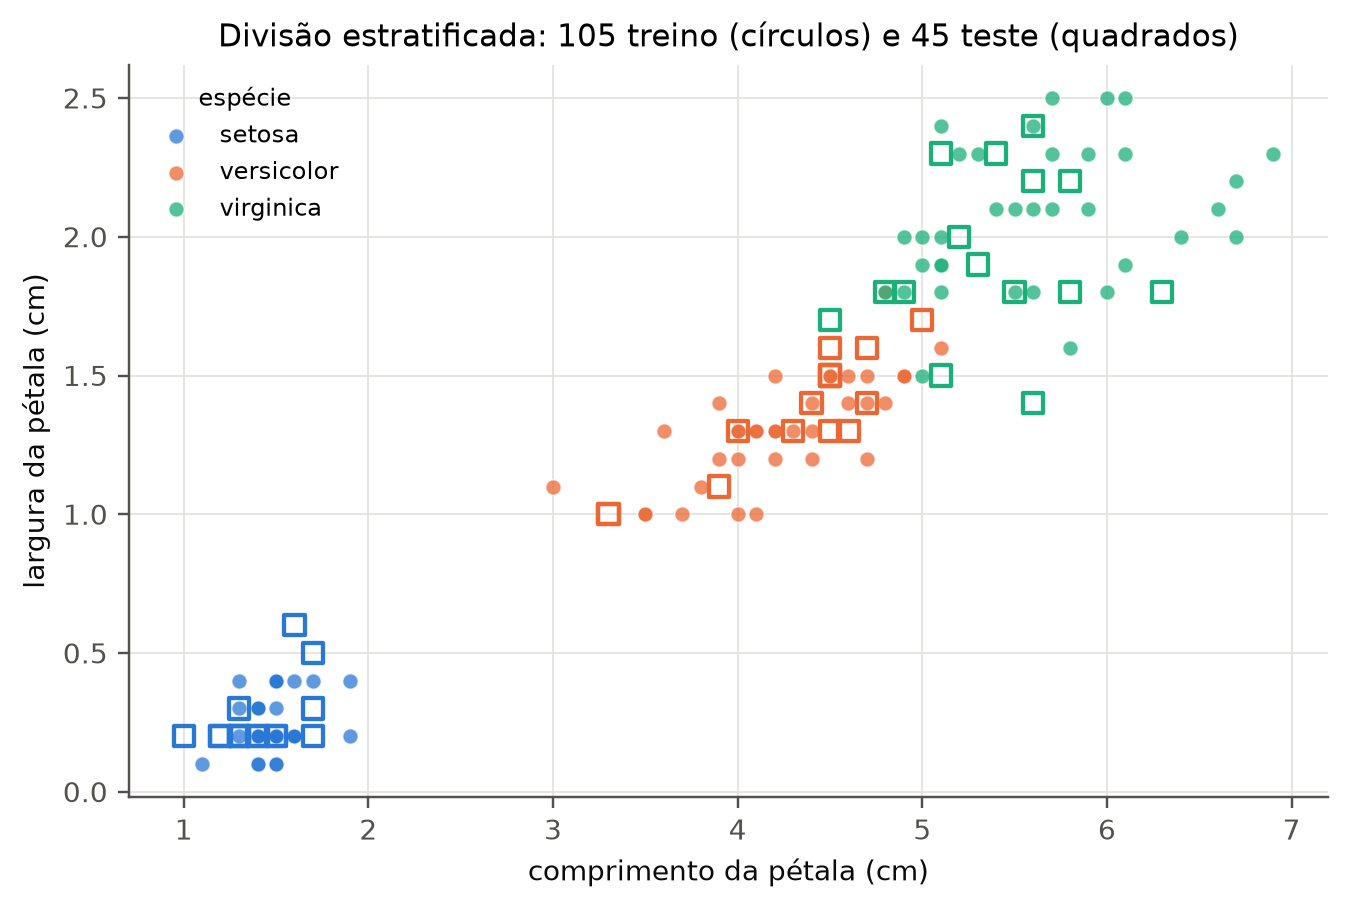
\includegraphics[width=0.72\textwidth]{fig_divisao_treino_teste.png}
	\caption{Divisão estratificada no plano das duas variáveis mais informativas. Círculos são
	amostras de treino (\nTreino{}) e quadrados vazados são amostras de teste (\nTeste{}). A
	proporção de cada espécie é preservada nos dois subconjuntos.}
	\label{fig:divisao}
\end{figure}

\paragraph{Por que estratificar.} Com 150 amostras, uma divisão puramente aleatória pode deixar
uma classe sub-representada no teste, o que aumenta a variância da estimativa. A estratificação
garante que o teste reflita a composição do problema.

\paragraph{Por que não usar o teste para nada além da medida final.} Cada vez que se olha o teste
e se toma uma decisão com base nele, ele deixa de ser um teste. Ajustar hiperparâmetros,
escolher a semente ou descartar um resultado ``estranho'' com base no teste contamina a
estimativa \cite{kaufman2012}.

\subsection{Validação cruzada}

A validação cruzada $k$-fold divide o conjunto de treino em $k$ partes iguais e, em cada rodada,
usa uma parte para validação e as outras $k-1$ para ajuste. Ao final, cada amostra foi usada
exatamente uma vez para validação. O estimador é a média das $k$ medidas:

\begin{equation}
	\widehat{\text{acc}}_{\text{CV}} = \frac{1}{k}\sum_{j=1}^{k} \text{acc}_j,
	\qquad
	\widehat{\text{se}} = \frac{s}{\sqrt{k}},
	\quad s^2 = \frac{1}{k-1}\sum_{j=1}^{k}\left(\text{acc}_j - \widehat{\text{acc}}_{\text{CV}}\right)^2.
	\label{eq:cv}
\end{equation}

Neste trabalho usa-se $k=5$ com estratificação, repetido $R=5$ vezes com sementes diferentes,
totalizando 25 medidas. A repetição reduz a dependência de uma partição específica
\cite{kohavi1995}. O desvio-padrão reportado é o das 25 dobras, não o erro-padrão da média: ele
mede a variabilidade entre partições, que é o que interessa para comparar configurações.

A \figura{fig:kfold} ilustra o esquema com $k=5$: em cada linha, o bloco destacado é a dobra de
validação e os demais são de treino.

\begin{figure}[htbp]
	\centering
	\begin{tikzpicture}[font=\scriptsize,x=0.9cm,y=0.9cm]
		\foreach \r in {1,...,5}{
			\foreach \c in {1,...,5}{
				\pgfmathtruncatemacro{\teste}{\r==\c}
				\ifnum\teste=1
					\fill[red!35] (\c-1,-\r) rectangle ++(1,0.8);
				\else
					\fill[blue!12] (\c-1,-\r) rectangle ++(1,0.8);
				\fi
				\draw[gray!70] (\c-1,-\r) rectangle ++(1,0.8);
			}
			\node[left] at (0,-\r+0.4) {rodada \r};
		}
		\foreach \c in {1,...,5}{
			\node[below] at (\c-0.5,-5.05) {dobra \c};
		}
		\node[anchor=west,fill=red!35,draw=gray!70,minimum width=0.5cm,minimum height=0.3cm] at (5.4,-1.2) {};
		\node[anchor=west] at (6.0,-1.2) {validação};
		\node[anchor=west,fill=blue!12,draw=gray!70,minimum width=0.5cm,minimum height=0.3cm] at (5.4,-2.2) {};
		\node[anchor=west] at (6.0,-2.2) {treino};
	\end{tikzpicture}
	\caption{Esquema da validação cruzada $k$-fold com $k=5$. Cada amostra é usada uma vez para
	validação e quatro vezes para treino. A estimativa final é a média das cinco rodadas.}
	\label{fig:kfold}
\end{figure}

\paragraph{Vazamento de informação.} O pré-processamento faz parte do modelo e deve ser ajustado
dentro de cada dobra. Por isso o código usa um \texttt{Pipeline}: a padronização é ajustada apenas
nas amostras de treino da dobra e aplicada às de validação. Se a padronização fosse ajustada no
conjunto completo, a média e o desvio conteriam informação do conjunto de validação --- vazamento
sutil, mas real \cite{kaufman2012}.

\subsection{Seleção de hiperparâmetros}

As varreduras usam 3 repetições de 5 dobras (15 ajustes por configuração), o que mantém o custo
baixo e já é suficiente para revelar tendências. O modelo final é escolhido pelos resultados
dessas varreduras e reavaliado no teste:

\begin{itemize}
	\item \textbf{arquitetura}: nove configurações, de $(4)$ a $(128,64)$, e a contagem de
	      parâmetros correspondente;
	\item \textbf{ativação}: ReLU, \emph{tanh}, logística e identidade, com a mesma arquitetura
	      $(16,8)$;
	\item \textbf{regularização}: $\alpha \in \{10^{-6},\dots,10^{2}\}$, em escala logarítmica, com
	      a arquitetura $(32,16)$;
	\item \textbf{taxa de aprendizado}: SGD com momento, taxas de $10^{-3}$ a $5\times10^{-1}$.
\end{itemize}

A configuração adotada --- uma camada oculta com 16 neurônios, ativação \emph{tanh} e
$\alpha = 10^{-2}$ --- é uma escolha de compromisso entre as três varreduras: a \emph{tanh} foi a
ativação com melhor acurácia, $\alpha = 10^{-2}$ está no centro da faixa estável e 16 neurônios é
uma capacidade intermediária, nem mínima nem excessiva. Ela não é o máximo absoluto de nenhuma
varredura isolada --- a rede de 4 neurônios teve acurácia ligeiramente maior ---, e essa diferença
está dentro do ruído entre dobras. Como a escolha foi feita sobre os dados de treino, a estimativa
de validação cruzada do modelo final é ligeiramente otimista; o conjunto de teste, mantido à
parte, é a medida que não sofre esse efeito.

\subsection{Métricas de avaliação}
\label{sec:metricas}

Para um problema de classificação, a acurácia isolada esconde informação. As métricas usadas são
definidas a seguir, para uma classe $k$ com verdadeiros positivos $TP_k$, falsos positivos $FP_k$
e falsos negativos $FN_k$.

\begin{align}
	\text{acurácia} &= \frac{1}{n}\sum_{i=1}^{n}\indic\left[\hat{y}_i = y_i\right],
	\label{eq:acc}\\
	\text{precisão}_k &= \frac{TP_k}{TP_k+FP_k}, \qquad
	\text{revocação}_k = \frac{TP_k}{TP_k+FN_k},
	\label{eq:pr}\\
	F_{1,k} &= \frac{2\,\text{precisão}_k\,\text{revocação}_k}{\text{precisão}_k+\text{revocação}_k},
	\label{eq:f1}\\
	F_1^{\text{macro}} &= \frac{1}{C}\sum_{k=1}^{C} F_{1,k}. \label{eq:f1macro}
\end{align}

A precisão responde ``quando o modelo diz classe $k$, ele acerta?''. A revocação responde ``de
tudo que era classe $k$, quanto o modelo encontrou?''. O $F_1$ é a média harmônica das duas e pune
desequilíbrios. A média \emph{macro} dá o mesmo peso a todas as classes, independentemente do
tamanho; é a escolha correta quando as classes importam igualmente --- como aqui.

\paragraph{Entropia cruzada.} Para avaliar a \emph{calibração} das probabilidades, usa-se
\begin{equation}
	\text{LogLoss} = -\frac{1}{n}\sum_{i=1}^{n}\sum_{k=1}^{C} y_{ik}\log p_{ik},
	\label{eq:logloss}
\end{equation}
que penaliza confiança indevida. Um modelo pode ter acurácia alta e LogLoss ruim se acertar com
probabilidade $0{,}51$ em vez de $0{,}95$. Neste relatório, a LogLoss aparece nas varreduras
porque ela distingue configurações que a acurácia considera empatadas.

\paragraph{Matriz de confusão.} A matriz $C_{jk}$ conta quantas amostras da classe $j$ foram
previstas como $k$. Ela mostra \emph{para onde} vão os erros, o que a acurácia não mostra. No
\secao{sec:resultados}, a matriz revela que os erros se concentram na fronteira
\emph{versicolor}--\emph{virginica}.

\subsection{Incerteza das estimativas}

Com $n=45$ amostras de teste, uma acurácia de $93{,}3\,\%$ corresponde a 42 acertos. O intervalo de
confiança de Wilson, adequado para proporções com $n$ pequeno, é
\begin{equation}
	\frac{\hat{p} + \frac{z^2}{2n} \pm z\sqrt{\frac{\hat{p}(1-\hat{p})}{n} + \frac{z^2}{4n^2}}}{1+\frac{z^2}{n}},
	\qquad z = 1{,}96,
	\label{eq:wilson}
\end{equation}
com $\hat{p}$ a proporção observada. Para 42 acertos em 45, o intervalo vai de \icLo{} a \icHi{} ---
uma amplitude de quase 16 pontos percentuais. Essa largura não é um defeito do método: é a
informação disponível em 45 amostras. Reportar apenas o valor pontual seria esconder metade do
resultado.

\subsection{Comparação estatística entre modelos}

Comparar médias de validação cruzada sem teste estatístico é frágil, porque as dobras são
correlacionadas e as diferenças são pequenas. Como todos os modelos são avaliados nas
\emph{mesmas} 25 dobras, os resultados formam amostras pareadas. Aplica-se o teste de Wilcoxon
para amostras pareadas \cite{dietterich1998}, que não pressupõe normalidade:

\begin{enumerate}
	\item calculam-se as diferenças $d_i = \text{acc}_i^{A} - \text{acc}_i^{B}$ para as 25 dobras;
	\item descartam-se as diferenças nulas e ordenam-se os valores absolutos restantes;
	\item a estatística $W$ é a soma dos postos das diferenças positivas;
	\item compara-se $W$ com a distribuição nula para obter o valor $p$.
\end{enumerate}

Um valor $p < 0{,}05$ indica que a diferença é difícil de explicar por azar na partição das
dobras. Como são feitas três comparações, uma correção para múltiplos testes seria conservadora;
os valores são reportados sem correção, mas interpretados com cautela.

\subsection{Reprodutibilidade}

Todos os experimentos usam a semente $42$ para a divisão treino/teste, para a inicialização dos
pesos e para as partições da validação cruzada. As versões são Python 3.15, NumPy 2.5,
scikit-learn 1.9 e Matplotlib 3.11. A execução completa produz as figuras, as tabelas e o arquivo
de números citados no texto; se qualquer número mudar, o texto é recompilado com o valor novo.
Essa amarração entre código e documento é a forma mais simples de evitar a deriva entre o que foi
feito e o que foi escrito.

% =======================================================================================================
\section{Implementação}
\label{sec:impl}

O relatório usa duas implementações independentes da mesma rede: a do scikit-learn, madura e
otimizada, e uma implementação manual em NumPy, escrita para tornar a matemática visível. A
concordância entre as duas é, ela mesma, uma forma de validação.

\subsection{Organização do código}

O script \texttt{mlp\_iris.py} é organizado em etapas numeradas, na ordem em que aparecem no
relatório:

\begin{enumerate}
	\item leitura dos dados e análise exploratória;
	\item estudo de arquiteturas;
	\item estudo de funções de ativação;
	\item estudo da regularização $L_2$;
	\item estudo da taxa de aprendizado;
	\item curvas de treinamento e de aprendizado;
	\item divisão treino/teste e métricas finais;
	\item fronteiras de decisão e importância de atributos;
	\item visualização dos pesos;
	\item verificação numérica do gradiente e implementação em NumPy;
	\item comparação com modelos de referência e testes estatísticos.
\end{enumerate}

Cada etapa grava seus resultados em arquivo: métricas em CSV, figuras em PNG e tabelas em LaTeX.
Isso permite que o documento incorpore as tabelas diretamente, sem transcrição manual.

\subsection{O pipeline do scikit-learn}

O modelo é definido como um \texttt{Pipeline} de dois passos: padronização e MLP. A vantagem não é
estética: dentro da validação cruzada, o \texttt{Pipeline} garante que o \texttt{StandardScaler}
seja ajustado apenas na dobra de treino, eliminando o vazamento discutido no
\secao{sec:metodo}.

\begin{lstlisting}[caption={Definição do modelo principal (extrato de \texttt{mlp\_iris.py}).},label={lst:pipeline}]
def mlp(hidden=(16, 8), ativacao="relu", alpha=1e-3, semente=42,
        solver="adam", lr=1e-3, max_iter=3000, early_stopping=False):
    """Pipeline padronizacao + MLP (ajustado dentro de cada dobra)."""
    return make_pipeline(
        StandardScaler(),
        MLPClassifier(hidden_layer_sizes=hidden, activation=ativacao, alpha=alpha,
                      solver=solver, learning_rate_init=lr, max_iter=max_iter,
                      early_stopping=early_stopping, validation_fraction=0.15,
                      n_iter_no_change=40, random_state=semente),
    )

MLP_PRINCIPAL = dict(hidden=(16,), ativacao="tanh", alpha=1e-2)
\end{lstlisting}

Os hiperparâmetros têm o seguinte significado:

\begin{itemize}
	\item \texttt{hidden\_layer\_sizes}: tupla com o número de neurônios de cada camada oculta;
	\item \texttt{activation}: função de ativação das camadas ocultas;
	\item \texttt{alpha}: coeficiente $\lambda$ da penalidade $L_2$;
	\item \texttt{solver}: \texttt{adam}, \texttt{sgd} ou \texttt{lbfgs};
	\item \texttt{learning\_rate\_init}: taxa de aprendizado inicial $\eta_0$;
	\item \texttt{max\_iter}: número máximo de épocas;
	\item \texttt{early\_stopping}: ativa a parada antecipada com \texttt{validation\_fraction}
	      dos dados de treino;
	\item \texttt{n\_iter\_no\_change}: paciência, em épocas, antes de parar.
\end{itemize}

\subsection{Implementação manual em NumPy}

A implementação manual segue exatamente as equações do \secao{sec:mlp}. A classe
\texttt{MLPNumPy} guarda $\bW^{(1)},\bb^{(1)},\bW^{(2)},\bb^{(2)}$ e implementa a propagação
direta, a perda com regularização, a retropropagação e o passo de Adam.

\begin{lstlisting}[caption={Núcleo da implementação manual: propagação direta e retropropagação.},label={lst:numpy}]
def forward(self, X):
    z1 = X @ self.W1 + self.b1        # (m, h)  pre-ativacao da oculta
    a1 = self._f(z1)                  # (m, h)  ativacao da oculta
    z2 = a1 @ self.W2 + self.b2       # (m, C)  escores da saida
    return z1, a1, z2, _softmax(z2)   # (m, C)  probabilidades

def perda(self, X, y):
    _, _, _, p = self.forward(X)
    Y = _onehot(y)
    ce = -np.mean(np.sum(Y * np.log(p + 1e-12), axis=1))
    reg = 0.5 * self.alpha * (np.sum(self.W1 ** 2) + np.sum(self.W2 ** 2))
    return ce + reg

def backward(self, X, y):
    m = len(y)
    z1, a1, _, p = self.forward(X)
    Y = _onehot(y)
    d2 = (p - Y) / m                        # Delta^(2) = (P - Y)/m
    gW2 = a1.T @ d2 + self.alpha * self.W2  # gradiente + L2
    gb2 = d2.sum(0)
    d1 = (d2 @ self.W2.T) * self._df(z1)    # Delta^(1)
    gW1 = X.T @ d1 + self.alpha * self.W1
    gb1 = d1.sum(0)
    return {"W1": gW1, "b1": gb1, "W2": gW2, "b2": gb2}
\end{lstlisting}

O laço de treinamento aplica Adam, com as equações \equacao{eq:adam-m}--\equacao{eq:adam-upd},
a minilotes de 16 amostras embaralhadas a cada época:

\begin{lstlisting}[caption={Laço de treinamento com Adam (extrato).},label={lst:adam}]
for ep in range(epocas):
    ordem = rng.permutation(len(y))
    for i in range(0, len(y), lote):
        idx = ordem[i:i + lote]
        g = self.backward(X[idx], y[idx])
        t += 1
        for k in params:
            m[k] = b1 * m[k] + (1 - b1) * g[k]
            v[k] = b2 * v[k] + (1 - b2) * g[k] ** 2
            mh = m[k] / (1 - b1 ** t)       # correcao de vies
            vh = v[k] / (1 - b2 ** t)
            params[k] -= lr * mh / (np.sqrt(vh) + eps)
\end{lstlisting}

A \figura{fig:implementacao} compara as duas implementações. Com a mesma arquitetura
(8 neurônios ocultos), a implementação manual e a do scikit-learn alcançam exatamente a mesma
acurácia no teste (\accNumpy{} e \accSklearn{}), e a curva de perda da versão manual decresce de
forma suave, com as oscilações típicas do treinamento por minilotes.

\begin{figure}[htbp]
	\centering
	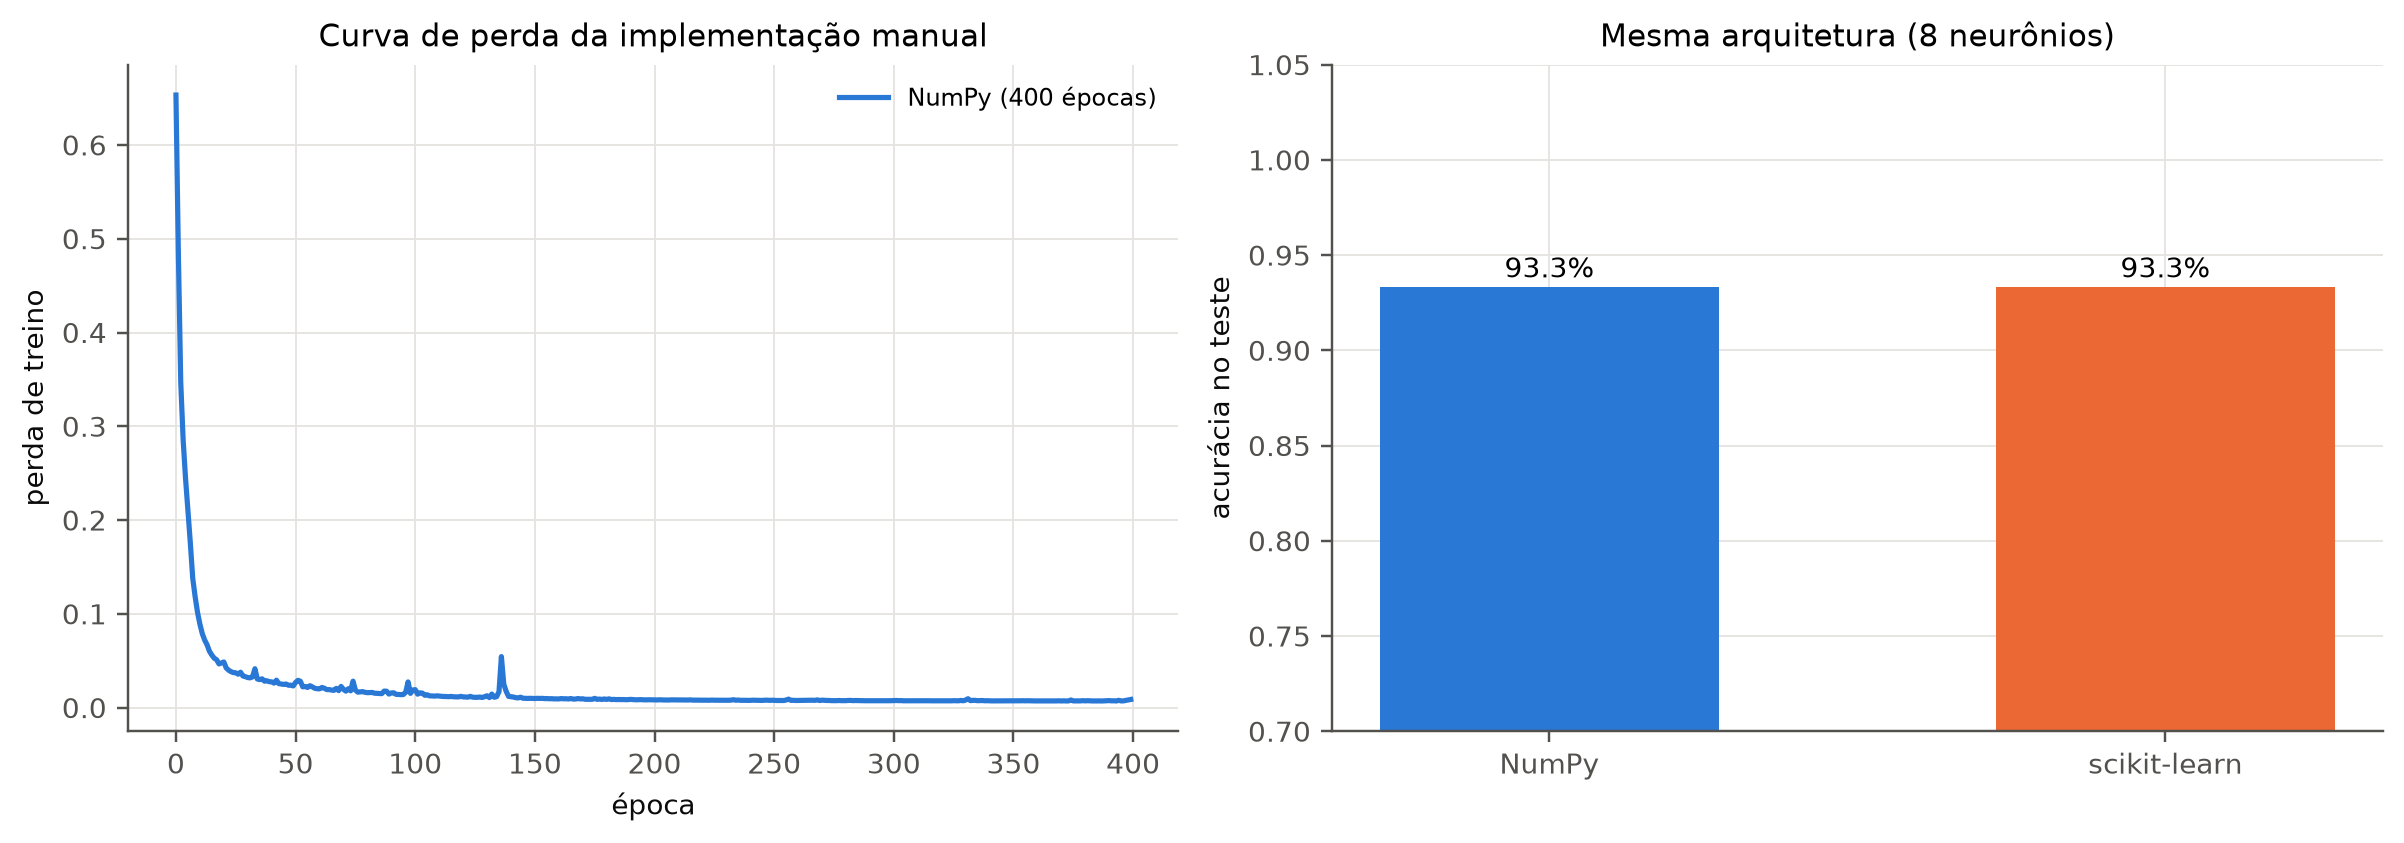
\includegraphics[width=\textwidth]{fig_implementacao.png}
	\caption{À esquerda, curva de perda da implementação manual em NumPy (400 épocas, Adam,
	minilotes de 16). À direita, acurácia no conjunto de teste das duas implementações com a mesma
	arquitetura.}
	\label{fig:implementacao}
\end{figure}

\subsection{Verificação numérica do gradiente}

A retropropagação é a parte mais sujeita a erro de implementação, porque envolve transposições e
produtos elemento a elemento que ``quase'' funcionam quando estão errados. O teste padrão compara
o gradiente analítico com uma aproximação por diferenças centrais, \equacao{eq:gradcheck}, em uma
rede pequena ($4$--$5$--$3$, ativação \emph{tanh}) e em um subconjunto de amostras.

O resultado está na \figura{fig:gradiente}. Os pontos caem praticamente sobre a diagonal
identidade, e o erro relativo máximo é \erroGrad{} --- ordens de grandeza abaixo do limiar de
$10^{-4}$ usado na prática. Isso confirma tanto a derivação quanto o código: se houvesse um erro
de sinal, de transposição ou de normalização, o erro relativo seria da ordem de $10^{-1}$ ou
maior.

\begin{figure}[htbp]
	\centering
	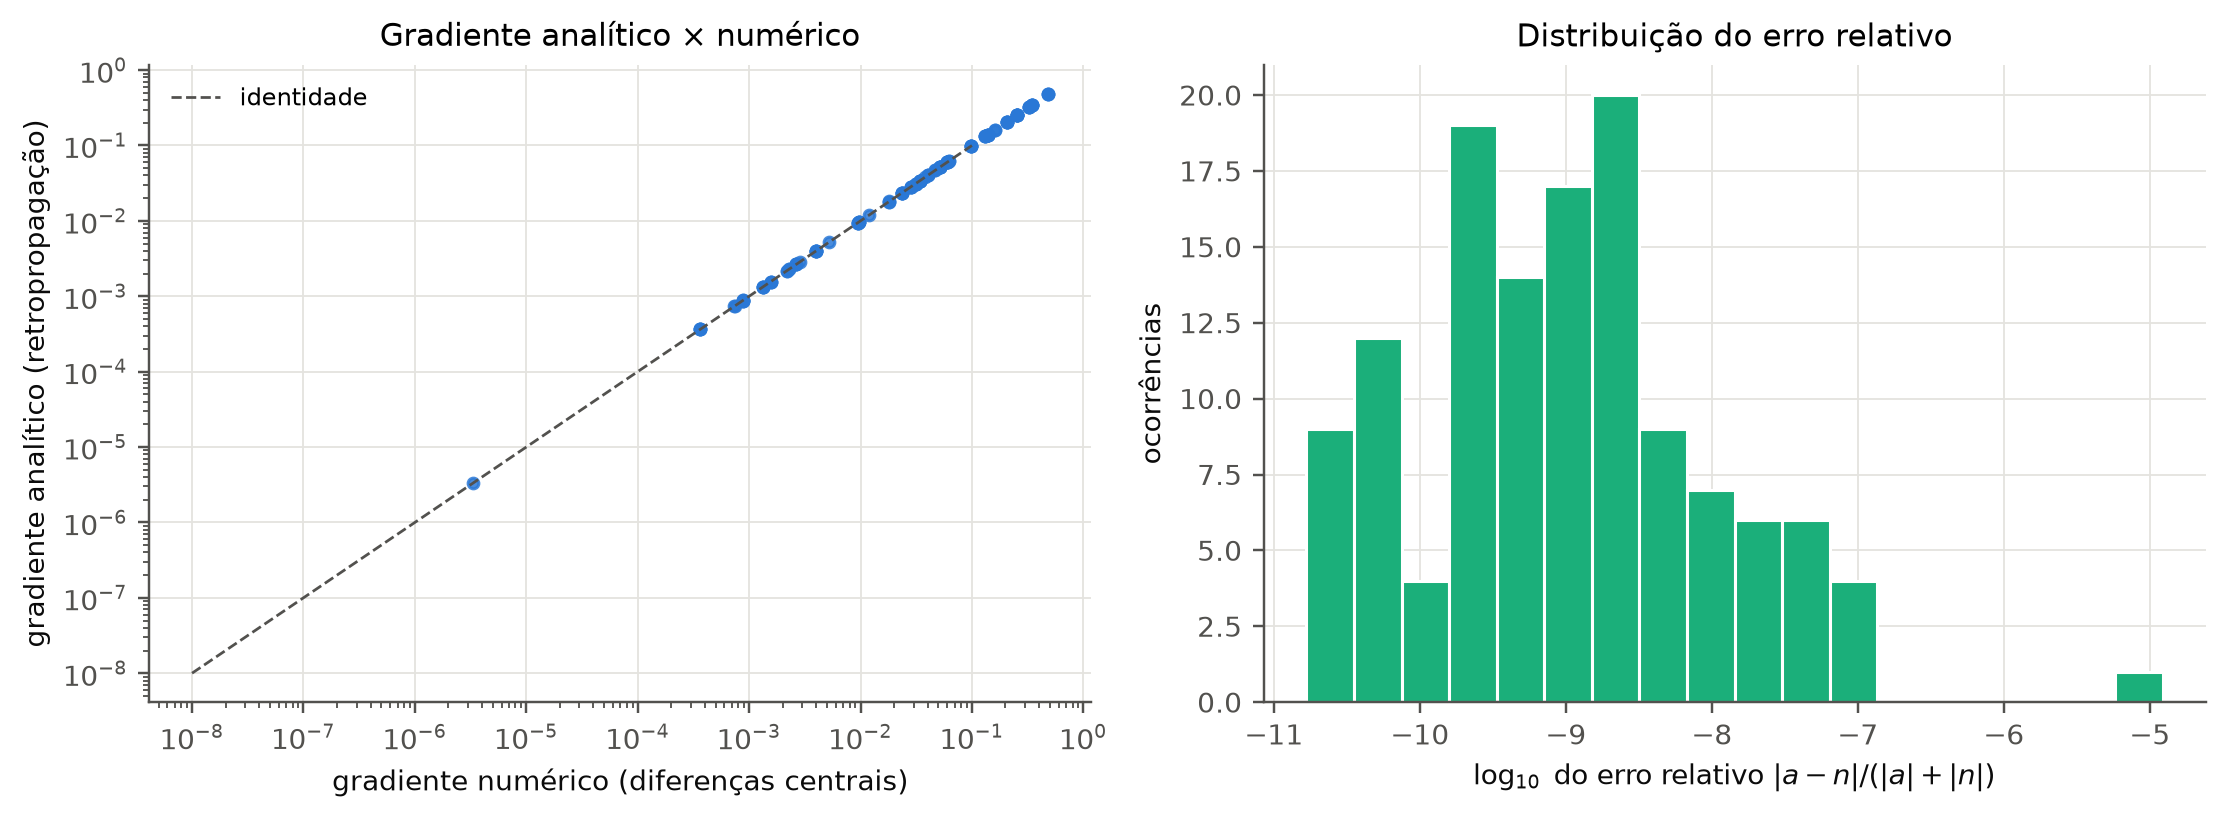
\includegraphics[width=\textwidth]{fig_gradiente.png}
	\caption{Verificação do gradiente. À esquerda, gradiente analítico contra numérico para os
	parâmetros amostrados; a linha tracejada é a identidade. À direita, distribuição do erro
	relativo, em escala logarítmica.}
	\label{fig:gradiente}
\end{figure}

\begin{table}[htbp]
	\centering
	\caption{Erro relativo da checagem de gradiente por matriz de parâmetros.}
	\label{tab:gradiente}
	% gerado automaticamente por mlp_iris.py - nao editar

\begin{tabular}{lrrr}
\toprule
\textbf{parâmetro} & \textbf{amostras} & \textbf{erro máximo} & \textbf{erro médio} \\
\midrule
W1 & 60 & $6{,}8\times10^{-8}$ & $1{,}2\times10^{-8}$ \\
b1 & 5 & $1{,}2\times10^{-5}$ & $2{,}5\times10^{-6}$ \\
W2 & 60 & $4{,}2\times10^{-9}$ & $1{,}3\times10^{-9}$ \\
b2 & 3 & $7{,}4\times10^{-9}$ & $3{,}2\times10^{-9}$ \\
\bottomrule
\end{tabular}

\end{table}

\subsection{Detalhes de engenharia}

Três decisões de implementação merecem registro, porque afetam a reprodutibilidade.

\paragraph{Semente única.} A semente é propagada para a divisão dos dados, para a inicialização
dos pesos e para as partições da validação cruzada. Sem isso, duas execuções do mesmo código
produziriam resultados diferentes e nenhuma conclusão seria verificável.

\paragraph{Isolamento de threads.} Bibliotecas numéricas usam múltiplas threads por padrão. Com
150 amostras, o custo de coordenar threads é maior que o ganho, e a variação de tempo entre
execuções atrapalha a comparação. O script fixa as variáveis de ambiente
\texttt{OMP\_NUM\_THREADS}, \texttt{OPENBLAS\_NUM\_THREADS} e \texttt{MKL\_NUM\_THREADS} em $1$.

\paragraph{Formato dos números.} Os arquivos de tabela usam vírgula decimal e protegem os
algarismos com chaves (\texttt{0\{,\}968}), para que o mesmo número funcione em modo texto e em
modo matemático no \LaTeX{}. As figuras usam a vírgula diretamente, porque são rasterizadas.

% =======================================================================================================
\section{Resultados}
\label{sec:resultados}

Os resultados são apresentados na ordem em que um praticante os obtenharia: primeiro o desempenho
do modelo, depois o efeito de cada hiperparâmetro, depois o diagnóstico dos erros e, por fim, a
comparação com alternativas. Ao longo de toda a seção, a pergunta não é apenas ``quanto acertou'',
mas ``por quê''.

\subsection{Desempenho do modelo principal}

O modelo adotado --- MLP com uma camada oculta de 16 neurônios, ativação \emph{tanh}, $\alpha =
10^{-2}$ e otimizador Adam --- tem \parametrosMLP{} parâmetros treináveis. A
\tabela{tab:modelos} resume o desempenho dos quatro modelos avaliados; a coluna de acurácia é a
média de 25 dobras de validação cruzada repetida.

\begin{table}[htbp]
	\centering
	\caption{Comparação dos modelos sob validação cruzada estratificada repetida
	(5 dobras $\times$ 5 repetições = 25 ajustes), com as mesmas dobras para todos.}
	\label{tab:modelos}
	% gerado automaticamente por mlp_iris.py - nao editar

\begin{tabular}{lrrrr}
\toprule
\textbf{modelo} & \textbf{acurácia (\%)} & \textbf{desvio (p.p.)} & \textbf{F1 macro (\%)} & \textbf{tempo (s)} \\
\midrule
MLP & 96{,}8 & 3{,}1 & 96{,}8 & 9{,}4 \\
RF & 95{,}7 & 3{,}3 & 95{,}7 & 13{,}9 \\
GB & 95{,}6 & 3{,}2 & 95{,}6 & 15{,}7 \\
LR & 97{,}5 & 2{,}9 & 97{,}5 & 0{,}200 \\
\bottomrule
\end{tabular}

\end{table}

A MLP alcança \accMLP{} de acurácia média (desvio de \sdMLP{} entre dobras) e $F_1$ macro de
$96{,}8\,\%$. No conjunto de teste, reservado até este ponto, o resultado é de \accTeste{}
(42 acertos em \nTeste{} amostras), com $F_1$ macro de \fmacroTeste{} e entropia cruzada de
\llteste{}. O intervalo de confiança de Wilson para essa acurácia vai de \icLo{} a \icHi{}.

A diferença entre a estimativa de validação cruzada ($96{,}8\,\%$) e a do teste ($93{,}3\,\%$) é de
$3{,}5$ pontos percentuais --- cerca de 1,6 amostra. Não é um sinal de problema; é a variabilidade
esperada de um teste com 45 amostras. A \figura{fig:confusao} mostra onde estão os três erros.

\begin{figure}[htbp]
	\centering
	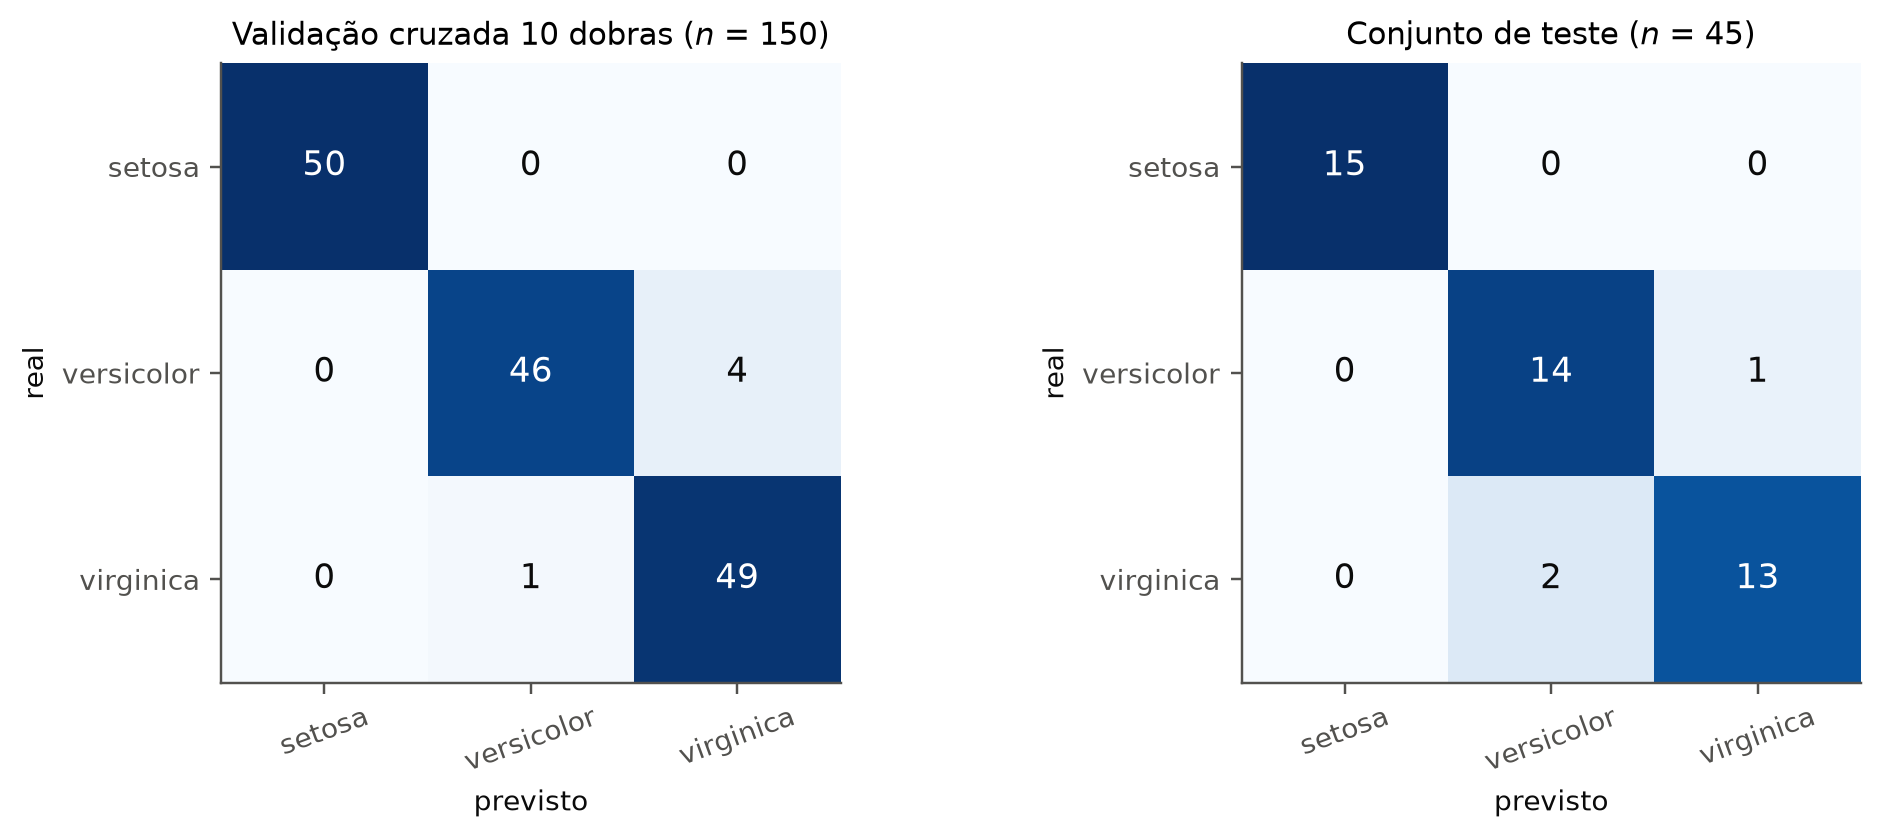
\includegraphics[width=\textwidth]{fig_confusao.png}
	\caption{Matrizes de confusão. À esquerda, previsões fora da amostra obtidas por validação
	cruzada de 10 dobras sobre as 150 amostras; à direita, o conjunto de teste de 45 amostras.}
	\label{fig:confusao}
\end{figure}

\subsection{Diagnóstico dos erros}

A matriz de confusão da validação cruzada (150 amostras) está na \tabela{tab:confusao}. Três
fatos se destacam.

\begin{table}[htbp]
	\centering
	\caption{Matriz de confusão da validação cruzada de 10 dobras (150 amostras). Linhas: classe
	real; colunas: classe prevista.}
	\label{tab:confusao}
	% gerado automaticamente por mlp_iris.py - nao editar

\begin{tabular}{lccc}
\toprule
\textbf{real $\backslash$ previsto} & \textbf{setosa} & \textbf{versicolor} & \textbf{virginica} \\
\midrule
setosa & 50 & 0 & 0 \\
versicolor & 0 & 46 & 4 \\
virginica & 0 & 1 & 49 \\
\bottomrule
\end{tabular}

\end{table}

\begin{enumerate}
	\item a \emph{setosa} é classificada perfeitamente: 50 de 50. Isso era esperado pela análise
	      exploratória, já que a classe é separável;
	\item os erros entre \emph{versicolor} e \emph{virginica} são assimétricos: quatro
	      \emph{versicolor} foram previstas como \emph{virginica} e apenas uma \emph{virginica} foi
	      prevista como \emph{versicolor}. O modelo erra mais na direção da classe de pétalas
	      maiores;
	\item não há confusão entre \emph{setosa} e qualquer outra classe, o que confirma que a rede
	      aprendeu a estrutura global antes de refinar a fronteira difícil.
\end{enumerate}

A \tabela{tab:por-classe} detalha precisão, revocação e $F_1$ por classe. A \emph{setosa} tem
$100\,\%$ nas três métricas. A \emph{versicolor} tem precisão alta ($97{,}9\,\%$) e revocação mais
baixa ($92{,}0\,\%$): quando o modelo diz \emph{versicolor}, quase sempre acerta, mas deixa passar
algumas. A \emph{virginica} mostra o padrão oposto: revocação de $98{,}0\,\%$ e precisão de
$92{,}5\,\%$.

\begin{table}[htbp]
	\centering
	\caption{Métricas por classe na validação cruzada de 10 dobras (\%).}
	\label{tab:por-classe}
	% gerado automaticamente por mlp_iris.py - nao editar

\begin{tabular}{lrrrr}
\toprule
\textbf{Classe} & \textbf{Suporte} & \textbf{Precisão} & \textbf{Revocação} & \textbf{F1} \\
\midrule
setosa & 50 & 100{,}0 & 100{,}0 & 100{,}0 \\
versicolor & 50 & 97{,}9 & 92{,}0 & 94{,}8 \\
virginica & 50 & 92{,}5 & 98{,}0 & 95{,}1 \\
\bottomrule
\end{tabular}

\end{table}

\begin{figure}[htbp]
	\centering
	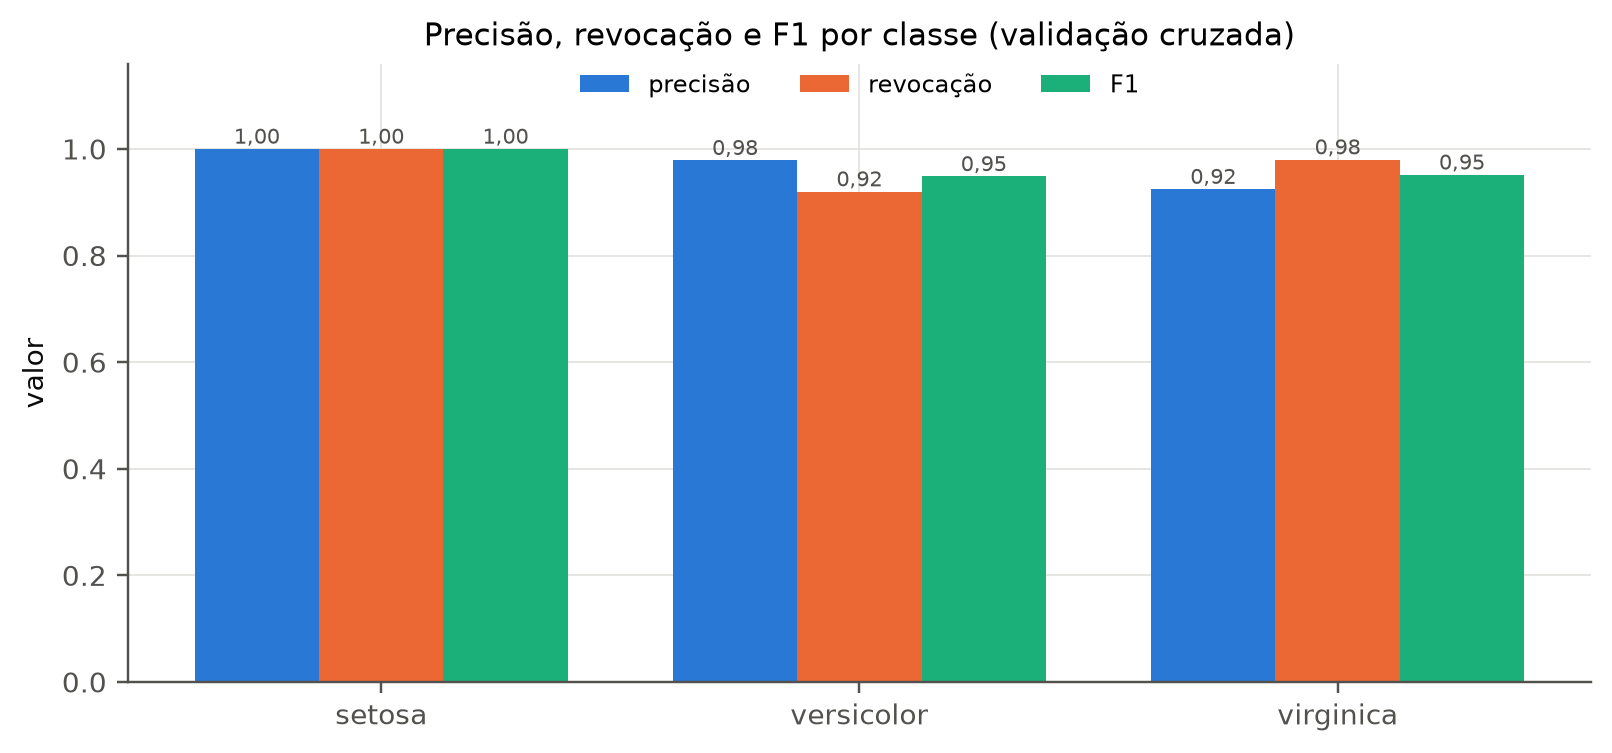
\includegraphics[width=0.78\textwidth]{fig_metricas_por_classe.png}
	\caption{Precisão, revocação e $F_1$ por classe na validação cruzada. O padrão assimétrico
	entre \emph{versicolor} e \emph{virginica} reflete a sobreposição das distribuições na
	fronteira.}
	\label{fig:metricas-classe}
\end{figure}

O padrão é coerente com a \figura{fig:dispersao}: as \emph{versicolor} com pétalas maiores
invadem a região da \emph{virginica}, e a rede, ao tentar separá-las, desloca a fronteira na
direção da \emph{versicolor}, errando mais para o lado da classe maior.

\subsection{Curva de treinamento}

A \figura{fig:curva-perda} mostra a evolução da perda e da acurácia de validação ao longo das
épocas, para o modelo treinado nos \nTreino{} exemplos. A perda cai de forma monotônica e suave,
sem oscilações bruscas --- sinal de que a taxa de aprendizado do Adam está adequada. A acurácia de
validação atinge $90{,}5\,\%$ e estagna; a parada antecipada interrompe o treinamento na época
\nIter{}, devolvendo os pesos da melhor época. A perda final é \perdaFinal{}.

\begin{figure}[htbp]
	\centering
	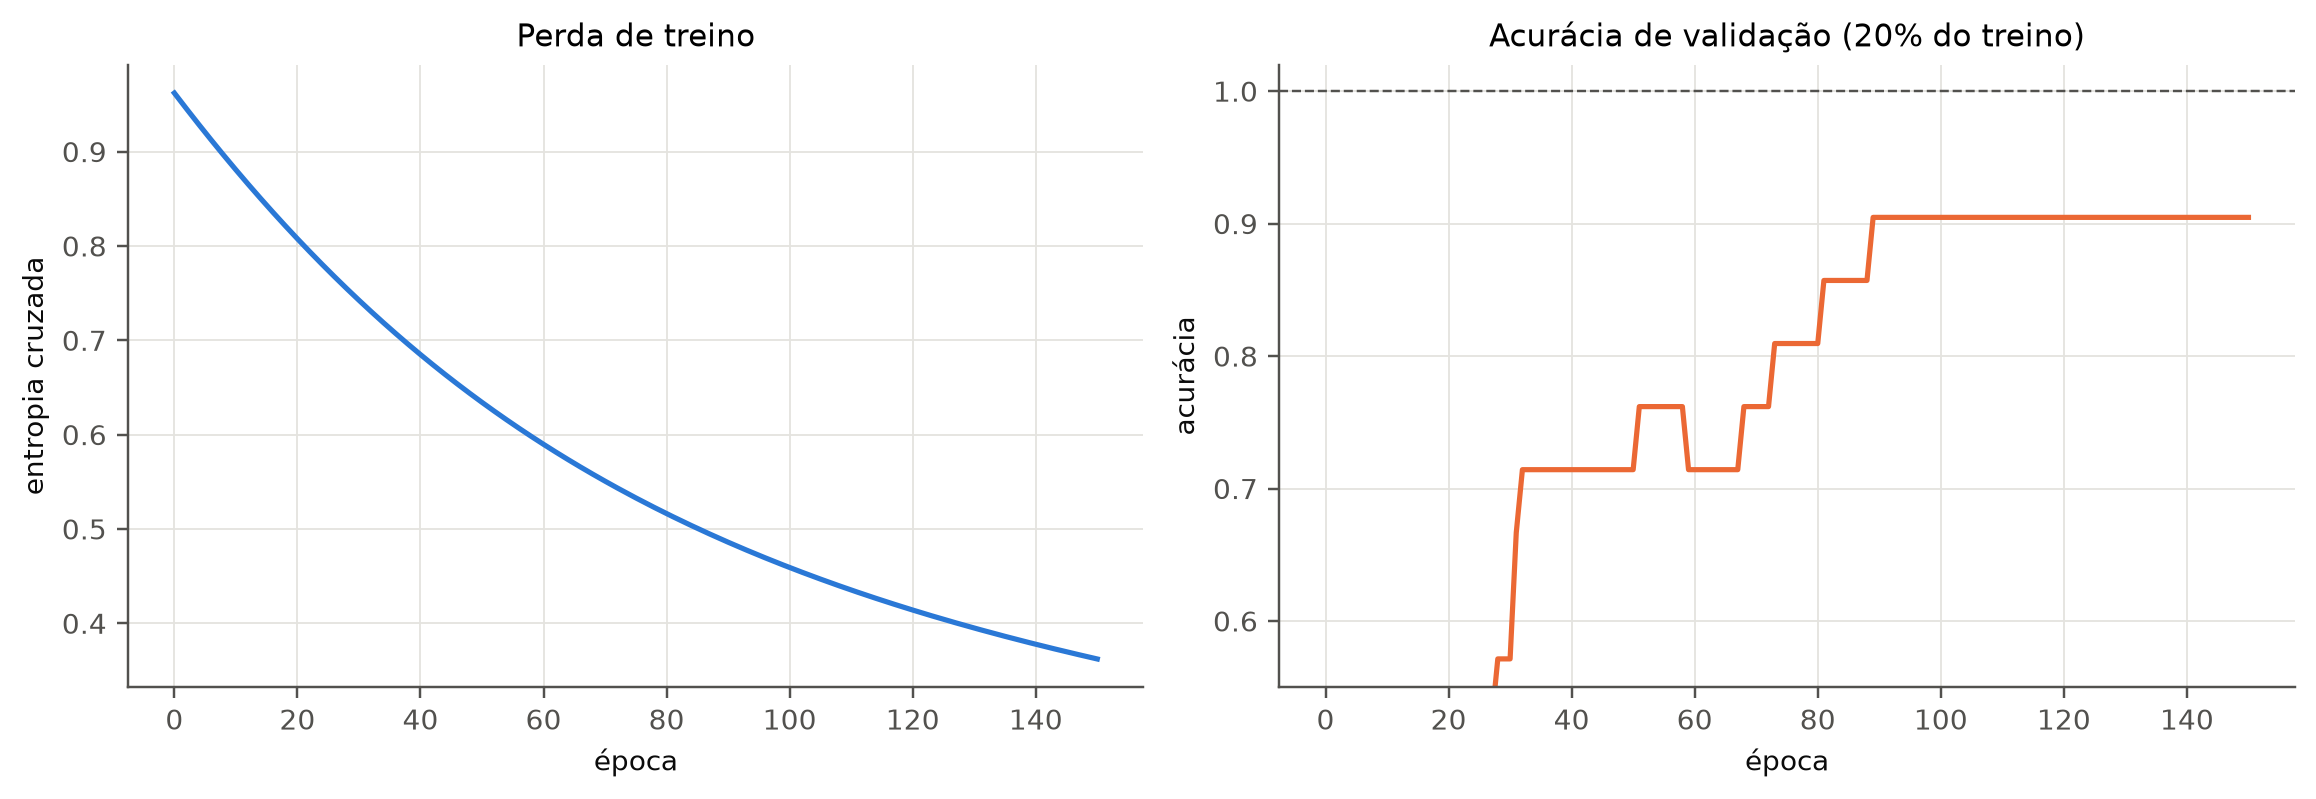
\includegraphics[width=\textwidth]{fig_curva_perda.png}
	\caption{Curva de treinamento: perda de treino (esquerda) e acurácia no conjunto de validação
	interno, 20\,\% do treino (direita). A linha tracejada marca $100\,\%$ de acerto.}
	\label{fig:curva-perda}
\end{figure}

Vale notar que a acurácia de validação interna é mais baixa que a acurácia de teste. Isso não é
paradoxo: o conjunto de validação interno tem apenas 21 amostras, e cada erro custa $4{,}8$ pontos
percentuais. A curva é útil para detectar overfitting e escolher a época de parada, não para
estimar o desempenho final.

\subsection{Curva de aprendizado}

A curva de aprendizado responde a uma pergunta prática: mais dados ajudariam? A
\figura{fig:curva-aprendizado} mostra a acurácia de treino e de validação em função do tamanho do
conjunto de treinamento, mantendo o teste fixo em uma dobra de cada vez.

\begin{figure}[htbp]
	\centering
	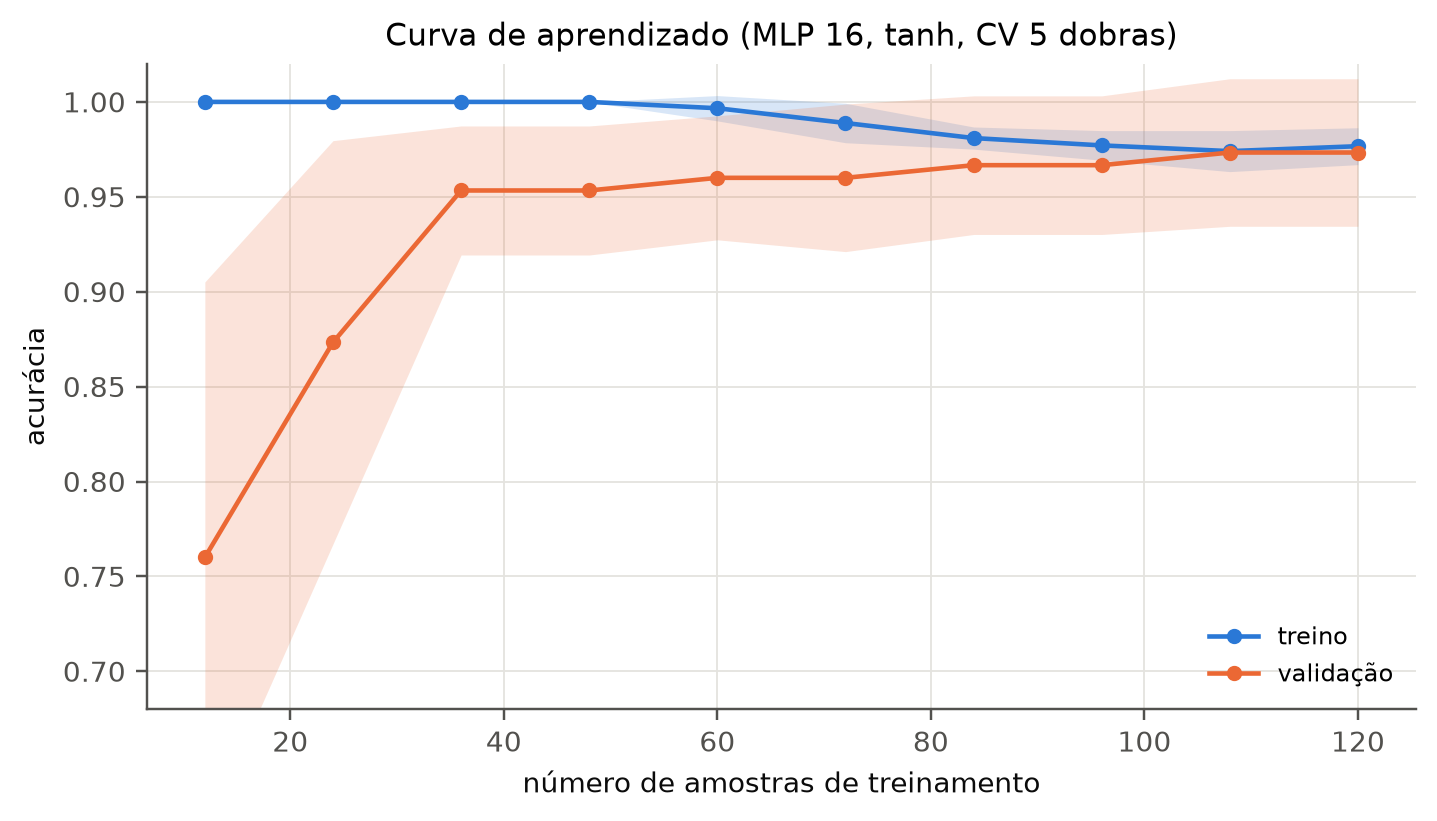
\includegraphics[width=0.78\textwidth]{fig_curva_aprendizado.png}
	\caption{Curva de aprendizado do modelo principal (validação cruzada de 5 dobras, 10 tamanhos
	de treino). A faixa sombreada representa $\pm 1$ desvio-padrão entre as dobras.}
	\label{fig:curva-aprendizado}
\end{figure}

Com 12 amostras de treino, a acurácia de validação é de apenas $76\,\%$ e a variabilidade é enorme.
Com 36 amostras, já chega a $95\,\%$. A partir daí, o ganho é marginal: com 120 amostras, a
validação chega a $97{,}3\,\%$. A curva de treino, por sua vez, cai ligeiramente de $100\,\%$ para
$97{,}7\,\%$ --- a rede deixa de decorar e passa a generalizar. O padrão indica que o problema está
mais limitado pela fronteira entre as classes do que pela quantidade de dados: a partir de ~40
amostras por classe, o retorno de coletar mais dados é pequeno.

\subsection{Efeito da arquitetura}

A \tabela{tab:arquiteturas} e a \figura{fig:arquiteturas} comparam nove arquiteturas, de um único
neurônio a duas camadas com $128$ e $64$ neurônios. O resultado é inequívoco: \emph{a arquitetura
quase não importa neste problema}. Todas as configurações ficam entre $94{,}7\,\%$ e
$96{,}7\,\%$, uma faixa de 2 pontos percentuais, enquanto o desvio entre dobras é de cerca de
$4$ pontos.

\begin{table}[htbp]
	\centering
	\caption{Acurácia por arquitetura (validação cruzada 5 dobras $\times$ 3 repetições). A coluna
	de parâmetros conta pesos e vieses.}
	\label{tab:arquiteturas}
	% gerado automaticamente por mlp_iris.py - nao editar

\begin{tabular}{lrrrrr}
\toprule
\textbf{arquitetura} & \textbf{profundidade} & \textbf{parâmetros} & \textbf{acurácia} & \textbf{desvio} & \textbf{log-loss} \\
\midrule
(4) & 1 & 35 & 96{,}7 & 4{,}0 & 0{,}171 \\
(8) & 1 & 67 & 95{,}3 & 3{,}5 & 0{,}112 \\
(16) & 1 & 131 & 94{,}7 & 4{,}1 & 0{,}104 \\
(32) & 1 & 259 & 94{,}9 & 4{,}0 & 0{,}103 \\
(8, 4) & 2 & 91 & 96{,}2 & 3{,}3 & 0{,}083 \\
(16, 8) & 2 & 243 & 95{,}3 & 3{,}7 & 0{,}096 \\
(32, 16) & 2 & 739 & 94{,}7 & 4{,}1 & 0{,}095 \\
(64, 32) & 2 & 2499 & 95{,}3 & 4{,}3 & 0{,}102 \\
(128, 64) & 2 & 9091 & 94{,}9 & 4{,}5 & 0{,}154 \\
\bottomrule
\end{tabular}

\end{table}

\begin{figure}[htbp]
	\centering
	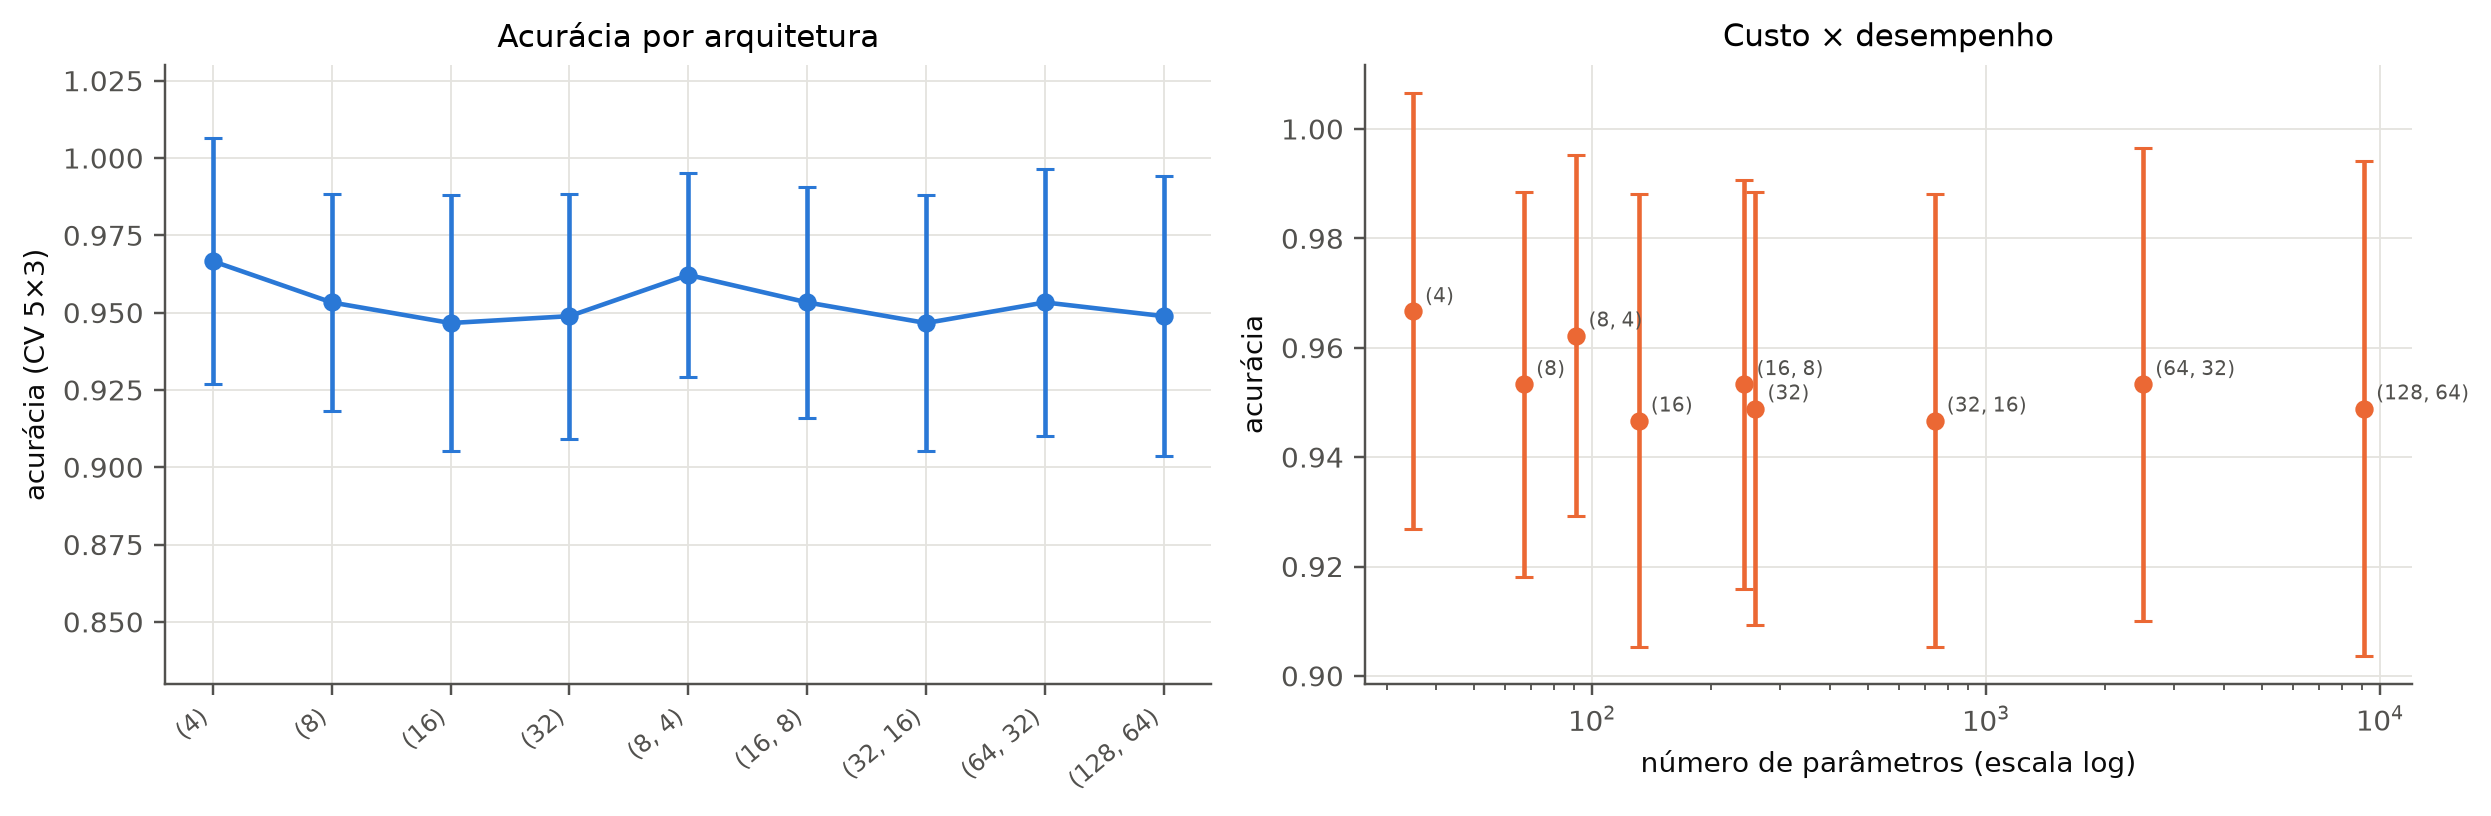
\includegraphics[width=\textwidth]{fig_arquiteturas.png}
	\caption{Acurácia por arquitetura (esquerda) e relação entre número de parâmetros e acurácia
	(direita, escala logarítmica). As barras de erro são $\pm 1$ desvio-padrão entre as 15 dobras.}
	\label{fig:arquiteturas}
\end{figure}

Dois pontos merecem comentário. Primeiro, a melhor configuração é a menor: um único neurônio
oculto com 4 unidades ($96{,}7\,\%$, 35 parâmetros). Segundo, as redes maiores não melhoram ---
pioram ligeiramente. A rede com $128$ e $64$ neurônios tem 9\,091 parâmetros para 150 amostras,
uma razão de 60 parâmetros por amostra, e sua acurácia cai para $94{,}9\,\%$ com o maior desvio de
todas as configurações. É o retrato clássico do excesso de capacidade: o modelo tem liberdade para
ajustar ruído.

Esse resultado não significa que arquiteturas maiores sejam inúteis; significa que, \emph{neste
problema}, a informação está em duas dimensões efetivas e uma fronteira simples basta. A
\figura{fig:fronteira-capacidade} mostra exatamente isso: as fronteiras de decisão de redes com 2,
4, 24 e 112 neurônios são visualmente quase idênticas.

\subsection{Efeito da função de ativação}

A \tabela{tab:ativacoes} compara quatro ativações com a mesma arquitetura $(16,8)$. A
\emph{tanh} e a logística lideram ($96{,}2\,\%$), a ReLU fica em $95{,}3\,\%$ e a identidade em
$96{,}0\,\%$. As diferenças estão dentro de um desvio-padrão e não devem ser interpretadas como
superioridade de uma função sobre outra.

\begin{table}[htbp]
	\centering
	\caption{Efeito da função de ativação na camada oculta (arquitetura $(16,8)$,
	validação cruzada 5 $\times$ 3).}
	\label{tab:ativacoes}
	% gerado automaticamente por mlp_iris.py - nao editar

\begin{tabular}{lrrr}
\toprule
\textbf{ativação} & \textbf{acurácia} & \textbf{desvio} & \textbf{log-loss} \\
\midrule
relu & 95{,}3 & 3{,}7 & 0{,}096 \\
tanh & 96{,}2 & 3{,}3 & 0{,}095 \\
logistic & 96{,}2 & 3{,}3 & 0{,}106 \\
identity & 96{,}0 & 3{,}4 & 0{,}083 \\
\bottomrule
\end{tabular}

\end{table}

\begin{figure}[htbp]
	\centering
	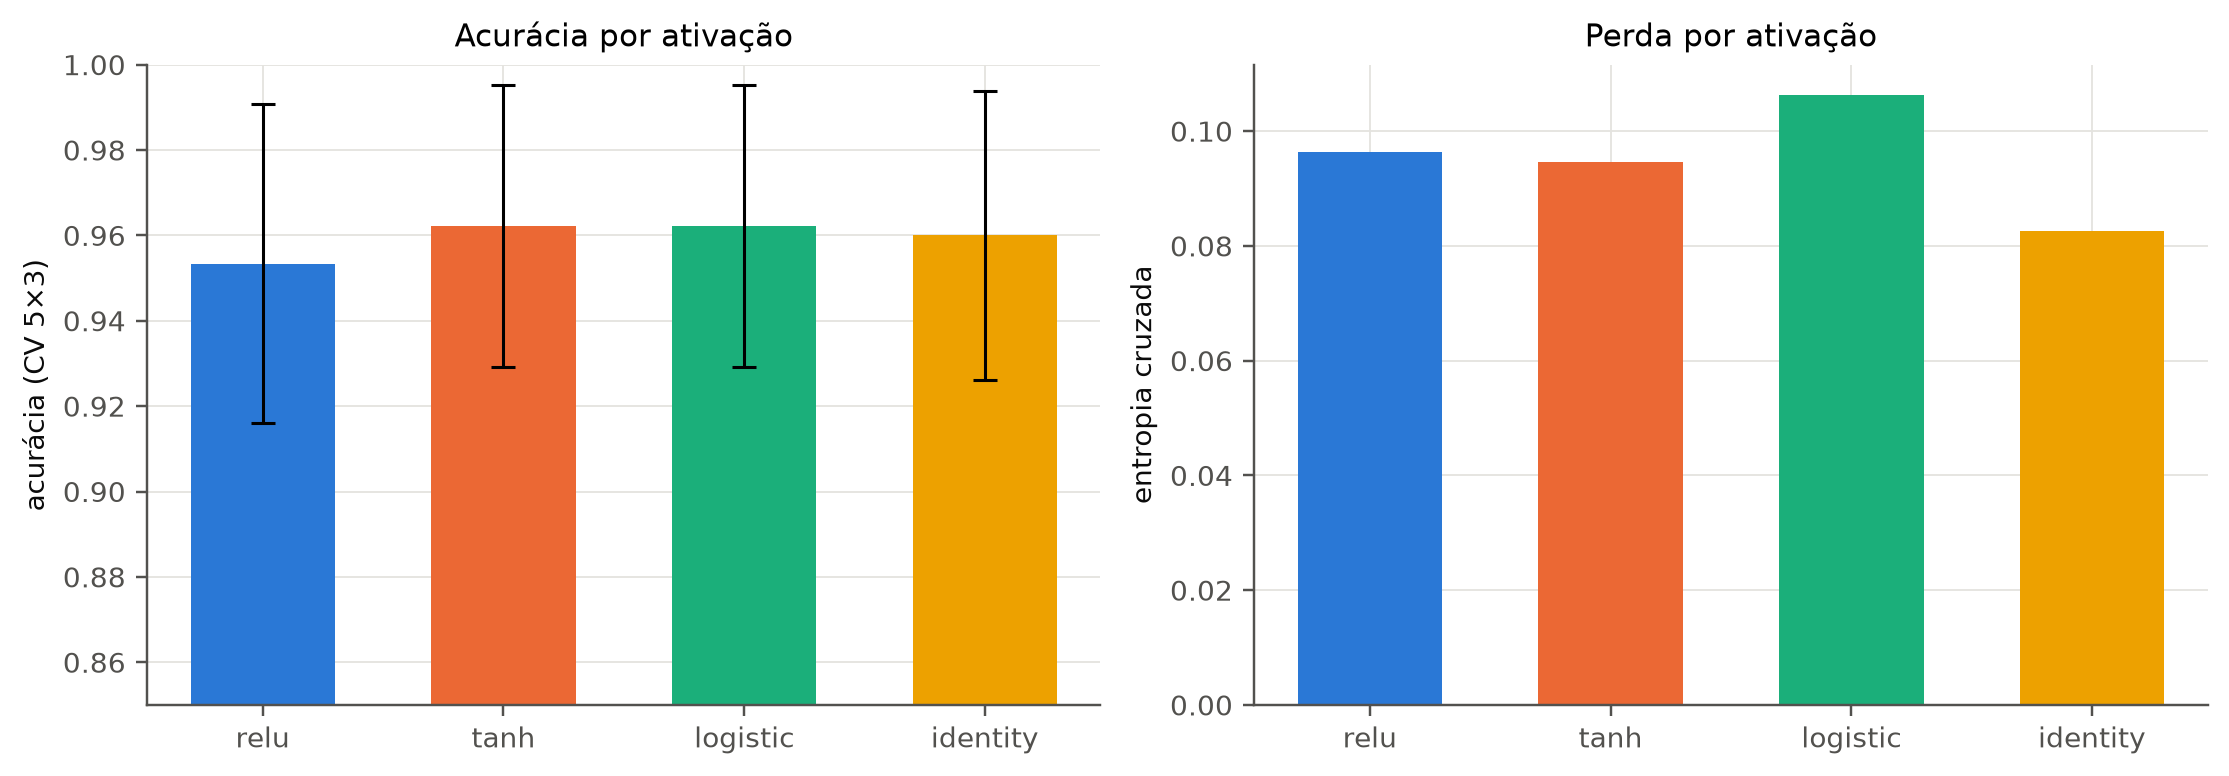
\includegraphics[width=\textwidth]{fig_ativacoes.png}
	\caption{Acurácia e entropia cruzada por função de ativação. A identidade, que torna a rede
	um modelo linear, tem a menor entropia cruzada --- evidência de que o problema é quase
	linearmente separável.}
	\label{fig:ativacoes}
\end{figure}

O detalhe mais informativo está na coluna de entropia cruzada: a \emph{identidade} tem a menor
perda ($0{,}083$), seguida de perto por \emph{tanh} ($0{,}095$) e ReLU ($0{,}096$). Uma rede sem
não linearidade na camada oculta produz a melhor calibração de probabilidades. Isso é uma pista
forte de que a fronteira entre as classes é essencialmente linear e que a não linearidade não está
sendo usada para melhorar a separação --- apenas para ajustar detalhes.

\subsection{Efeito da regularização}

A \figura{fig:regularizacao} varre $\alpha$ de $10^{-6}$ a $10^{2}$ em escala logarítmica, com a
arquitetura $(32,16)$. O comportamento tem três regimes bem definidos:

\begin{itemize}
	\item \textbf{$\alpha \lesssim 1$}: acurácia praticamente constante em torno de $95$--$96\,\%$ e
	      entropia cruzada mínima. A regularização é fraca demais para ter efeito;
	\item \textbf{$\alpha \approx 1$}: a entropia cruzada atinge o mínimo ($0{,}089$). É o ponto em
	      que a penalidade começa a estabilizar as probabilidades;
	\item \textbf{$\alpha \gtrsim 10$}: colapso. Com $\alpha = 10$, a acurácia cai para
	      $89\,\%$; com $\alpha = 100$, para $33\,\%$ --- o modelo prevê uma única classe para
	      todas as amostras, porque a penalidade domina a perda e os pesos vão a zero.
\end{itemize}

\begin{figure}[htbp]
	\centering
	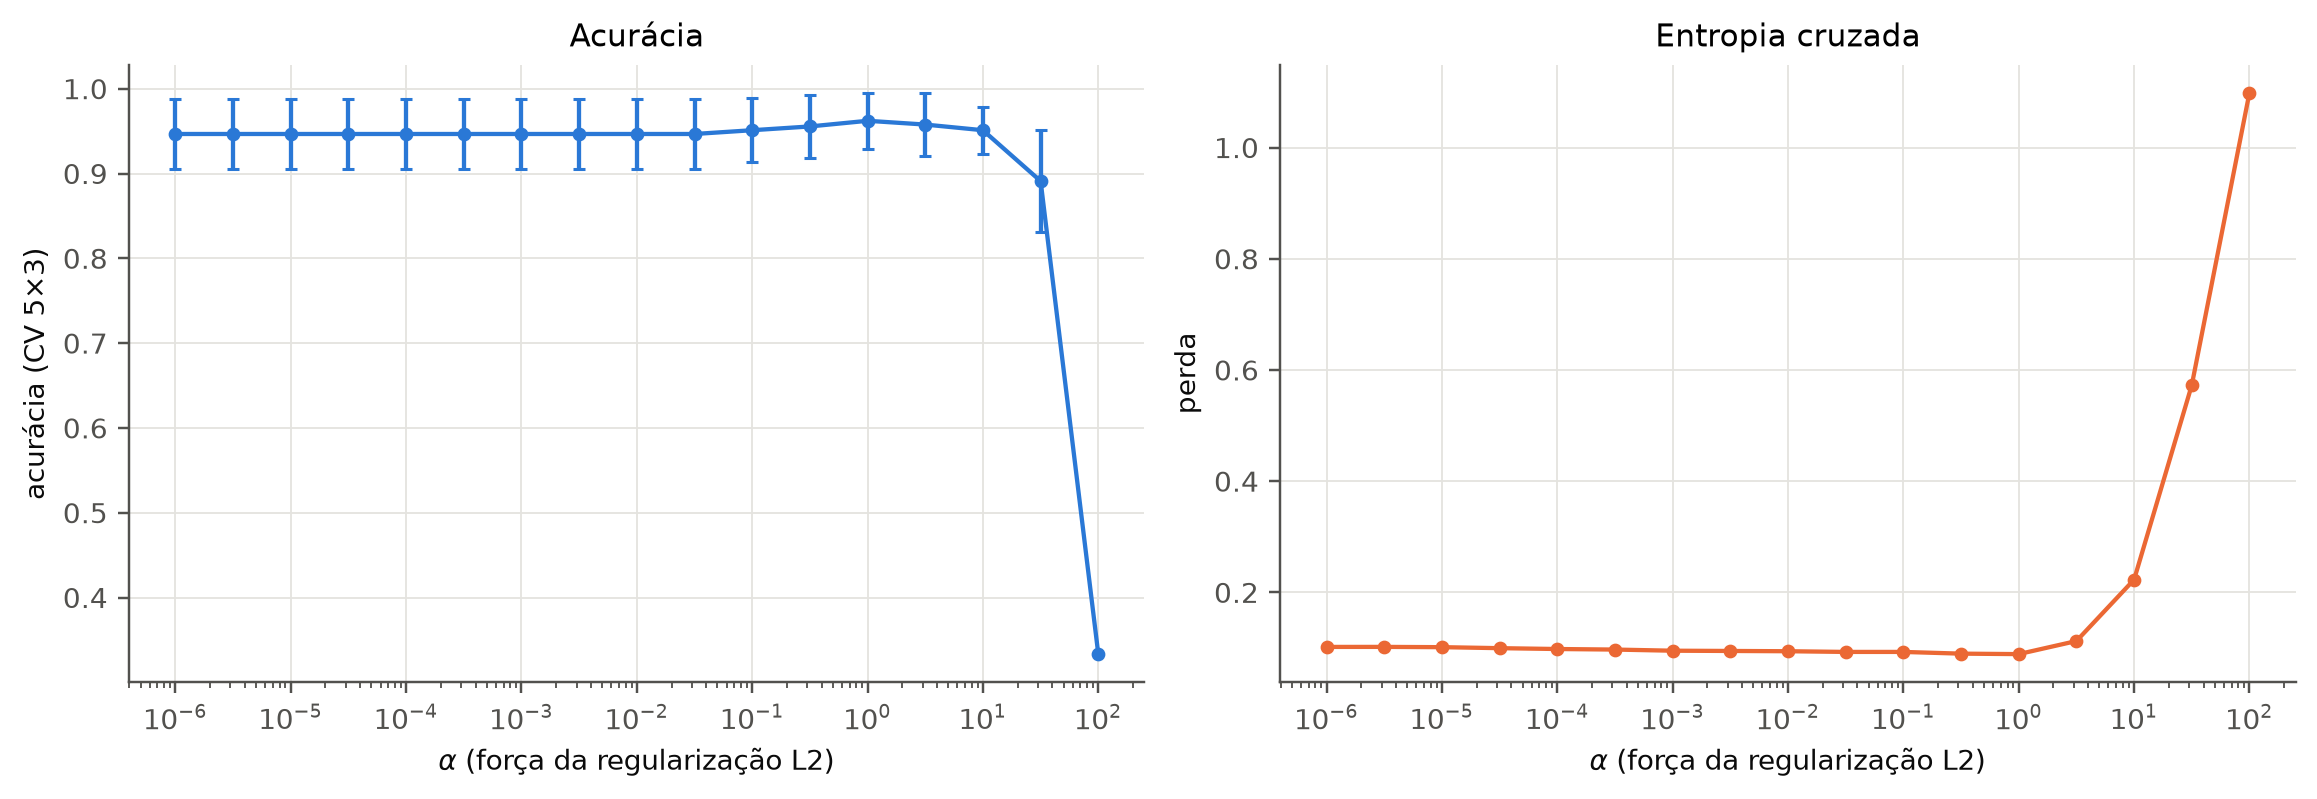
\includegraphics[width=\textwidth]{fig_regularizacao.png}
	\caption{Efeito da força de regularização $L_2$ na acurácia e na entropia cruzada
	(arquitetura $(32,16)$, validação cruzada 5 $\times$ 3).}
	\label{fig:regularizacao}
\end{figure}

A lição prática é que existe uma faixa larga de valores seguros e um penhasco abrupto. Para um
problema pequeno como o Iris, qualquer $\alpha$ entre $10^{-4}$ e $10^{-1}$ funciona; a escolha de
$10^{-2}$ está confortavelmente no meio dessa faixa.

\subsection{Efeito da taxa de aprendizado}

A \figura{fig:taxas} mostra o treinamento com SGD e momento para cinco taxas iniciais. Os
resultados resumem o que se espera de um otimizador de primeira ordem:

\begin{itemize}
	\item $\eta_0 = 10^{-3}$: a perda mal se move em 300 épocas ($0{,}73$) e a acurácia de treino
	      fica em $68\,\%$. A taxa é pequena demais;
	\item $\eta_0 = 10^{-2}$: convergência lenta, mas estável ($0{,}082$);
	\item $\eta_0 = 5\times10^{-2}$ e $10^{-1}$: convergência rápida e perda final baixa
	      ($0{,}041$ e $0{,}039$), com acurácia de treino de $98{,}7\,\%$;
	\item $\eta_0 = 5\times10^{-1}$: a perda despenca e depois oscila; a acurácia final cai para
	      $98\,\%$. A taxa é grande demais e o otimizador não se estabiliza.
\end{itemize}

\begin{figure}[htbp]
	\centering
	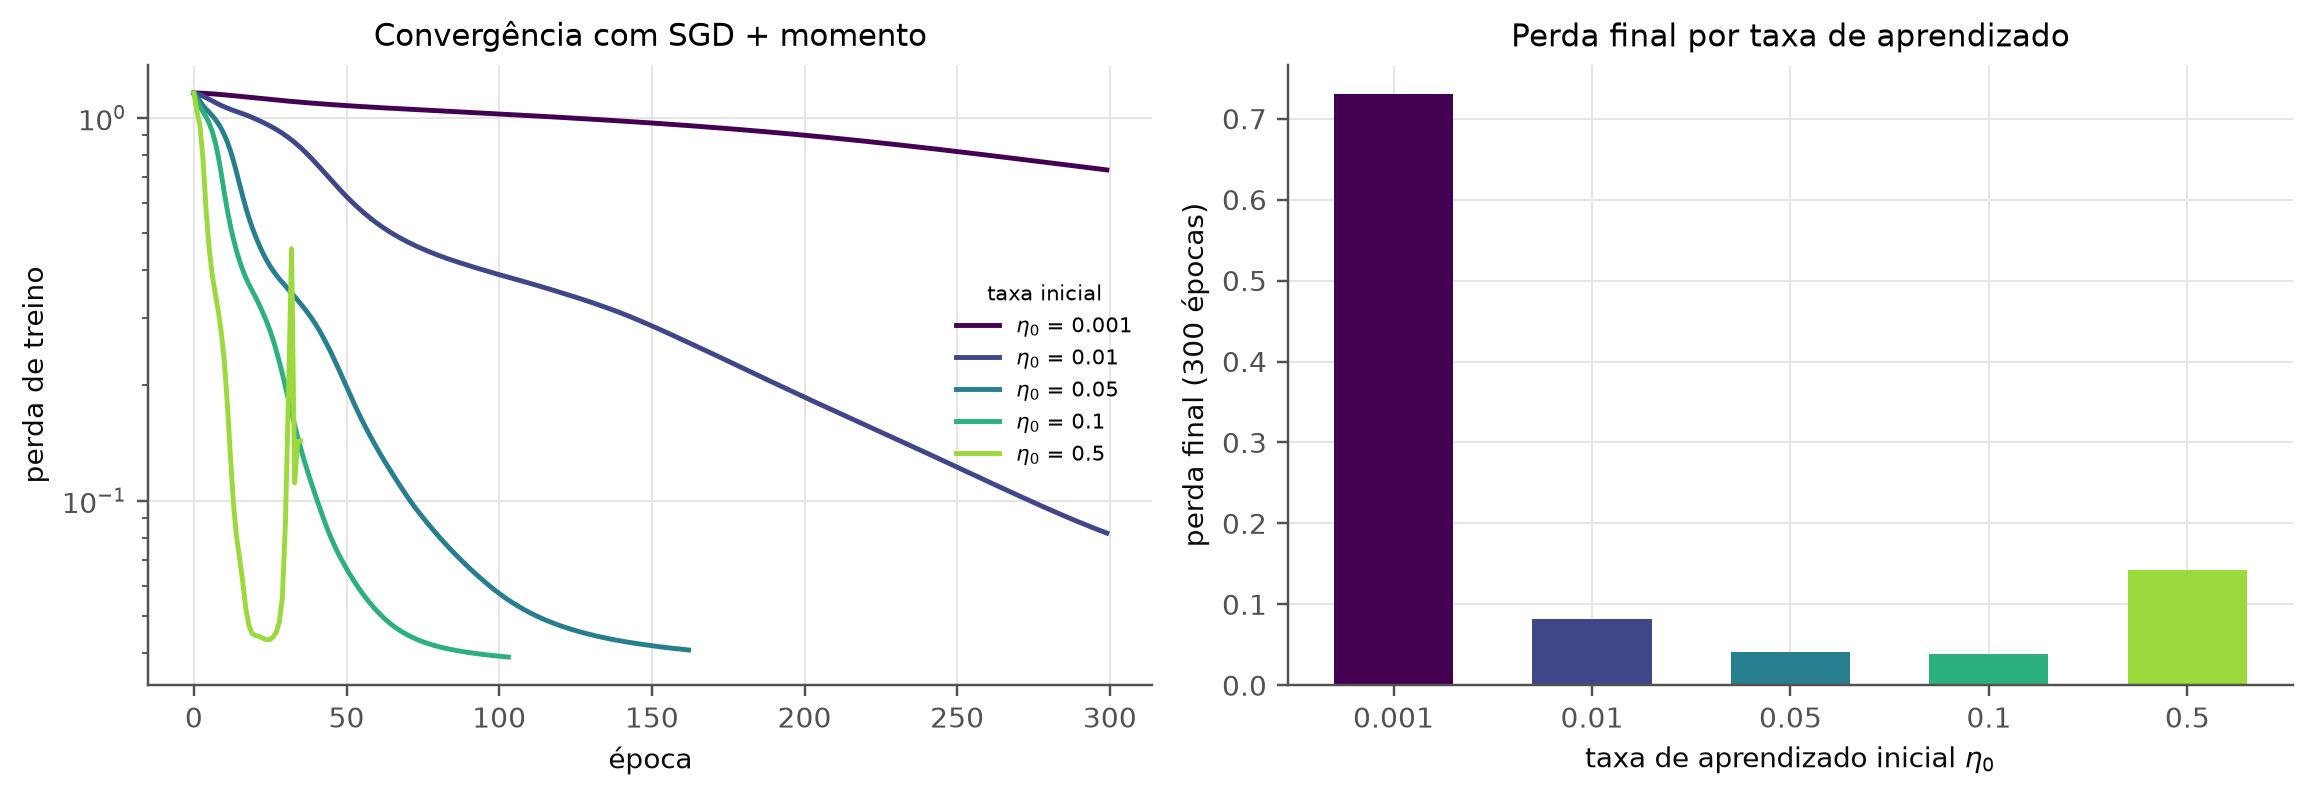
\includegraphics[width=\textwidth]{fig_taxas_aprendizado.png}
	\caption{Convergência do SGD com momento para diferentes taxas iniciais. À esquerda, perda de
	treino em escala logarítmica; à direita, perda final após 300 épocas.}
	\label{fig:taxas}
\end{figure}

A faixa útil vai de $10^{-2}$ a $10^{-1}$. O Adam, usado no modelo final, é mais tolerante: por
normalizar o passo por parâmetro, aceita taxas maiores sem divergir, e o padrão $10^{-3}$ do
scikit-learn foi suficiente.

\subsection{Fronteiras de decisão}

Para visualizar o que a rede aprendeu, a \figura{fig:fronteira-comparacao} treina quatro modelos
usando apenas comprimento e largura da pétala --- as duas variáveis mais informativas --- e mostra
as regiões de decisão no plano.

\begin{figure}[htbp]
	\centering
	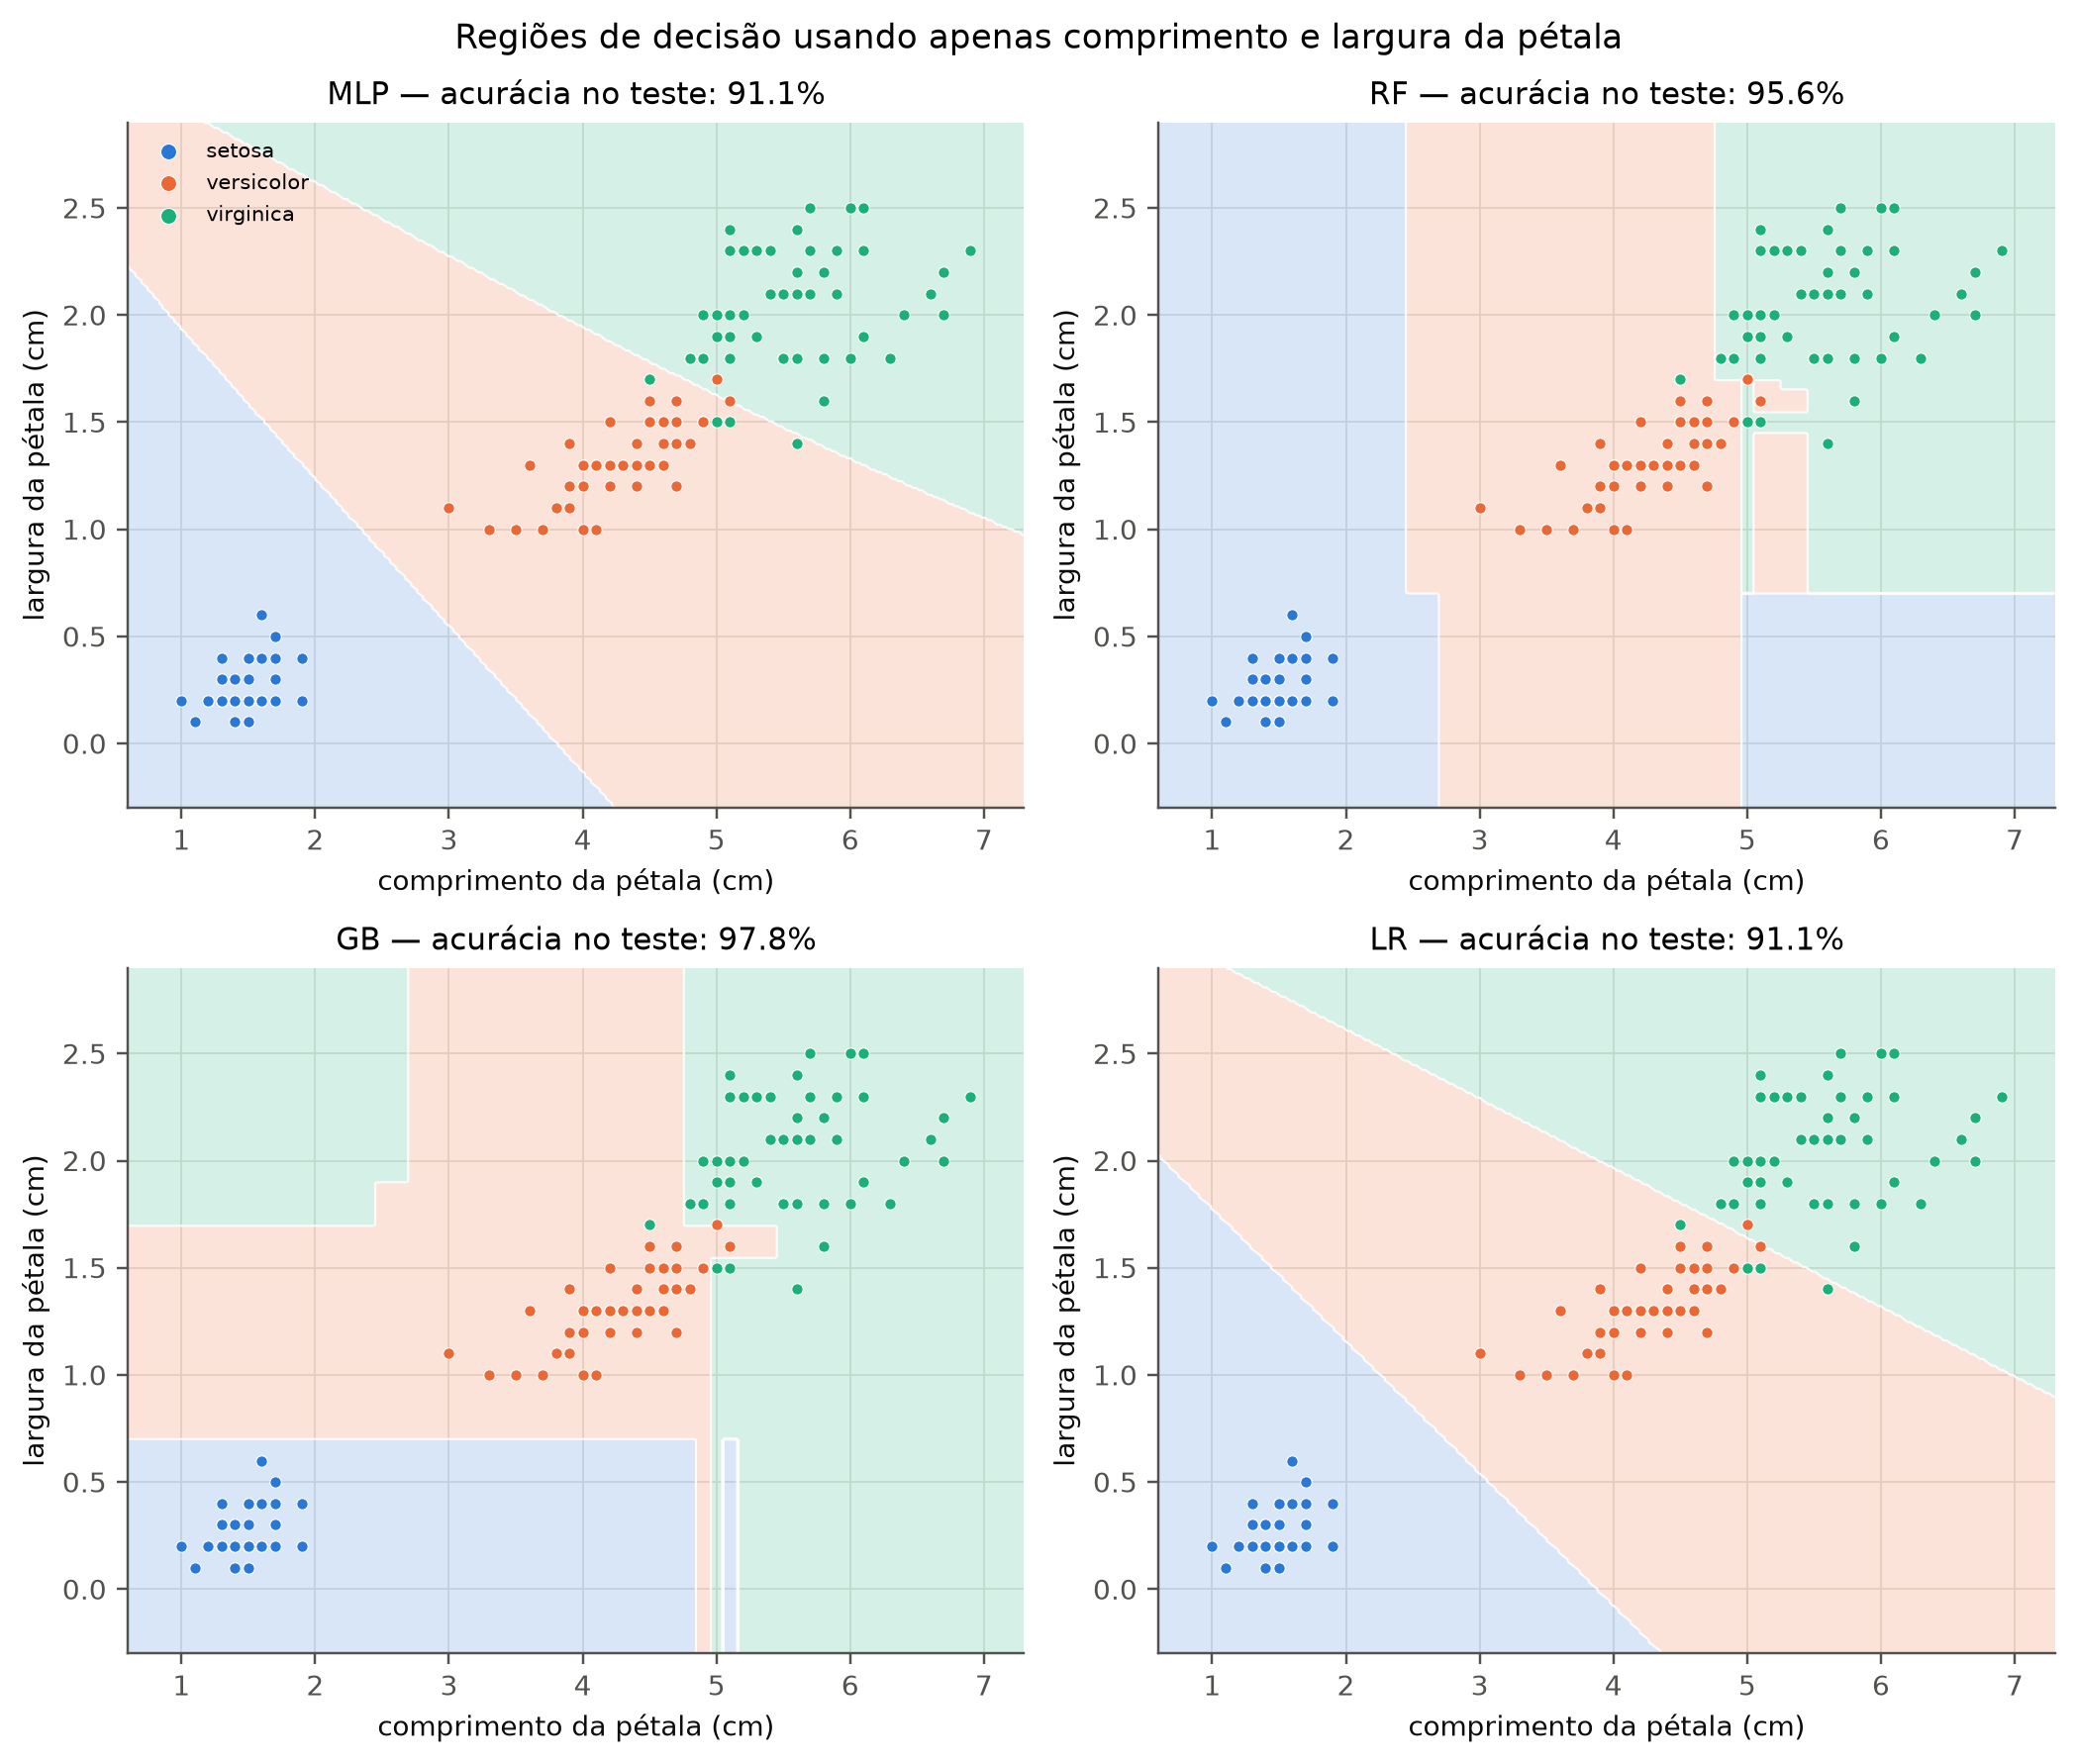
\includegraphics[width=0.95\textwidth]{fig_fronteira_comparacao.png}
	\caption{Regiões de decisão no plano da pétala para MLP, floresta aleatória, \emph{gradient
	boosting} e regressão logística. Cada modelo foi treinado apenas com os dois atributos
	mostrados; a acurácia indicada é a do conjunto de teste com esses dois atributos.}
	\label{fig:fronteira-comparacao}
\end{figure}

O resultado é revelador. A MLP produz duas fronteiras praticamente retas, assim como a regressão
logística. A floresta aleatória produz uma escada de retângulos, e o \emph{gradient boosting}
produz uma fronteira irregular que se ajusta a pontos individuais. Apesar das formas tão
diferentes, as acurácias são próximas: $91{,}1\,\%$ para MLP e regressão logística,
$95{,}6\,\%$ para a floresta e $97{,}8\,\%$ para o \emph{boosting}.

A semelhança entre MLP e regressão logística é a confirmação visual do que a entropia cruzada da
\tabela{tab:ativacoes} já sugeria: com duas variáveis e classes quase separáveis por uma reta, a
não linearidade da rede não encontra estrutura curva para explorar.

A \figura{fig:fronteira-capacidade} repete o exercício para redes de capacidade crescente. Mesmo
com 112 neurônios em três camadas, a fronteira permanece quase linear. A rede tem capacidade para
curvas muito mais complexas, mas os dados não pedem isso --- e a regularização $L_2$ desencoraja o
ajuste fino.

\begin{figure}[htbp]
	\centering
	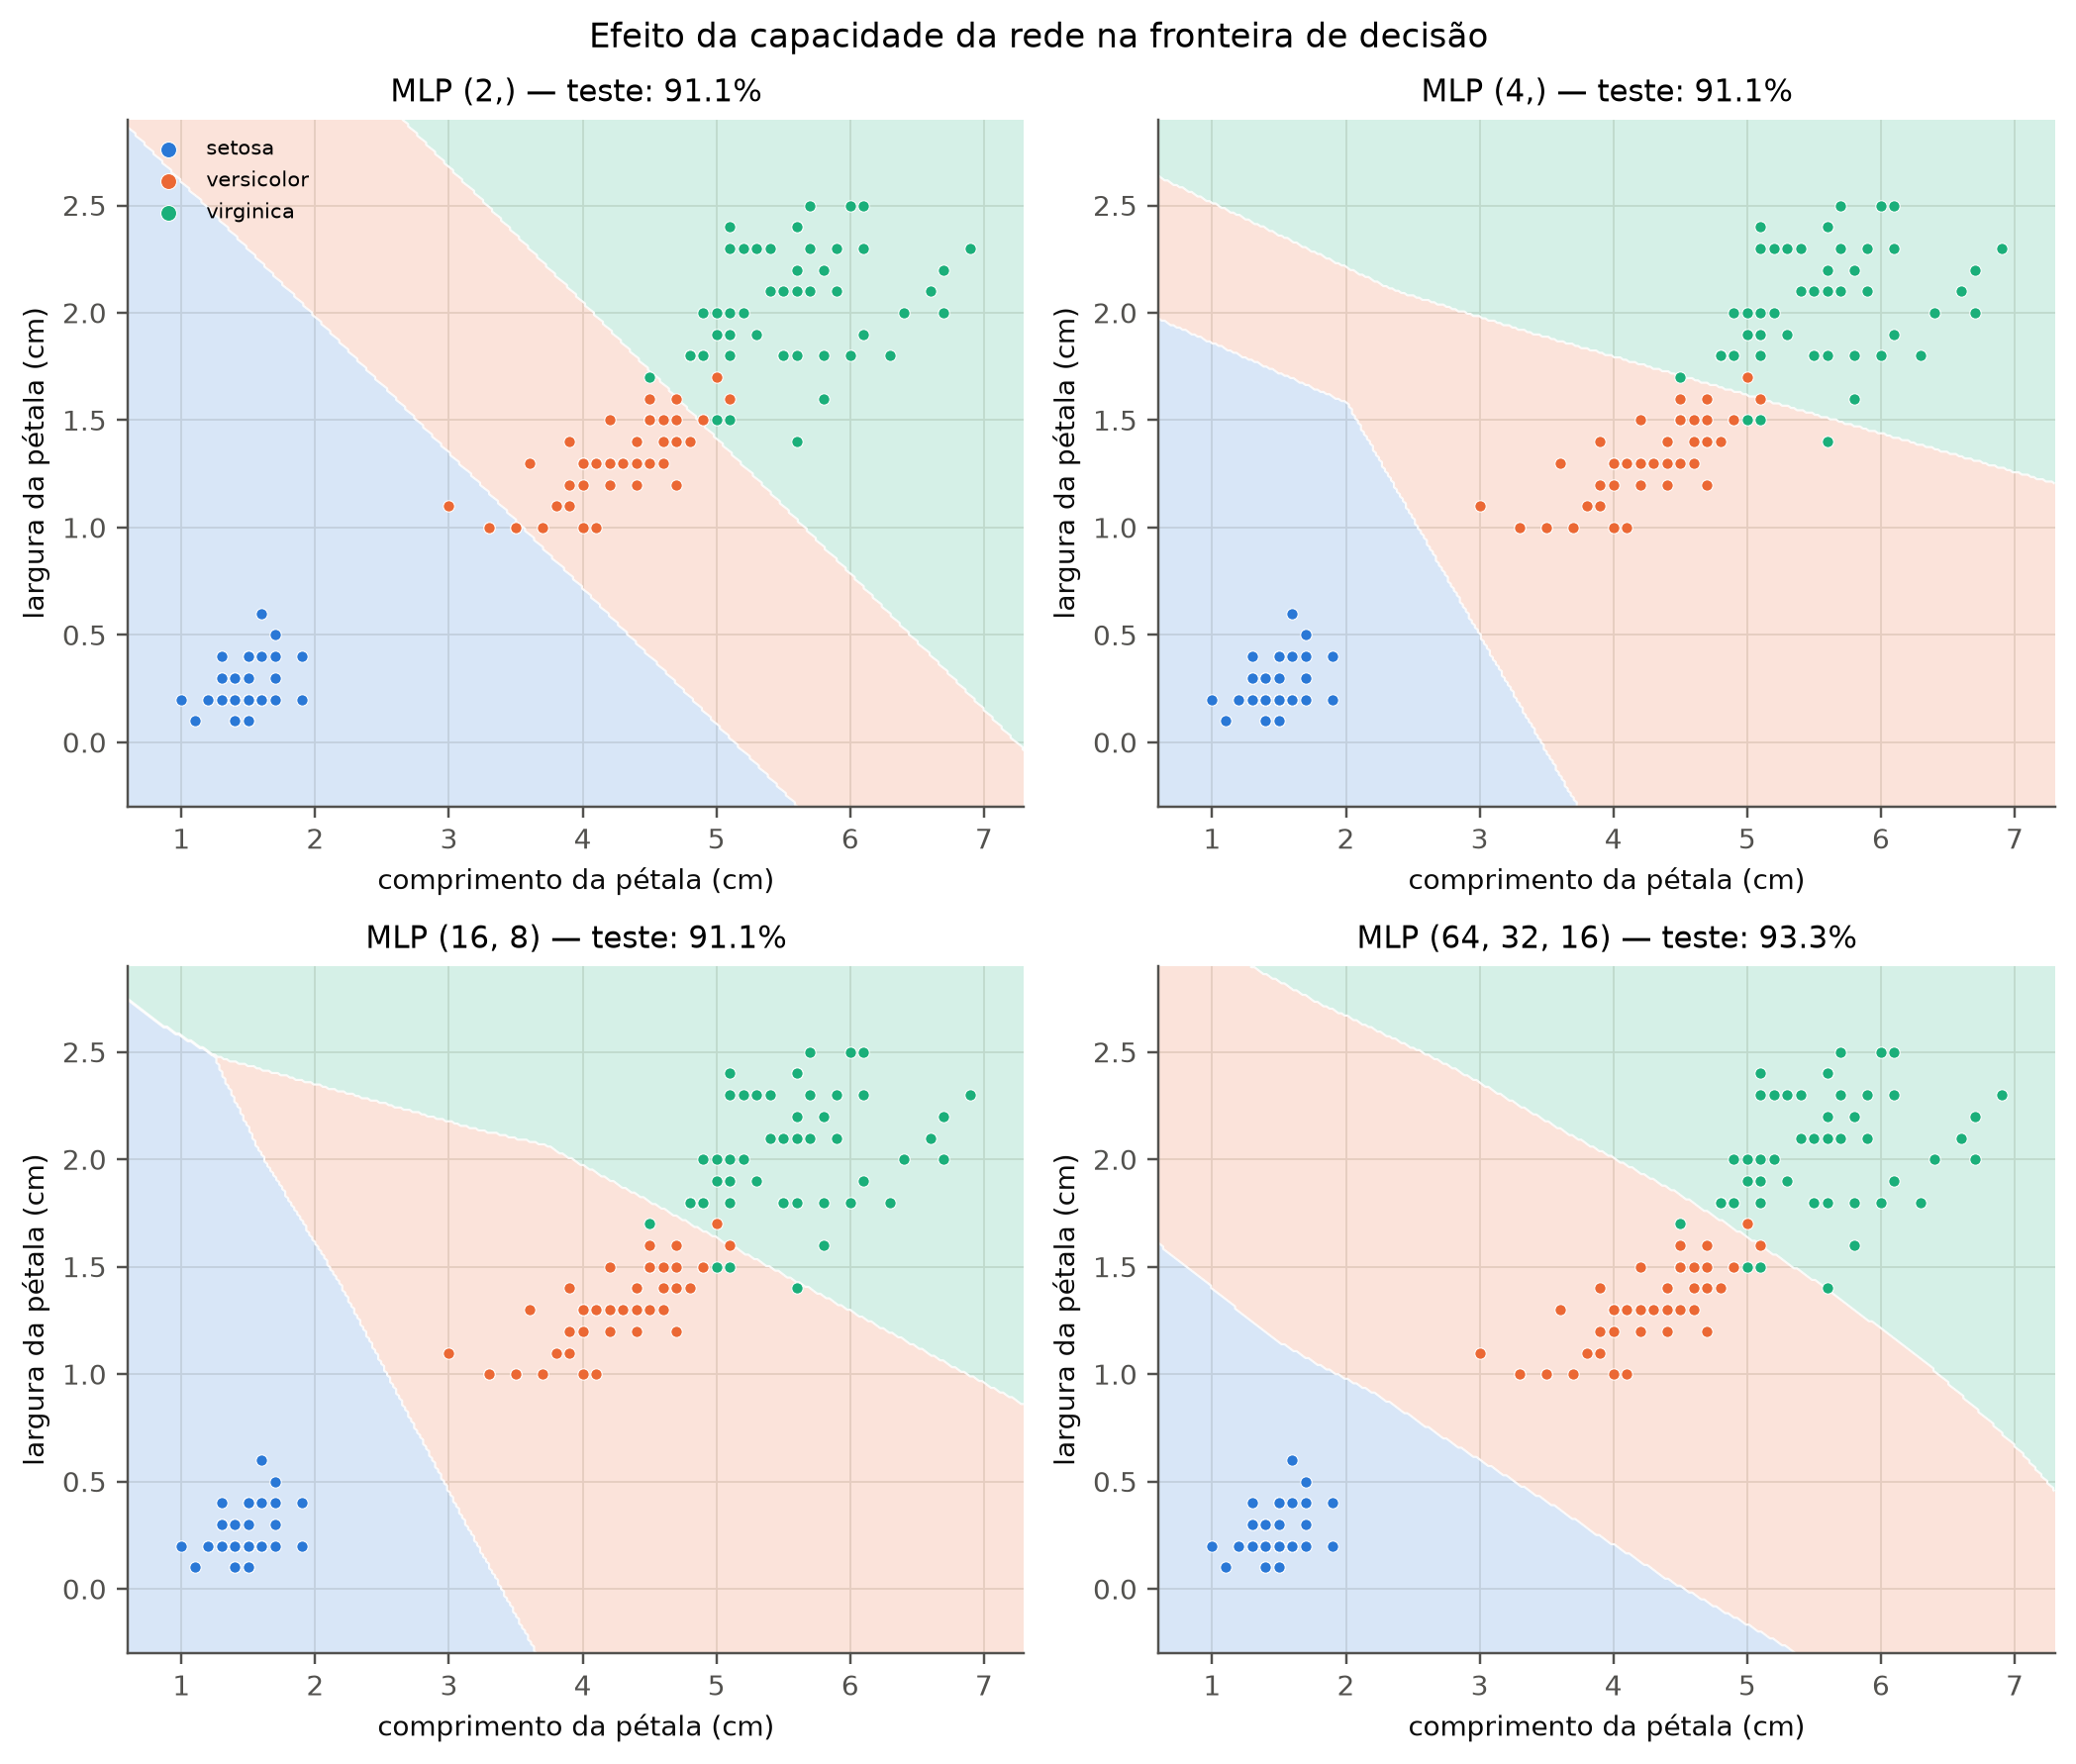
\includegraphics[width=0.95\textwidth]{fig_fronteira_capacidade.png}
	\caption{Fronteira de decisão para quatro capacidades, com os mesmos dois atributos. O aumento
	da capacidade não produz fronteiras mais complexas porque o problema é quase linearmente
	separável.}
	\label{fig:fronteira-capacidade}
\end{figure}

\subsection{Importância dos atributos}

A importância por permutação mede quanto a acurácia cai quando um atributo é embaralhado,
destruindo sua relação com a resposta. A \figura{fig:importancia} mostra o resultado para o
modelo de quatro atributos, no conjunto de teste, com 40 repetições.

\begin{figure}[htbp]
	\centering
	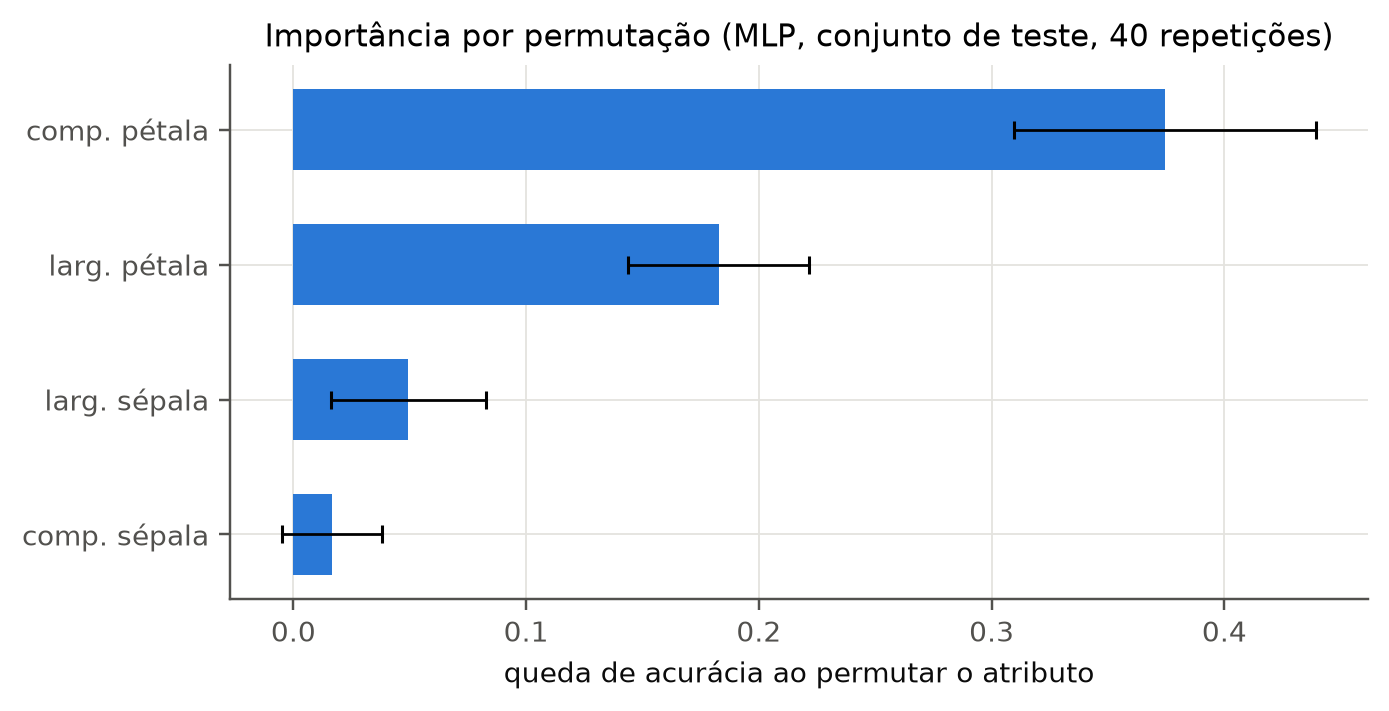
\includegraphics[width=0.72\textwidth]{fig_importancia.png}
	\caption{Importância por permutação no conjunto de teste (MLP de quatro atributos, 40
	repetições). A barra de erro é o desvio-padrão entre repetições.}
	\label{fig:importancia}
\end{figure}

O comprimento da pétala domina, com queda média de $37{,}4$ pontos percentuais. A largura da
pétala vem em segundo lugar ($18{,}3$), seguida pela largura da sépala ($4{,}9$) e pelo
comprimento da sépala ($1{,}7$). A hierarquia coincide com a análise exploratória: a pétala carrega
quase toda a informação discriminante, e a sépala contribui pouco.

Vale registrar uma limitação do método: quando dois atributos são muito correlacionados, permutar
um deles tem efeito pequeno, porque o outro carrega informação semelhante. Comprimento e largura
da pétala têm correlação de $0{,}96$; parte da importância de um é ``emprestada'' do outro. A
conclusão segura é que a pétala é o grupo informativo, não que o comprimento seja exatamente $7$
vezes mais importante que a largura.

\subsection{O que a rede aprendeu}

A \figura{fig:pesos} abre a caixa-preta: mostra as matrizes de pesos de uma rede compacta com 8
neurônios ocultos, treinada em todos os dados.

\begin{figure}[htbp]
	\centering
	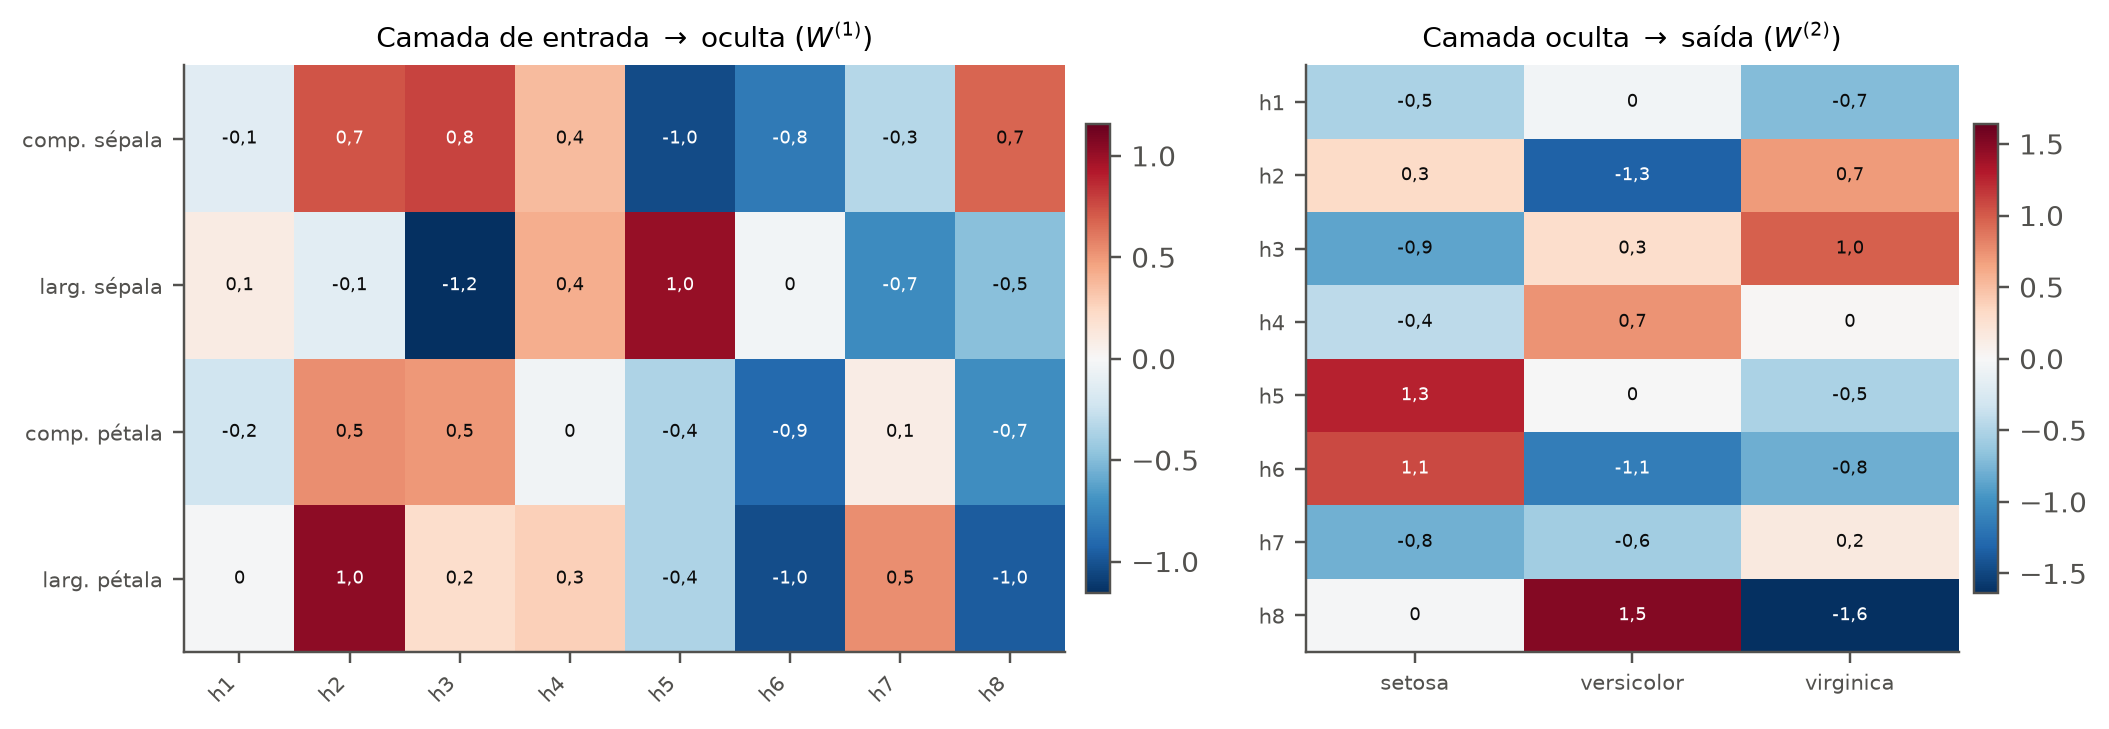
\includegraphics[width=\textwidth]{fig_pesos.png}
	\caption{Pesos aprendidos por uma rede $4$--$8$--$3$. À esquerda, $W^{(1)}$: quanto cada
	atributo pesa em cada neurônio oculto. À direita, $W^{(2)}$: quanto cada neurônio oculto
	contribui para cada classe. Azul é peso negativo, vermelho, positivo.}
	\label{fig:pesos}
\end{figure}

Alguns padrões são interpretáveis. Os neurônios $h_5$ e $h_6$ recebem peso positivo forte da
largura da pétala e do comprimento da pétala, e projetam-se de forma oposta em \emph{setosa} e
\emph{virginica} --- são detectores de ``pétala grande''. O neurônio $h_2$ tem peso positivo no
comprimento da sépala, mas não na pétala, e contribui negativamente para \emph{setosa}: captura a
sépala alongada que caracteriza as espécies maiores. Os demais neurônios combinam atributos de
forma menos óbvia, o que é esperado: a rede distribui a representação por várias unidades
redundantes.

O ponto didático é que a interpretabilidade não é automática. Os pesos são legíveis, mas a
``explicação'' só emerge quando combinados com a análise de importância e com o conhecimento do
problema. Em redes maiores, essa leitura direta deixa de ser viável e recorre-se a métodos
post-hoc.

\subsection{Comparação com modelos de referência}

A \tabela{tab:modelos} e a \figura{fig:comparacao} colocam a MLP ao lado de três alternativas, com
as mesmas dobras: floresta aleatória (400 árvores), \emph{gradient boosting} (300 estimadores) e
regressão logística multinomial.

\begin{figure}[htbp]
	\centering
	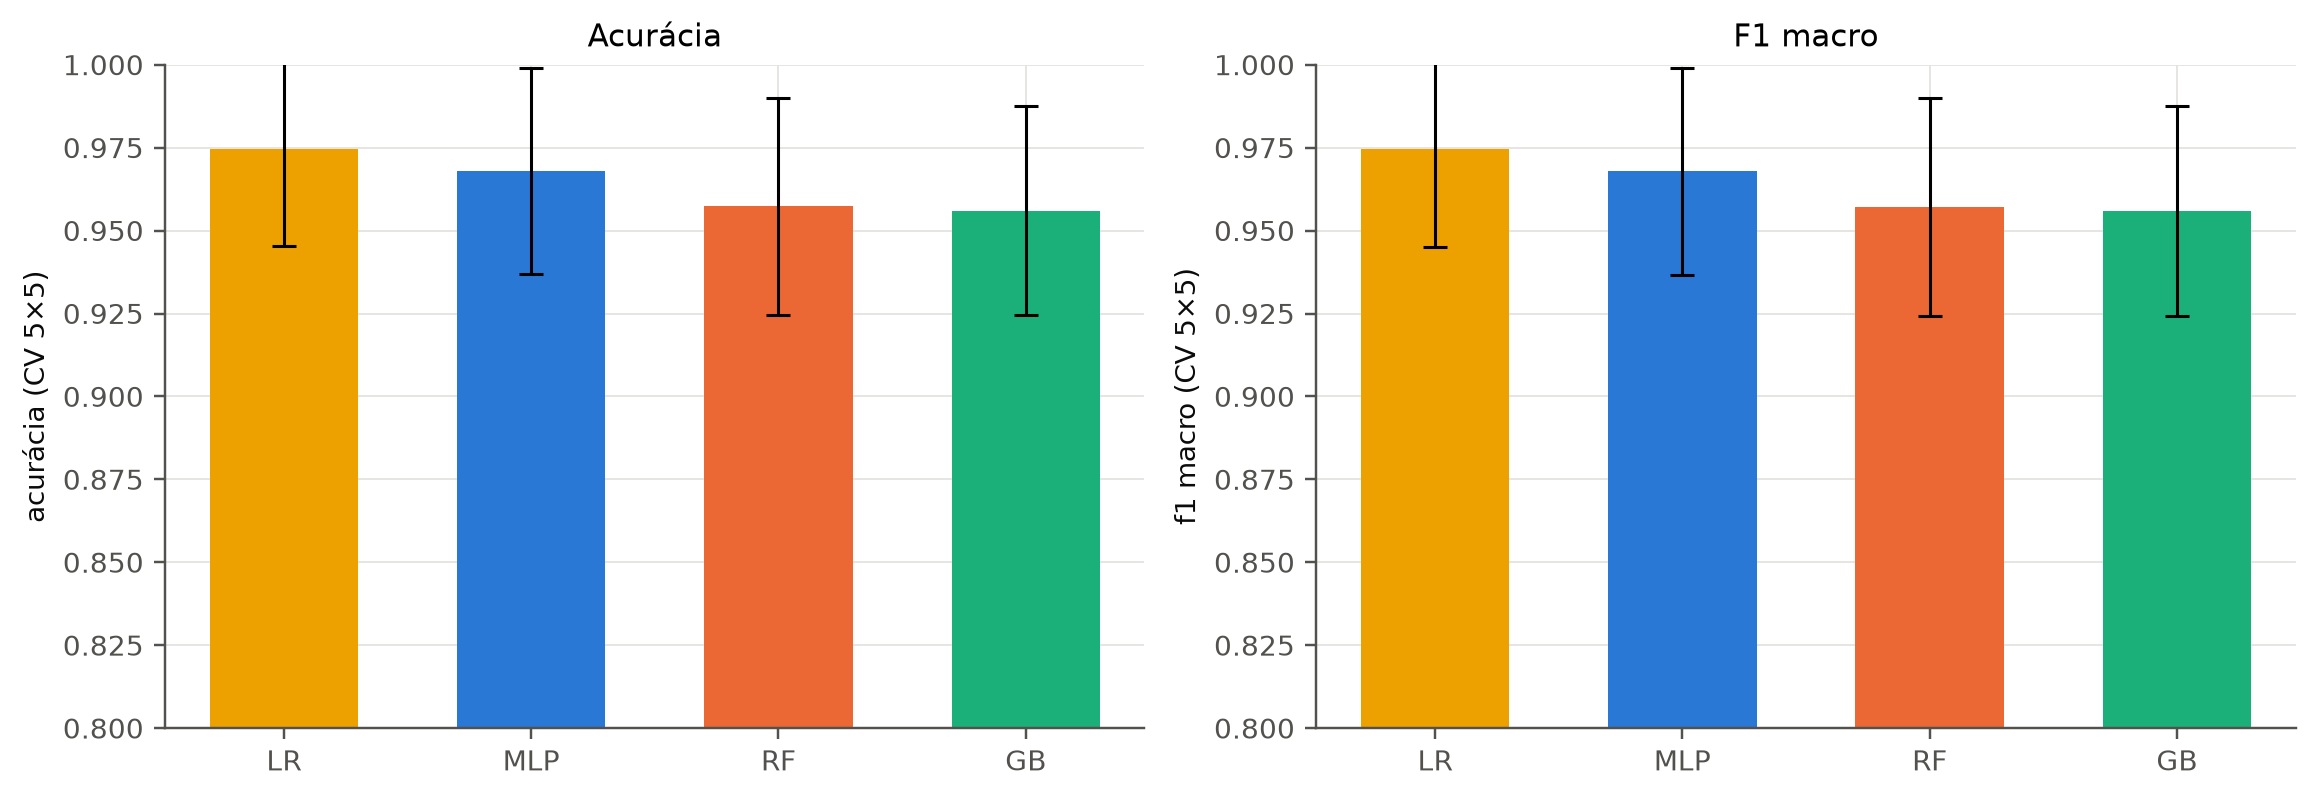
\includegraphics[width=\textwidth]{fig_comparacao_modelos.png}
	\caption{Acurácia e $F_1$ macro dos quatro modelos (validação cruzada 5 $\times$ 5). As barras
	de erro são $\pm 1$ desvio-padrão entre as 25 dobras.}
	\label{fig:comparacao}
\end{figure}

A ordenação é: regressão logística (\accLR{}), MLP (\accMLP{}), floresta aleatória (\accRF) e
\emph{gradient boosting} (\accGB). A regressão logística vence --- e vence com folga de tempo:
seus 25 ajustes levam uma fração de segundo, cerca de quarenta vezes menos que os da MLP
(\tabela{tab:modelos}).

A \tabela{tab:testes} traz o teste de Wilcoxon pareado para as três comparações.

\begin{table}[htbp]
	\centering
	\caption{Teste de Wilcoxon pareado entre a MLP e os demais modelos, sobre as 25 dobras de
	validação cruzada. A diferença é medida em pontos percentuais (MLP menos o outro modelo).}
	\label{tab:testes}
	% gerado automaticamente por mlp_iris.py - nao editar

\begin{tabular}{lrrr}
\toprule
\textbf{comparação} & \textbf{estatística W} & \textbf{valor p} & \textbf{diferença (p.p.)} \\
\midrule
MLP $\times$ RF & 3,5 & 0{,}033 & 1,07 \\
MLP $\times$ GB & 5,0 & 0{,}013 & 1,20 \\
MLP $\times$ LR & 0,0 & 0{,}025 & -0,67 \\
\bottomrule
\end{tabular}

\end{table}

As três diferenças são estatisticamente significativas ao nível de $5\,\%$: a MLP é melhor que a
floresta ($+1{,}07$ p.p., $p=\pRF$) e que o \emph{boosting} ($+1{,}20$ p.p., $p=\pGB$), e pior
que a regressão logística ($-0{,}67$ p.p., $p=\pLR$).

\paragraph{Como interpretar.} A significância estatística aqui mede consistência, não magnitude.
Uma diferença de $0{,}67$ ponto percentual é irrelevante na prática: corresponde a uma amostra em
150. O que os números realmente dizem é que, no Iris, os quatro modelos são essencialmente
equivalentes, e que qualquer afirmação de superioridade precisa de um conjunto maior para se
sustentar. A regressão logística leva vantagem por ser mais simples, mais rápida e igualmente
precisa --- exatamente o tipo de conclusão que o princípio da parcimônia recomenda.

\subsection{Efeito da padronização}

A \figura{fig:escala} compara o treinamento com e sem padronização, para Adam e para SGD com
momento.

\begin{figure}[htbp]
	\centering
	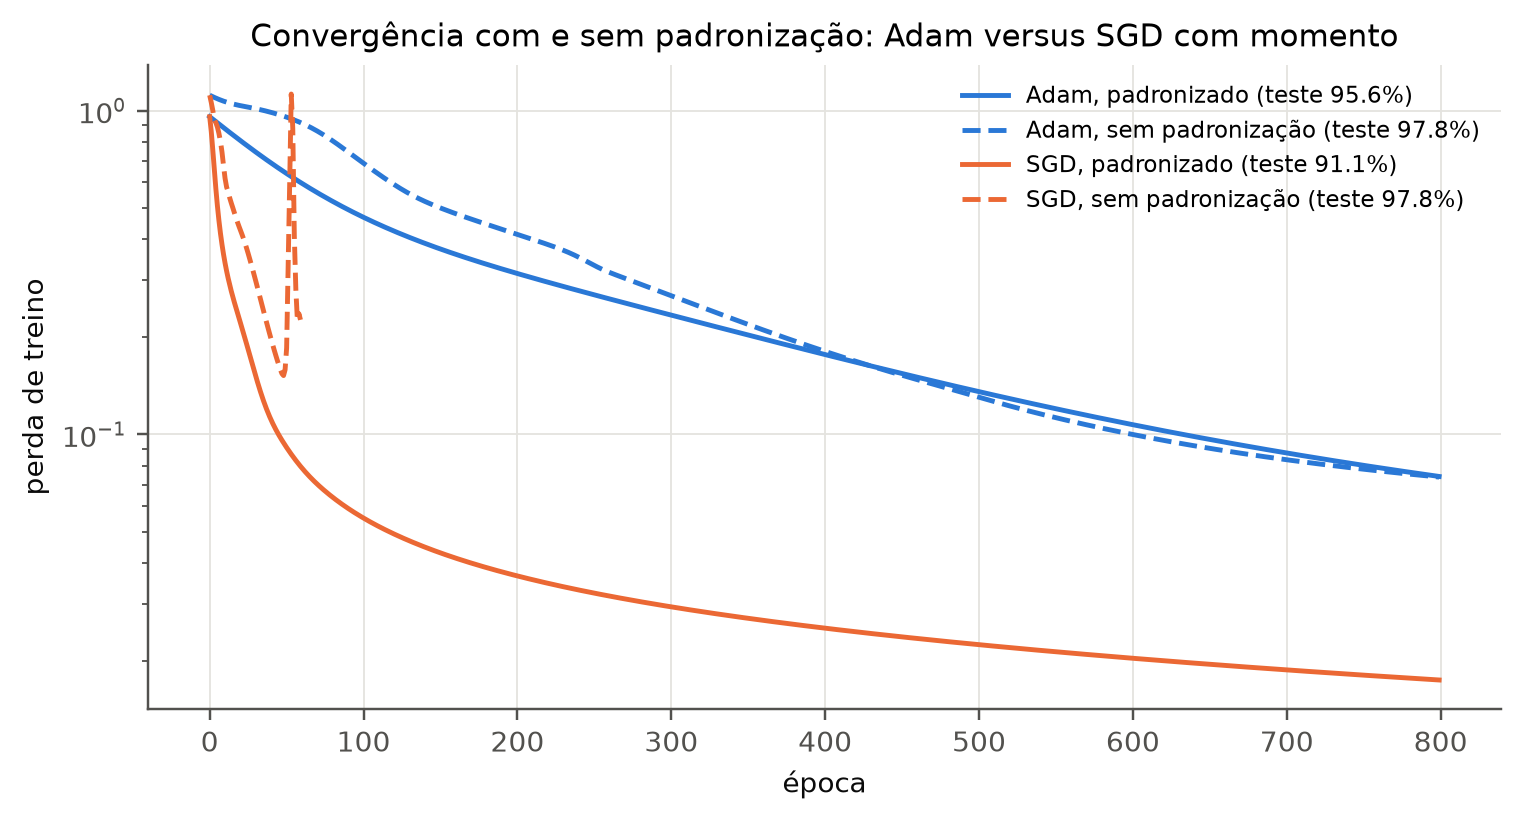
\includegraphics[width=0.82\textwidth]{fig_escala.png}
	\caption{Curvas de perda com e sem padronização dos atributos, para Adam (linhas contínuas) e
	SGD com momento (tracejadas). A acurácia indicada é a do conjunto de teste.}
	\label{fig:escala}
\end{figure}

Os resultados confirmam a teoria. Com Adam, as curvas com e sem padronização são quase idênticas:
o otimizador normaliza o passo por parâmetro e, por isso, é pouco sensível à escala. Com SGD, a
mesma taxa de aprendizado produz trajetórias muito diferentes: a versão sem padronização converge
em 60 épocas para uma perda de $0{,}23$, enquanto a versão padronizada precisa das 800 épocas para
chegar a $0{,}017$. A taxa adequada a uma escala não é adequada à outra.

A lição é prática: a padronização não é um ritual, é uma forma de tornar o problema independente
da escolha de taxa de aprendizado. Quando se usa um otimizador adaptativo como o Adam, ela é
quase cosmética; quando se usa SGD puro, ela é essencial. No Iris, como os atributos já estão em
centímetros e em faixas parecidas, o efeito sobre a acurácia final é pequeno --- mas o experimento
mostra por que o procedimento é adotado por padrão.

\subsection{Resumo dos resultados}

A \tabela{tab:resumo} consolida os números principais.

\begin{table}[htbp]
	\centering
	\caption{Síntese dos resultados do modelo principal.}
	\label{tab:resumo}
	\small
	\begin{tabular}{L{7.4cm} R{3.2cm}}
		\toprule
		\textbf{Item} & \textbf{Valor} \\
		\midrule
		Amostras (treino / teste) & \nTreino{} / \nTeste{} \\
		Atributos / classes & 4 / 3 \\
		Arquitetura & 4--16--3 \\
		Parâmetros treináveis & \parametrosMLP{} \\
		Acurácia (validação cruzada 5 $\times$ 5) & 96,8\,\% \\
		Acurácia (teste, $n=45$) & \accTeste{} \\
		Intervalo de confiança de Wilson (95\,\%) & [\icLo{}; \icHi{}] \\
		$F_1$ macro (teste) & \fmacroTeste{} \\
		Entropia cruzada (teste) & \llteste{} \\
		Épocas até a parada antecipada & \nIter{} \\
		Erro relativo máximo do gradiente & \erroGrad{} \\
		Acurácia da implementação em NumPy & \accNumpy{} \\
		\bottomrule
	\end{tabular}
\end{table}

% =======================================================================================================
\section{Discussão}
\label{sec:discussao}

Os resultados são simples de resumir e difíceis de interpretar. A rede acerta cerca de $97\,\%$
das amostras e erra três de quarenta e cinco no teste. Uma regressão logística acerta um pouco
mais, e ambos os resultados devem ser lidos com a mesma desconfiança saudável. Esta seção discute
o que os números significam, o que eles não significam e o que fazer com eles.

\subsection{Por que a rede não supera a regressão logística}

O resultado mais desconfortável --- e mais instrutivo --- é que a MLP não é superior a um modelo
linear. Há três evidências independentes apontando na mesma direção.

\paragraph{Evidência 1: a ativação identidade funciona tão bem quanto qualquer outra.}
Na \tabela{tab:ativacoes}, uma rede com ativação identidade na camada oculta --- que é
matematicamente equivalente a uma regressão logística multinomial --- obtém $96{,}0\,\%$ de
acurácia e a \emph{menor} entropia cruzada de todas as configurações ($0{,}083$). Se a não
linearidade estivesse capturando estrutura real, ela deveria produzir probabilidades melhores. Não
produz.

\paragraph{Evidência 2: as fronteiras de decisão são retas.}
A \figura{fig:fronteira-comparacao} mostra que a MLP e a regressão logística produzem fronteiras
praticamente idênticas no plano da pétala. A rede \emph{poderia} desenhar curvas; ela escolhe
retas, porque a regularização e os dados não justificam o contrário.

\paragraph{Evidência 3: a capacidade não ajuda.}
A \tabela{tab:arquiteturas} mostra que a acurácia é plana entre 35 e 9\,091 parâmetros. Se o
problema exigisse uma fronteira curva, redes maiores deveriam vencer. Elas não vencem --- e as
maiores perdem ligeiramente, por variância.

A explicação é geométrica: as três classes do Iris estão organizadas ao longo de uma direção
principal, com a \emph{setosa} separada e as outras duas quase separadas por um plano. Um modelo
linear já expressa essa estrutura; camadas ocultas adicionam graus de liberdade que o problema não
usa.

\subsection{Então para que serve a MLP aqui?}

Seria um erro concluir que a MLP é inútil. O que o experimento mostra é mais específico: \emph{neste
conjunto de dados}, a rede não tem vantagem. Ela continua sendo o modelo adequado quando:

\begin{itemize}
	\item a fronteira é comprovadamente não linear (dados de sensores, imagens, séries temporais
	      com regimes);
	\item há interações entre atributos que um modelo aditivo não captura;
	\item o volume de dados é suficiente para estimar os parâmetros extras --- o que não é o caso
	      de 150 amostras;
	\item há mais de uma dezena de atributos relevantes, situação em que a rede pode aprender
	      representações intermediárias.
\end{itemize}

O valor didático do Iris está justamente aí: ele mostra que \emph{mais modelo} não é sinônimo de
\emph{melhor modelo}. Escolher a complexidade certa é parte do problema, não um detalhe posterior.

\subsection{O papel da validação}

A diferença entre a estimativa de validação cruzada ($96{,}8\,\%$) e a de teste ($93{,}3\,\%$) é o
lembrete de que nenhuma estimativa é exata. Três fontes de incerteza atuam em conjunto:

\begin{enumerate}
	\item \textbf{amostragem}: 45 amostras de teste produzem um intervalo de confiança de quase 16
	      pontos percentuais;
	\item \textbf{partição}: a validação cruzada depende de como as dobras são formadas; o desvio
	      entre dobras foi de cerca de 3 pontos;
	\item \textbf{seleção}: a configuração foi escolhida olhando os resultados de validação
	      cruzada, o que introduz um viés otimista de magnitude desconhecida.
\end{enumerate}

A terceira fonte é a mais sutil. Quando se testam 9 arquiteturas, 4 ativações e 17 valores de
$\alpha$, o melhor resultado entre centenas de combinações é necessariamente favorecido pelo acaso.
A forma rigorosa de lidar com isso é a \emph{validação cruzada aninhada}: uma cruzada externa
estima o desempenho e uma interna seleciona hiperparâmetros, tudo dentro de cada dobra externa.
Neste relatório, o conjunto de teste reservado cumpre parcialmente esse papel, mas uma única
divisão ainda é uma amostra de tamanho 1 do processo de divisão.

\subsection{Limitações do estudo}

\begin{itemize}
	\item \textbf{uma única divisão treino/teste}. Repetir a divisão 30 vezes e reportar a
	      distribuição das acurácias daria uma estimativa mais estável que um único número;
	\item \textbf{sem análise de calibração}. Acurácia e entropia cruzada não mostram se as
	      probabilidades são confiáveis. Um diagrama de confiabilidade (\emph{reliability diagram})
	      e o escore de Brier completariam o diagnóstico;
	\item \textbf{importância por permutação com atributos correlacionados}. Comprimento e largura
	      da pétala têm correlação $0{,}96$; a importância de um é subestimada porque o outro
	      substitui a informação. Métodos como SHAP lidam melhor com esse caso;
	\item \textbf{apenas um conjunto de dados}. As conclusões sobre arquitetura e regularização
	      valem para o Iris. Não devem ser extrapoladas para outros domínios sem verificação;
	\item \textbf{sem busca exaustiva}. A varredura de hiperparâmetros foi em grade, não bayesiana,
	      e não incluiu \emph{dropout}, \emph{batch normalization} ou \emph{learning rate schedule}.
\end{itemize}

Nenhuma dessas limitações invalida os resultados; elas delimitam o alcance das afirmações. Um
relatório que não as declara está incompleto, não importa quão bom seja o número.

\subsection{O que o Iris não permite concluir}

Vale ser explícito sobre algumas conclusões que \emph{não} podem ser tiradas deste estudo:

\begin{itemize}
	\item que redes neurais são piores que modelos lineares em geral;
	\item que arquiteturas profundas não funcionam;
	\item que a regularização não importa;
	\item que o número de parâmetros deve ser sempre pequeno.
\end{itemize}

O que se pode afirmar é mais modesto e mais útil: em um problema com 150 amostras, quatro
atributos e classes quase linearmente separáveis, uma rede pequena é suficiente e um modelo
linear é competitivo. A complexidade do modelo deve acompanhar a complexidade do problema --- e a
única forma de saber é medir.

\subsection{Lições práticas}

O estudo sugere um roteiro para quem vai aplicar uma MLP a um problema tabular:

\begin{enumerate}
	\item \textbf{olhe os dados antes}. Um gráfico de dispersão e uma matriz de correlação evitam
	      semanas de ajuste inútil;
	\item \textbf{comece simples}. Uma regressão logística é um \emph{baseline} obrigatório; se a
	      rede não a supera, a rede não se justifica;
	\item \textbf{padronize dentro do pipeline}. O pré-processamento deve ser ajustado apenas no
	      treino de cada dobra;
	\item \textbf{reserve um teste}. E não o olhe até o final;
	\item \textbf{varie uma coisa por vez}. Arquitetura, ativação e regularização interagem, mas
	      varreduras simultâneas escondem qual fator causou o quê;
	\item \textbf{reporte incerteza}. Uma acurácia sem intervalo de confiança é uma meia-verdade;
	\item \textbf{verifique o gradiente}. Se você implementou a retropropagação, compare com
	      diferenças finitas antes de confiar no resultado;
	\item \textbf{compare com o custo}. A MLP levou 40 vezes mais tempo que a regressão logística
	      para um resultado ligeiramente pior. Em produção, isso importa.
\end{enumerate}

\subsection{Trabalhos futuros}

Três extensões naturais deste estudo são:

\begin{itemize}
	\item \textbf{validação cruzada aninhada} com correção para múltiplas comparações, para
	      quantificar o viés de seleção;
	\item \textbf{calibração}: curvas de confiabilidade, escore de Brier e \emph{temperature
	      scaling}, que mostram se a rede sabe \emph{o quanto} está incerta;
	\item \textbf{extensão para outros conjuntos}: repetir o protocolo em bases com fronteiras
	      comprovadamente não lineares (por exemplo, \emph{two moons}, \emph{circles} e dados de
	      sensores) para contrastar com o que foi observado no Iris.
\end{itemize}

% =======================================================================================================
\section{Conclusão}
\label{sec:conclusao}

Este relatório construiu, treinou, avaliou e interpretou uma rede perceptron multicamadas para o
conjunto de dados Iris. O percurso foi deliberadamente completo: da formulação do neurônio
artificial à derivação da retropropagação, do protocolo de validação à comparação estatística com
modelos alternativos.

\paragraph{O que foi feito.} Uma rede com uma camada oculta de 16 neurônios, ativação tangente
hiperbólica e regularização $L_2$ foi ajustada com o otimizador Adam sobre \nTreino{} amostras
padronizadas. A seleção de arquitetura, ativação e regularização foi feita por validação cruzada
estratificada repetida, com o pré-processamento dentro do \texttt{Pipeline} para evitar vazamento.
O desempenho final foi medido uma única vez em \nTeste{} amostras reservadas.

\paragraph{O que foi obtido.} A acurácia média em validação cruzada foi de \accMLP{}, com desvio de
\sdMLP{} entre dobras. No conjunto de teste, a rede acertou \accTeste{} das amostras (intervalo de
confiança de $95\,\%$: \icLo{} a \icHi{}), com $F_1$ macro de \fmacroTeste{} e entropia cruzada de
\llteste{}. Os erros se concentram na fronteira entre \emph{versicolor} e \emph{virginica}, e a
\emph{setosa} foi classificada sem erro.

\paragraph{O que foi verificado.} A implementação da retropropagação foi validada por diferenças
centrais, com erro relativo máximo de \erroGrad{} --- muito abaixo do limiar de $10^{-4}$. Uma
implementação independente em NumPy, com o gradiente escrito à mão, reproduziu a mesma acurácia da
biblioteca (\accNumpy{}). A concordância entre duas implementações independentes é a evidência
mais forte de que o resultado não é artefato de código.

\paragraph{O que foi aprendido.} Três conclusões se destacam, e nenhuma delas é sobre ``acertar
mais''.

\begin{enumerate}
	\item \textbf{a complexidade deve acompanhar o problema}. No Iris, uma rede de 35 parâmetros
	      iguala ou supera redes de 9\,091 parâmetros. O excesso de capacidade não trouxe ganho,
	      trouxe variância;
	\item \textbf{o modelo mais simples é um adversário honesto}. A regressão logística
	      (\accLR{}) superou a rede por uma margem pequena mas consistente
	      ($p=\pLR$). Em um problema quase linearmente separável, um modelo linear é a linha de
	      base que qualquer método mais complexo precisa justificar;
	\item \textbf{a incerteza é parte do resultado}. A diferença de $3{,}5$ pontos entre validação
	      cruzada e teste, e o intervalo de confiança de 16 pontos percentuais, mostram que
	      reportar um único número seria enganoso. A avaliação honesta inclui a variabilidade.
\end{enumerate}

\paragraph{Contribuições.} O trabalho deixa um artefato reproduzível: o script
\texttt{mlp\_iris.py}, que executa a análise de ponta a ponta e gera todas as figuras, tabelas e
números citados neste documento. Deixa também uma exposição didática da matemática da MLP, com
derivação completa no apêndice, e um protocolo de avaliação que pode ser transplantado para outros
conjuntos tabulares.

\paragraph{Consideração final.} O Iris é frequentemente apresentado como um problema resolvido, e
é --- mas o que ele ensina não é que as redes neurais funcionam. Ensina que a escolha do modelo é
uma decisão informada por evidência, que a avaliação correta é mais difícil que o treinamento e
que um resultado negativo, bem medido, vale mais que um resultado positivo mal medido. Uma rede
que acerta $97\,\%$ e sabe explicar por que não acerta $100\,\%$ é mais útil que uma que reporta
$99{,}9\,\%$ sem saber de onde veio o número.

% =======================================================================================================
\appendix
\section{Derivação completa da retropropagação}
\label{ap:backprop}

Esta seção apresenta a derivação passo a passo, com as dimensões de cada objeto. A notação segue o
\secao{sec:mlp}.

\subsection{Notação e dimensões}

\begin{itemize}
	\item $m$: número de amostras no minilote; $d$: número de atributos; $C$: número de classes;
	\item $n_l$: número de neurônios da camada $l$, com $n_0 = d$ e $n_L = C$;
	\item $\bX \in \R^{m\times d}$, com uma amostra por linha;
	\item $\bW^{(l)} \in \R^{n_{l-1}\times n_l}$, $\bb^{(l)} \in \R^{n_l}$;
	\item $\bZ^{(l)} \in \R^{m\times n_l}$ e $\bA^{(l)} = f_l(\bZ^{(l)}) \in \R^{m\times n_l}$;
	\item $\bY \in \{0,1\}^{m\times C}$ (rótulos em \emph{one-hot}) e $\bP \in (0,1)^{m\times C}$
	      (probabilidades previstas).
\end{itemize}

A perda é a média das entropias cruzadas mais a penalidade $L_2$:
\begin{equation}
	\Loss = \frac{1}{m}\sum_{i=1}^{m}\ell_i + \frac{\lambda}{2}\sum_{l=1}^{L}\left\|\bW^{(l)}\right\|_F^2,
	\qquad
	\ell_i = -\sum_{k=1}^{C} y_{ik}\log p_{ik}.
	\label{eq:ap-perda}
\end{equation}

\subsection{Gradiente da entropia cruzada em relação aos logits}

A softmax da amostra $i$ é
\begin{equation}
	p_{ik} = \frac{e^{z_{ik}}}{S_i},
	\qquad S_i = \sum_{j=1}^{C} e^{z_{ij}}.
\end{equation}

Derivando em relação a um logit $z_{i\ell}$, com a regra do quociente:
\begin{align}
	\frac{\partial p_{ik}}{\partial z_{i\ell}}
	&= \frac{\delta_{k\ell}\,e^{z_{ik}}S_i - e^{z_{ik}}e^{z_{i\ell}}}{S_i^2} \nonumber\\
	&= \frac{e^{z_{ik}}}{S_i}\delta_{k\ell} - \frac{e^{z_{ik}}}{S_i}\frac{e^{z_{i\ell}}}{S_i}
	= p_{ik}\left(\delta_{k\ell} - p_{i\ell}\right),
	\label{eq:ap-jacobiano}
\end{align}
com $\delta_{k\ell}=1$ se $k=\ell$ e $0$ caso contrário. Agora derive a perda da amostra:
\begin{align}
	\frac{\partial \ell_i}{\partial z_{i\ell}}
	&= -\sum_{k=1}^{C} y_{ik}\frac{1}{p_{ik}}\frac{\partial p_{ik}}{\partial z_{i\ell}}
	= -\sum_{k=1}^{C} y_{ik}\left(\delta_{k\ell} - p_{i\ell}\right) \nonumber\\
	&= -\sum_{k=1}^{C} y_{ik}\delta_{k\ell} + p_{i\ell}\sum_{k=1}^{C} y_{ik}
	= -y_{i\ell} + p_{i\ell},
	\label{eq:ap-pmenosy}
\end{align}
onde se usou $\sum_k y_{ik}=1$, válido porque os rótulos são \emph{one-hot}. Logo,
\begin{equation}
	\frac{\partial \Loss}{\partial \bZ^{(L)}} = \frac{1}{m}\left(\bP - \bY\right) \;\equiv\; \bm{\Delta}^{(L)}.
	\label{eq:ap-deltaL}
\end{equation}

O fator $1/m$ vem de a perda ser uma média. Ele é frequentemente esquecido em implementações
manuais, e o sintoma é uma taxa de aprendizado que ``precisa'' ser $m$ vezes maior.

\subsection{Retropropagando o erro}

Suponha conhecido $\bm{\Delta}^{(l)} = \partial\Loss/\partial\bZ^{(l)}$. Para obter o erro da
camada anterior, aplica-se a regra da cadeia em duas etapas.

\paragraph{Passo 1: da pré-ativação para a ativação da camada anterior.} Como
$\bZ^{(l)} = \bA^{(l-1)}\bW^{(l)} + \mathbf{1}\bb^{(l)\top}$,
\begin{equation}
	\frac{\partial \Loss}{\partial \bA^{(l-1)}} = \bm{\Delta}^{(l)}\,\bW^{(l)\top}
	\;\in\; \R^{m\times n_{l-1}}.
	\label{eq:ap-dA}
\end{equation}

\paragraph{Passo 2: da ativação para a pré-ativação.} Como a ativação é aplicada elemento a
elemento, $\bA^{(l-1)} = f_{l-1}(\bZ^{(l-1)})$ e
\begin{equation}
	\bm{\Delta}^{(l-1)} = \frac{\partial \Loss}{\partial \bA^{(l-1)}} \odot f_{l-1}'\!\left(\bZ^{(l-1)}\right),
	\label{eq:ap-rec}
\end{equation}
com $\odot$ o produto de Hadamard. Substituindo \equacao{eq:ap-dA} em \equacao{eq:ap-rec}:
\begin{equation}
	\boxed{\;\bm{\Delta}^{(l-1)} = \left(\bm{\Delta}^{(l)}\bW^{(l)\top}\right)\odot f_{l-1}'\!\left(\bZ^{(l-1)}\right)\;}
	\label{eq:ap-rec-final}
\end{equation}

\subsection{Gradientes dos parâmetros}

Para os pesos, $\partial z_{ij}^{(l)}/\partial W_{ab}^{(l)} = A_{ia}^{(l-1)}$ se $b=j$ e $0$ caso
contrário. Aplicando a regra da cadeia:
\begin{equation}
	\frac{\partial \Loss}{\partial W_{ab}^{(l)}}
	= \sum_{i=1}^{m}\frac{\partial \Loss}{\partial z_{ib}^{(l)}}\frac{\partial z_{ib}^{(l)}}{\partial W_{ab}^{(l)}}
	= \sum_{i=1}^{m}\Delta_{ib}^{(l)}A_{ia}^{(l-1)},
\end{equation}
que em forma matricial é
\begin{equation}
	\frac{\partial \Loss}{\partial \bW^{(l)}} = \bA^{(l-1)\top}\bm{\Delta}^{(l)} \;\in\; \R^{n_{l-1}\times n_l}.
	\label{eq:ap-gradW}
\end{equation}

Para os vieses, $\partial z_{ij}^{(l)}/\partial b_j^{(l)} = 1$ para toda amostra, logo
\begin{equation}
	\frac{\partial \Loss}{\partial \bb^{(l)}} = \sum_{i=1}^{m}\bm{\Delta}^{(l)}_{i,:}
	= \mathbf{1}_m^{\top}\bm{\Delta}^{(l)} \;\in\; \R^{n_l}.
	\label{eq:ap-gradb}
\end{equation}

\subsection{Efeito da regularização}

Derivando o termo $\frac{\lambda}{2}\|\bW^{(l)}\|_F^2 = \frac{\lambda}{2}\sum_{a,b}(W_{ab}^{(l)})^2$:
\begin{equation}
	\frac{\partial}{\partial \bW^{(l)}}\left[\frac{\lambda}{2}\left\|\bW^{(l)}\right\|_F^2\right]
	= \lambda\,\bW^{(l)}.
\end{equation}
Somando a \equacao{eq:ap-gradW}:
\begin{equation}
	\frac{\partial \Loss}{\partial \bW^{(l)}} = \bA^{(l-1)\top}\bm{\Delta}^{(l)} + \lambda\bW^{(l)}.
	\label{eq:ap-gradW-reg}
\end{equation}

\subsection{Algoritmo e complexidade}

O cálculo completo é:

\begin{enumerate}
	\item \textbf{propagação direta}: para $l=1,\dots,L$, calcule e armazene $\bZ^{(l)}$ e
	      $\bA^{(l)}$; calcule $\bP$;
	\item \textbf{erro de saída}: $\bm{\Delta}^{(L)} = (\bP-\bY)/m$;
	\item \textbf{para $l=L,\dots,1$}: calcule $\partial\Loss/\partial\bW^{(l)}$ e
	      $\partial\Loss/\partial\bb^{(l)}$; se $l>1$, calcule $\bm{\Delta}^{(l-1)}$;
	\item \textbf{atualize} os parâmetros com o otimizador escolhido.
\end{enumerate}

Cada passo custa $O(m\,n_{l-1}n_l)$ para a camada $l$; o total é
$O\!\left(m\sum_l n_{l-1}n_l\right)$, proporcional ao número de parâmetros multiplicado pelo
tamanho do minilote. A memória necessária é a das ativações armazenadas,
$O\!\left(m\sum_l n_l\right)$.

\subsection{Estabilidade numérica}

Calcular $p_{ik}$ diretamente pode estourar quando os logits são grandes, porque $e^{z}$ cresce
muito rápido. A implementação usa o truque do \emph{log-sum-exp}: subtrai-se o maior logit antes de
exponenciar,
\begin{equation}
	p_{ik} = \frac{\exp\!\left(z_{ik} - \max_j z_{ij}\right)}{\sum_j \exp\!\left(z_{ij} - \max_j z_{ij}\right)},
\end{equation}
o que não altera o resultado matemático (numerador e denominador são multiplicados pelo mesmo
fator) mas evita \emph{overflow}. No cálculo da perda, usa-se
$\log p_{ik} = z_{ik} - \log\sum_j e^{z_{ij}}$, que é estável mesmo quando $p_{ik}$ é muito
pequeno.

\subsection{Caso de uma amostra}

Para uso em SGD puro, $m=1$ e todos os somatórios sobre amostras desaparecem:
\begin{equation}
	\bm{\delta}^{(L)} = \bp - \by, \qquad
	\bm{\delta}^{(l-1)} = \left(\bm{\delta}^{(l)}\bW^{(l)\top}\right)\odot f'\!\left(\bz^{(l-1)}\right),
\end{equation}
\begin{equation}
	\frac{\partial \ell}{\partial \bW^{(l)}} = \ba^{(l-1)}\bm{\delta}^{(l)\top} + \lambda\bW^{(l)},
	\qquad
	\frac{\partial \ell}{\partial \bb^{(l)}} = \bm{\delta}^{(l)}.
\end{equation}
É comum, na prática, usar a forma com $m=1$ e uma taxa de aprendizado menor, já que o gradiente
de uma amostra é uma estimativa ruidosa do gradiente verdadeiro.

% =======================================================================================================
\section{Tabelas auxiliares}
\label{ap:tabelas}

\begin{table}[htbp]
	\centering
	\caption{Pesos da camada de entrada de uma rede $4$--$8$--$3$ treinada em todos os dados
	(valores arredondados).}
	\label{tab:pesos}
	\small
	% gerado automaticamente por mlp_iris.py - nao editar

\begin{tabular}{lrrrrrrrr}
\toprule
\textbf{atributo} & \textbf{h1} & \textbf{h2} & \textbf{h3} & \textbf{h4} & \textbf{h5} & \textbf{h6} & \textbf{h7} & \textbf{h8} \\
\midrule
SL & -0{,}13 & 0{,}73 & 0{,}78 & 0{,}37 & -1{,}03 & -0{,}81 & -0{,}33 & 0{,}67 \\
SW & 0{,}09 & -0{,}12 & -1{,}16 & 0{,}42 & 1{,}01 & -0{,}04 & -0{,}73 & -0{,}49 \\
PL & -0{,}23 & 0{,}54 & 0{,}50 & -0{,}04 & -0{,}36 & -0{,}90 & 0{,}09 & -0{,}71 \\
PW & -0{,}02 & 1{,}03 & 0{,}20 & 0{,}27 & -0{,}36 & -1{,}02 & 0{,}54 & -0{,}97 \\
\bottomrule
\end{tabular}

\end{table}

\begin{table}[htbp]
	\centering
	\caption{Hiperparâmetros do modelo principal e dos modelos de referência.}
	\label{tab:hiper}
	\small
	\begin{tabular}{L{3.4cm} L{10.2cm}}
		\toprule
		\textbf{Modelo} & \textbf{Configuração} \\
		\midrule
		MLP &
		padronização $+$ 16 neurônios, ativação \emph{tanh}, $\alpha=10^{-2}$, Adam,
		$\eta_0=10^{-3}$, máximo de 3000 épocas \\
		RF &
		padronização $+$ 400 árvores, folha mínima de 1 amostra, semente 42 \\
		GB &
		padronização $+$ 300 estimadores, taxa $0{,}06$, profundidade 3, subamostra $0{,}9$ \\
		LR &
		padronização $+$ regressão logística multinomial, $C=10$, máximo de 2000 iterações \\
		\bottomrule
	\end{tabular}
\end{table}

% =======================================================================================================
\section{Como reproduzir}
\label{ap:repro}

\subsection{Requisitos}

O código foi executado com Python 3.15 e as bibliotecas listadas em \texttt{requirements.txt} do
projeto: NumPy 2.5, pandas 3.1, scikit-learn 1.9, SciPy 1.18, Matplotlib 3.11 e joblib 1.6. Não há
dependência de GPU nem de bibliotecas de aprendizado profundo: toda a rede é implementada em
NumPy/scikit-learn.

\subsection{Execução}

A partir da pasta \texttt{MLP/}:

\begin{lstlisting}[language=bash,caption={Comandos para reproduzir a análise e compilar o relatório.},label={lst:repro}]
.venv/Scripts/python.exe iris/mlp_iris.py
cd iris/artigo
pdflatex relatorio.tex
pdflatex relatorio.tex
\end{lstlisting}

O script grava as figuras em \texttt{artigo/figuras/}, as tabelas em \texttt{artigo/tabelas/}, os
números em \texttt{artigo/numeros.tex} e as métricas em CSV na pasta \texttt{resultados/}. A
execução completa leva cerca de quatro minutos.

\subsection{Estrutura dos arquivos}

\begin{lstlisting}[caption={Organização da pasta \texttt{iris/}.},label={lst:estrutura}]
iris/
  mlp_iris.py            codigo completo da analise
  resultados/            metricas em CSV, resumo em Markdown, log
  artigo/
    relatorio.tex        documento principal
    numeros.tex          macros geradas pela execucao
    secoes/              texto por secao
    figuras/             figuras em PNG (220 dpi)
    tabelas/             tabelas em LaTeX (booktabs)
\end{lstlisting}

\subsection{Como citar os números}

O arquivo \texttt{numeros.tex} define macros como \verb|\accMLP| e \verb|\erroGrad|, usadas ao
longo do texto. Se o script for reexecutado com outra semente, os valores mudam e o documento é
recompilado automaticamente com os novos números --- não há transcrição manual para desatualizar.


% =======================================================================================================
\begin{thebibliography}{99}
\addcontentsline{toc}{section}{Referências}

\bibitem{fisher1936}
FISHER, R. A. The use of multiple measurements in taxonomic problems.
\emph{Annals of Eugenics}, v.~7, n.~2, p.~179--188, 1936.

\bibitem{anderson1935}
ANDERSON, E. The irises of the Gaspé Peninsula.
\emph{Bulletin of the American Iris Society}, v.~59, p.~2--5, 1935.

\bibitem{mcculloch1943}
McCULLOCH, W. S.; PITTS, W. A logical calculus of the ideas immanent in nervous activity.
\emph{Bulletin of Mathematical Biophysics}, v.~5, p.~115--133, 1943.

\bibitem{rosenblatt1958}
ROSENBLATT, F. The perceptron: a probabilistic model for information storage and organization
in the brain. \emph{Psychological Review}, v.~65, n.~6, p.~386--408, 1958.

\bibitem{minsky1969}
MINSKY, M.; PAPERT, S. \emph{Perceptrons: an introduction to computational geometry}.
Cambridge: MIT Press, 1969.

\bibitem{rumelhart1986}
RUMELHART, D. E.; HINTON, G. E.; WILLIAMS, R. J. Learning representations by back-propagating
errors. \emph{Nature}, v.~323, p.~533--536, 1986.

\bibitem{cybenko1989}
CYBENKO, G. Approximation by superpositions of a sigmoidal function.
\emph{Mathematics of Control, Signals and Systems}, v.~2, p.~303--314, 1989.

\bibitem{hornik1989}
HORNIK, K.; STINCHCOMBE, M.; WHITE, H. Multilayer feedforward networks are universal
approximators. \emph{Neural Networks}, v.~2, n.~5, p.~359--366, 1989.

\bibitem{lecun1998}
LECUN, Y.; BOTTOU, L.; ORR, G. B.; MÜLLER, K.-R. Efficient backprop.
In: \emph{Neural Networks: Tricks of the Trade}. Berlin: Springer, 1998. p.~9--50.

\bibitem{glorot2010}
GLOROT, X.; BENGIO, Y. Understanding the difficulty of training deep feedforward neural
networks. In: \emph{Proceedings of AISTATS}, 2010. p.~249--256.

\bibitem{he2015}
HE, K.; ZHANG, X.; REN, S.; SUN, J. Delving deep into rectifiers: surpassing human-level
performance on ImageNet classification. In: \emph{Proceedings of ICCV}, 2015. p.~1026--1034.

\bibitem{srivastava2014}
SRIVASTAVA, N.; HINTON, G.; KRIZHEVSKY, A.; SUTSKEVER, I.; SALAKHUTDINOV, R. Dropout: a simple
way to prevent neural networks from overfitting. \emph{Journal of Machine Learning Research},
v.~15, p.~1929--1958, 2014.

\bibitem{kingma2015}
KINGMA, D. P.; BA, J. Adam: a method for stochastic optimization.
In: \emph{Proceedings of ICLR}, 2015.

\bibitem{prechelt1998}
PRECHELT, L. Early stopping --- but when?
In: \emph{Neural Networks: Tricks of the Trade}. Berlin: Springer, 1998. p.~55--69.

\bibitem{breiman2001}
BREIMAN, L. Random forests. \emph{Machine Learning}, v.~45, p.~5--32, 2001.

\bibitem{friedman2001}
FRIEDMAN, J. H. Greedy function approximation: a gradient boosting machine.
\emph{Annals of Statistics}, v.~29, n.~5, p.~1189--1232, 2001.

\bibitem{pedregosa2011}
PEDREGOSA, F. et al. Scikit-learn: machine learning in Python.
\emph{Journal of Machine Learning Research}, v.~12, p.~2825--2830, 2011.

\bibitem{bishop2006}
BISHOP, C. M. \emph{Pattern recognition and machine learning}. New York: Springer, 2006.

\bibitem{goodfellow2016}
GOODFELLOW, I.; BENGIO, Y.; COURVILLE, A. \emph{Deep learning}. Cambridge: MIT Press, 2016.

\bibitem{haykin2009}
HAYKIN, S. \emph{Neural networks and learning machines}. 3.~ed. New York: Pearson, 2009.

\bibitem{kaufman2012}
KAUFMAN, S.; ROSSET, S.; PERLICH, C.; STITES, B. Leakage in data mining: formulation, detection,
and avoidance. \emph{ACM Transactions on Knowledge Discovery from Data}, v.~6, n.~4, p.~1--21, 2012.

\bibitem{roberts2017}
ROBERTS, D. R. et al. Cross-validation strategies for data with temporal, spatial, hierarchical,
or phylogenetic structure. \emph{Ecography}, v.~40, n.~8, p.~913--929, 2017.

\bibitem{dietterich1998}
DIETTERICH, T. G. Approximate statistical tests for comparing supervised classification learning
algorithms. \emph{Neural Computation}, v.~10, n.~7, p.~1895--1923, 1998.

\bibitem{demsar2006}
DEMŠAR, J. Statistical comparisons of classifiers over multiple data sets.
\emph{Journal of Machine Learning Research}, v.~7, p.~1--30, 2006.

\bibitem{kohavi1995}
KOHAVI, R. A study of cross-validation and bootstrap for accuracy estimation and model selection.
In: \emph{Proceedings of IJCAI}, 1995. p.~1137--1143.

\bibitem{sklearn-iris}
SCIKIT-LEARN. \emph{The Iris dataset}. Exemplo da documentação oficial.
Disponível em: \url{https://scikit-learn.org/1.4/auto_examples/datasets/plot_iris_dataset.html}.
Acesso em: 2026.

\bibitem{sklearn-mlp}
SCIKIT-LEARN. \emph{sklearn.neural\_network.MLPClassifier}.
Disponível em: \url{https://scikit-learn.org/stable/modules/generated/sklearn.neural_network.MLPClassifier.html}.
Acesso em: 2026.

\end{thebibliography}

\end{document}
